\begin{comment}
dead time: 185,212

eep: 55, 62, 256
Cherenkov radiation: 2, 51
muon (crossing EL region) : 107, 291,75, 
muon (anodic): 207
muon (cathodic): 7, 40 , 49
radiation
S1: 64, 210
anode cone: 47, (76,77), (175-177)
cathodic corner(or really close to cathode) :145, 67
EL region: 218,83
cathodic : 21,44
noise: 34
dark current: 53
PTFE fluo: 161(160),
ring radiation: 248, 181, 85, 105, 
grid radiation: 117
\end{comment}

\section{Signals}
\label{sec:events}
%An event  is the process that a particle interacts with the medium which then emit photons in the ELD. An event sometimes can be separated into sub-events, due to the time The study on the PMT photons pulses that we record from an event or a sub-event is the fundamental elements of the understanding of the detector performance, and leads to the understanding of the electron emission process. 
%Signals, PMT photon pulses that we record, are the fundamental elements of to understand detector activities. 
A variety of processes can give rise to signals in the detector. Based on their source origin, signals are separated to four different categories:
\begin{itemize}
	\item electron emission (both from the grid wires and from the grid rings)
	\item particle radiation from radioactive materials (both from inside and from outside the ELD),
	\item cosmic ray,
	\item and other miscellaneous sources, which include: 
	\begin{itemize}
		\item electronic noise %(from the electrical ground of the building and other powered devices, e.g. the KNF circulation pump.)
		\item PMT dark current, 
		\todo{\item PMT afterpulsing,}
		\item PTFE cone reflector fluorescence, 
		\item Cherenkov radiation (in PTFE cone reflectors and PMT windows)%(created in the PTFE cone reflectors and the PMT windows when a charge particle, most likely an electron or a muon, passes through),
		\item discharge, as in a short-lived plasma in the medium, i.e., breakdown.
	\end{itemize}
\end{itemize}

\subsection{Electron emission} 
\label{sec:events ee}
Electron emission signals, especially those from the grid wires, are our signals of interest. A cartoon of the physical process and an example waveform of \ees s are shown in Fig.~\ref{fig:ElectronEmissionPulse}. An electron leaves the cathodic electrode from various types of emission processes. After the electron left the wire surface, the high electric field around the cathodic wire will quickly energize the electron. The high energy electron then ionizes and excites the atoms around it. The process in which more drifted electrons are produced is called electron multiplication; since in this particular case, the electron multiplication process happens near the cathodic electrode, it is also called the cathodic gas gain. In the high electric field region around the cathodic wire, more EL light is produced per unit of time compared to a lower electric field region. This is the cause of the ``peak" at the beginning of the \ees .  Next, these electrons drift to the anodic electrode according to the voltage difference between the two grids, producing EL light along the drift. This process is responsible for the majority of EL light seen in the \ees . There is a clear start and stop time for the \ees . The time difference between the two times (\ees\ duration) is approximate to the duration of this drift. Then, drifted electrons get close to the high electric field region around the anodic electrode. Because of  the high electric field, drifted electrons also go through a similar electron multiplication process in this high electric field region, which is also called the anodic gas gain. This process also creates more electrons and a higher production rate of EL light, resulting in a ``peak" at the ending of the \ees . The peak at the end of the signal is lower than the peak at the beginning of the signal. This is resulting from the dispersion of the arrival times of drifted electrons on anodic electrode, because the different microscopic trajectory each drifted electron takes to reach the anodic electrode. The different arrival times of the drifted electrons cause the final increment of EL light production from different electrons do not happen coincidently. This lowers the height of the peak at the ending of the \ees . Another reason for the difference in height of the peaks is because the electric field on the anodic wire is smaller than that of cathodic wire with regard to the wire diameter of the anodic wire are larger, which therefore results in a smaller production of EL light.

\begin{figure}[!htbp]
	\centering
	\begin{subfigure}[b]{\figurewidth}
		\centering
		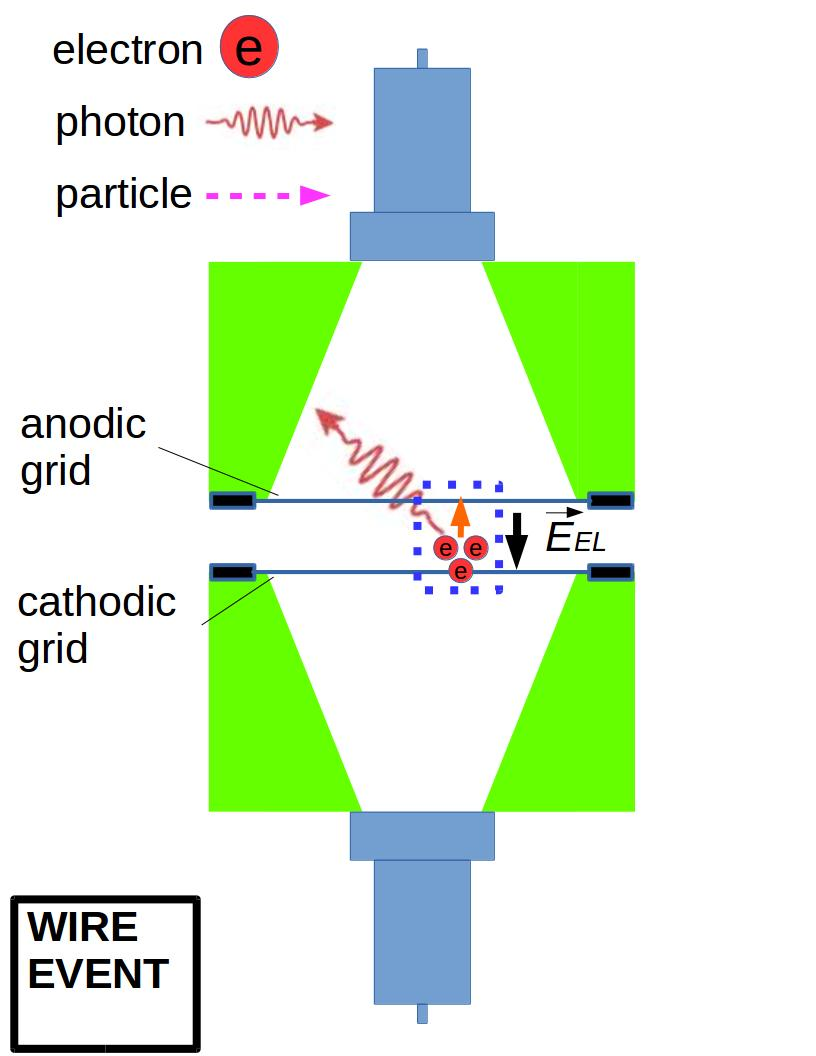
\includegraphics[width=\halfwidth,clip,trim={0 0 0 0},angle=0,origin=c]{Figures/GasTest/WeiDrawEvent/WirePhotoF.jpg}
%		\caption{}
%		\label{fig:ElectronEmissionPulse a}
%	\end{subfigure}
%	\begin{subfigure}[b]{\halfwidth}
%		\centering
	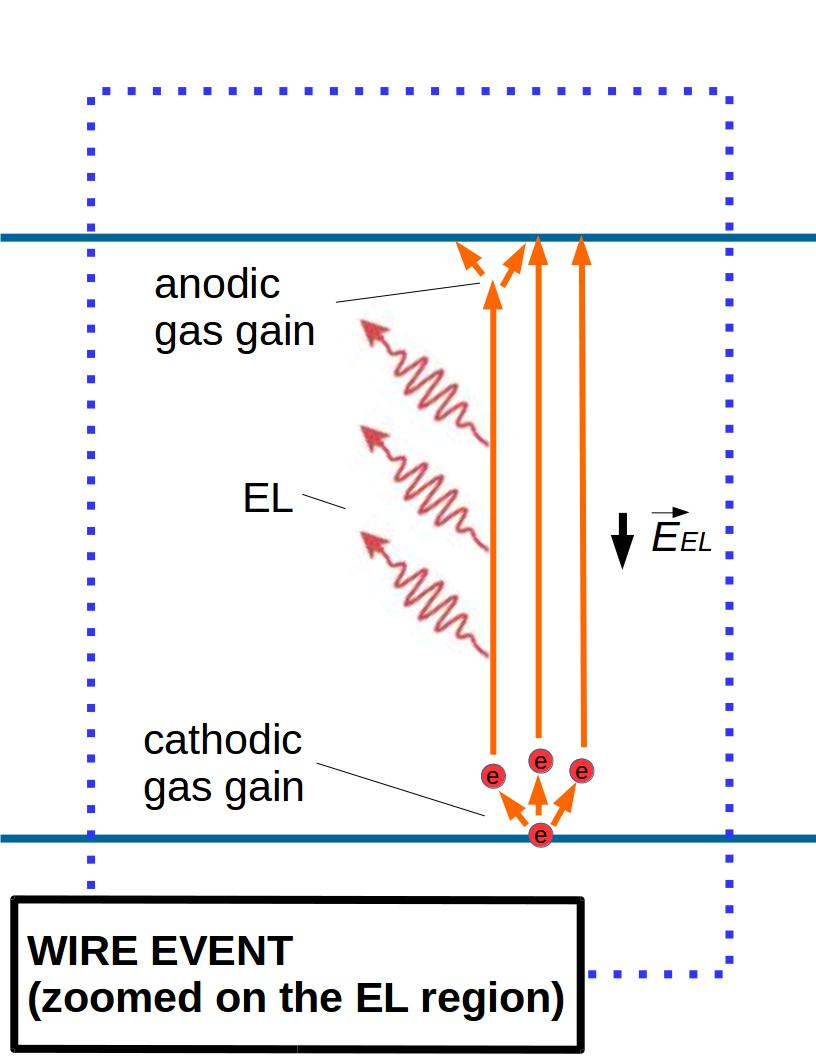
\includegraphics[width=\halfwidth,clip,trim={0 0 0 0}]{Figures/GasTest/WeiDrawEvent/WirePhotoZ.jpg}
		\caption{}
		\label{fig:ElectronEmissionPulse b}
	\end{subfigure}
    \par\bigskip
	\begin{subfigure}[b]{0.8\textwidth}
	\centering
	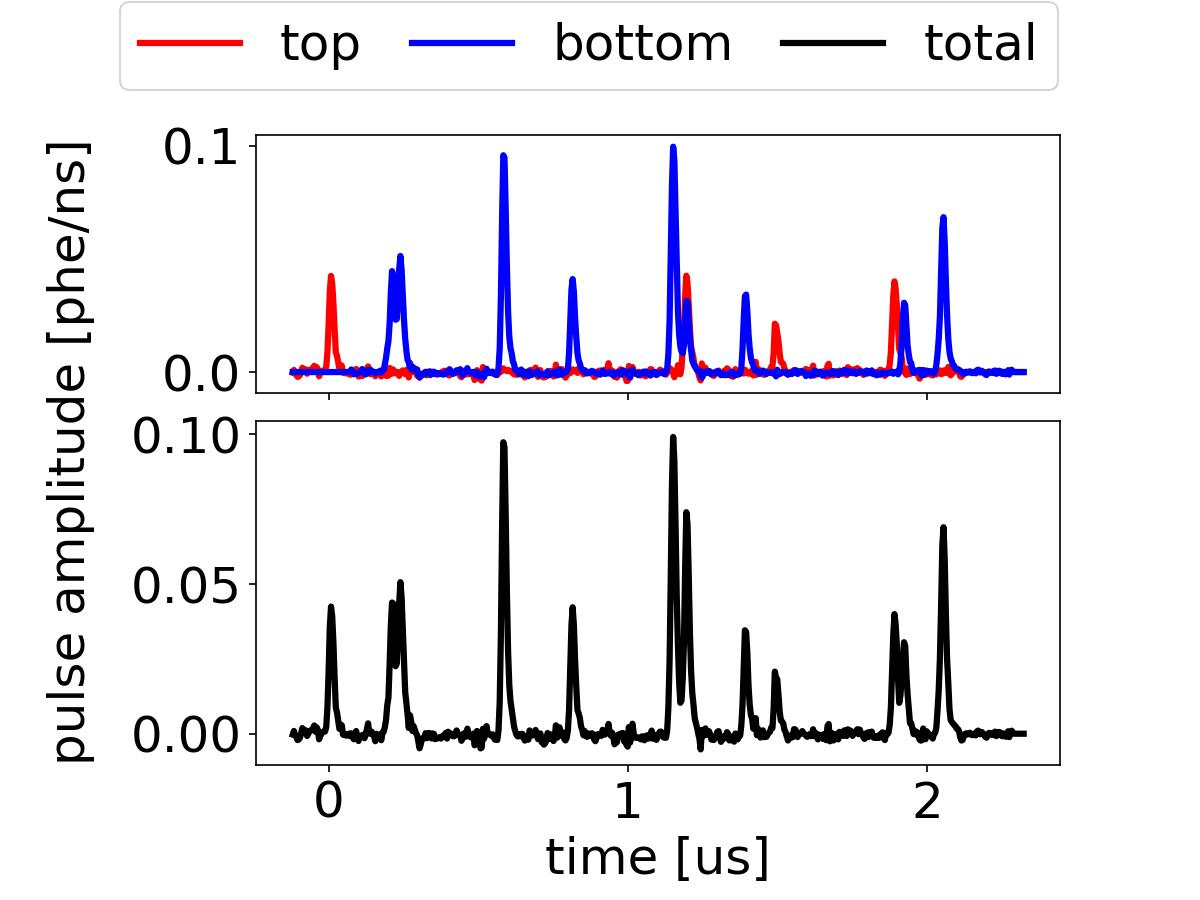
\includegraphics[width=\figurewidth,clip,trim={0 0 0 0}]{Figures/GasTest/exampleWaveforms/proc64767id00000197.jpg}%062
	\caption{}
	\label{fig:ElectronEmissionPulse c}
\end{subfigure}
	\caption[\gtest\ electron emission event from grid wires]{\gtest\ electron emission event from grid wires. (a) Cartoon of the process. (b) An example waveform. Data were taken at \ddtt{2017}{12}{08}{14}{02}, with \opvtvb\ at \SIlist{+6;-6}{kV}, \opgd\ at \standarddensity . See text for details.}
	\label{fig:ElectronEmissionPulse}
\end{figure}

Of the features described above, the most important features of  the \ees\ is the EL duration. The other signal shape features, such as the early and late gas gain peaks, are not apparent because the light collection efficiency is not high enough. The EL duration is approximately equal to the duration of electron drift between the two electrodes. The deviation of electric field between the two electrode is much smaller than its average value. Therefore, the drift duration can be roughly estimated by, 

\begin{align}
\text{drift duration} = \frac{\text{distance between two electrodes}}{\text{drift velocity at the average electric field between two electrodes} }
\end{align}

The other important feature of the \ees\ is the quantity of its EL production. EL light production in the major part of \ees\ is uniform, except for at the beginning and at the ending of the signal, because the deviation of the drift electric field is small. Since the electron multiplication around the cathodic wires happens early in the process before the major EL light production, the total counts of photons created in an \ees\  can be estimated as,
\begin{align}
\#\ \text{EL photons} & \approx \#\ \text{EL photons per drifted electron} \times \text{cathodic gas gain}
\end{align}
where the number of EL photons per drifted electron and the cathodic gas gain are estimated below.

The number of EL photons per drifted electron and the cathodic gas gain are related to the reduced electric field in the EL region and surface reduced electric field on the cathodic wire. The value of both reduced electric field can be derived from the gas density and the electric field, which can be estimated from the voltages, wire diameters and wire pitches of the two grids. The electrostatic solution of the electric field in the ELD is solved by COMSOL, as described in Appendix~\ref{chapter:field}. The results of the electric fields in the EL region (drift fields) and the average surface electric fields vs. \opdv\ are shown in Fig.~\ref{fig:surface electric field dV}.  The woven pattern of the grid cause that the surface electric field in the middle of the wire between two woven knots are higher than average by \SI{\sim 16}{\percent}, which is also discussed in Appendix~\ref{chapter:field}. The average number of photon production per EL distance is a known function of reduced electric field, as discussed in Section~\ref{sec:gtest light procduction}.% and its values at different \opgd\ and \opdv\ are shown in Fig.~\ref{fig:photon per drifted electron}. 
\begin{figure}[!htbp]
	\centering
	\begin{subfigure}[b]{0.8\textwidth}
		\centering
		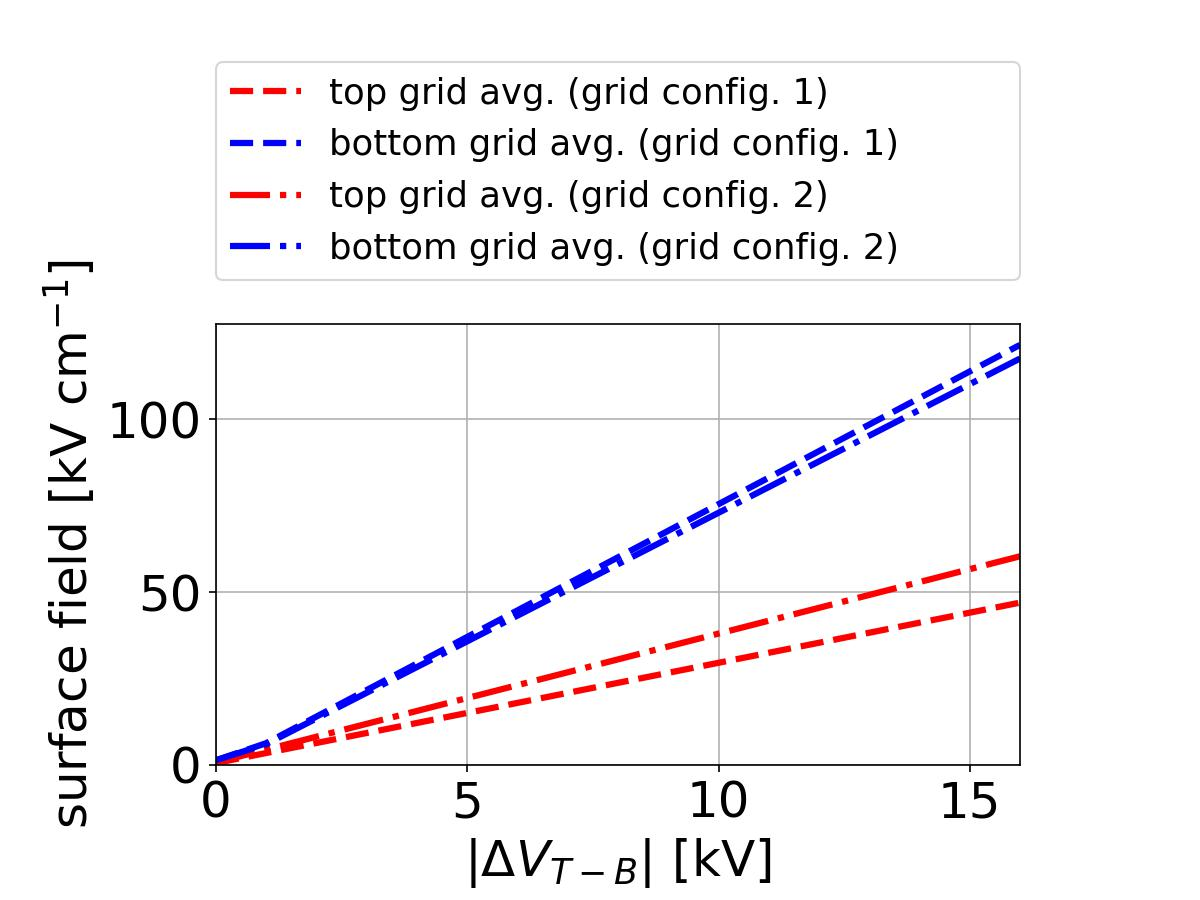
\includegraphics[width=\figurewidth,clip,trim={0 0 0 0},angle=0,origin=c]{Figures/GasTest/ElectricField/SurfaceElectricFieldGas.jpg}
		\caption[]{}
		\label{fig:surface electric field dV}
	\end{subfigure}
	\par\bigskip
	\begin{subfigure}[b]{0.8\textwidth}
		\centering
		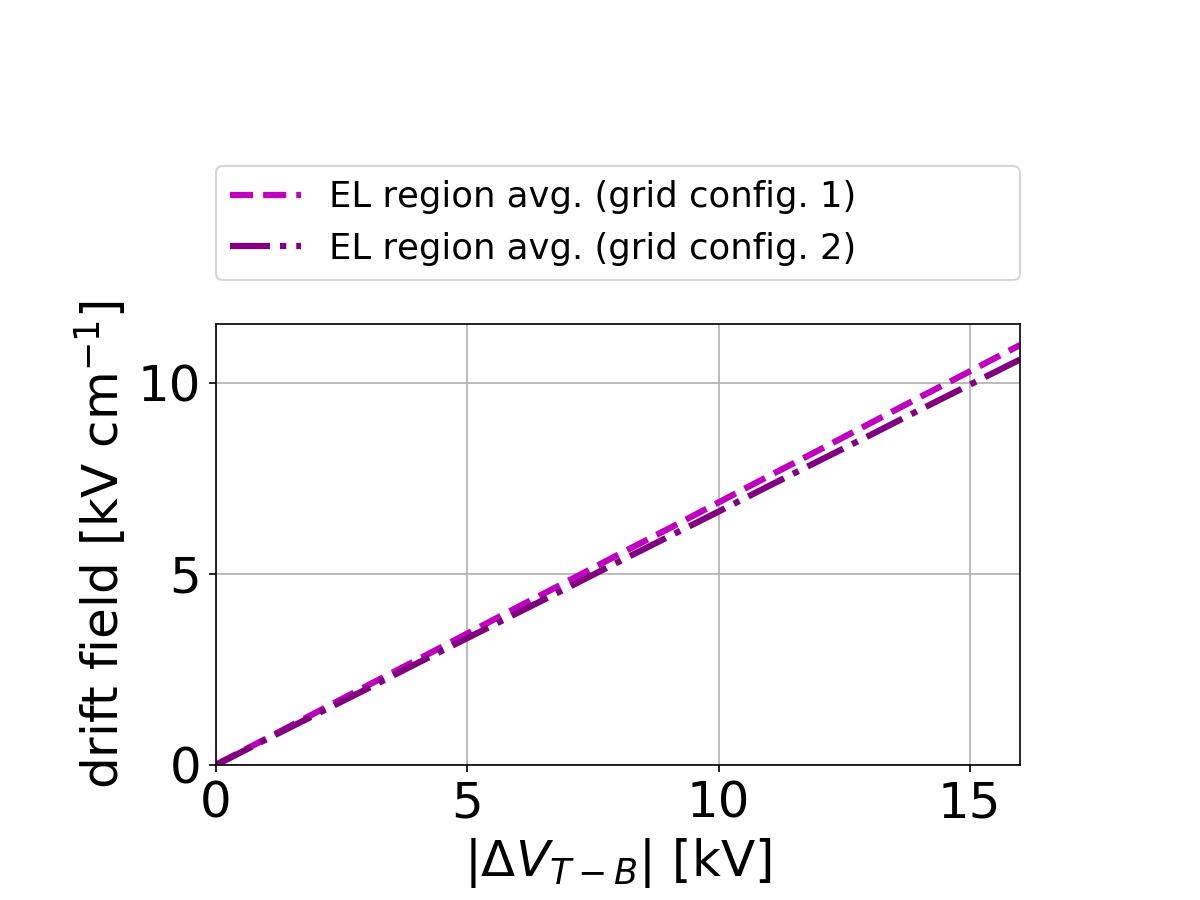
\includegraphics[width=\figurewidth,clip,trim={0 0 0 0}]{Figures/GasTest/ElectricField/DriftElectricFieldGas.jpg}
		\caption{}
		\label{fig:drift electric field dV}
	\end{subfigure}
	\caption[\gtest\ detector electric field.]{\gtest\ detector electric field. (a) \gtest\ wire surface electric field vs. \opdv\ for the top and bottom grid in different grid configurations. (b) \gtest\ EL region drift electric field vs. \opdv\ in different grid configurations.}
	\label{fig:gtest electric field}
\end{figure} %code in /Users/weiji/Google Drive/gastest/ElectricField

With the known surface reduced electric field, electron multiplication (cathodic gas gain) is studied using gas simulation softwares. A simple geometry is build and meshed in GMSH, as described in Ref.~\cite{Geuzaine2009}.  This software is capable of defining 3D finite element mesh, which interfaces with softwares like ElmerSolver and Garfield++ to solve the electric field in a defined geometry. Fig.~\ref{fig:electron multiplication sim geo} shows the defined geometry. This geometry includes a thin cylindrical surface in the center representing the grid wire as the surface emitting electrons, and a thick cylindrical surface outside representing the cut-off distance of electron multiplication. This cut-off distance is chosen to be sufficiently long so that the electric field beyond this distance is too small to allow most of the electron multiplication. The diameter of the two cylinders are \SI{75}{\um} and \SI{1}{\cm}. Voltages are assigned to two cylinders to create a chosen electric field on the surface of the wire. Next, the electric field map in this full geometry is solved by Elmer, as described in Ref.~\cite{Elmergrid2000, Kotila1999}.  Then, the gas simulation under such electric field map is done with Magboltz in Garfield++ interface, as described in Ref.~\cite{Biagi1999, Veenhof1998}. These softwares implement light yield and charge yield, also known as the photon and electron production, for electrons moving in a gas medium as a function of reduced electron field. By including the electric field map and choosing the corrects gas density, these softwares are able to simulate the photon and electron production with an electron that initiate from the wire surface. 

An example of electron multiplication simulation in the simple geometry is shown in Fig:~\ref{fig:electron multiplication sim result}. As the electron moves further away from the wire surface, both light production and electron production reduce. Results of the counts of electron multiplication vs. surface electric field at different gas density is shown in Fig.~\ref{fig:electron multiplication}. The number of collected EL photons of the \ees\ signals are shown in Fig.~\ref{fig:photon per electron sim}. Together with the EL duration, this number of collected EL photons are the important features of \ees\ signals that we used in the signal classification.
%Light collection of created photons also influence the total counts and duration of \ees . The approximately \SI{2}{\percent} light collection efficiency in the ELD results in only a portion of EL photons are seen by the PMTs. It causes the waveform of an \ees\ more coarsely distributed in time. This low number of collected photons also increases the difficulty of estimating the real EL duration.

\begin{figure}[!htbp]
	\centering
	\begin{subfigure}[b]{0.45\textwidth}
		\centering
		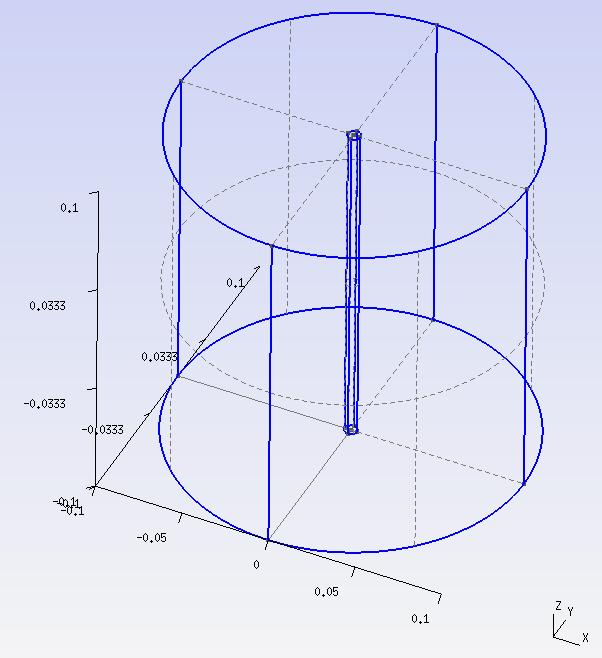
\includegraphics[width=\figurewidth,clip,trim={0 0 0 0}]{Figures/GasTest/GarfieldResults/SingleWireGeoPlus.jpg}
		\caption{}
		\label{fig:electron multiplication sim geo}
	\end{subfigure}
	\par\bigskip
	\begin{subfigure}[b]{\figurewidth}
		\centering
		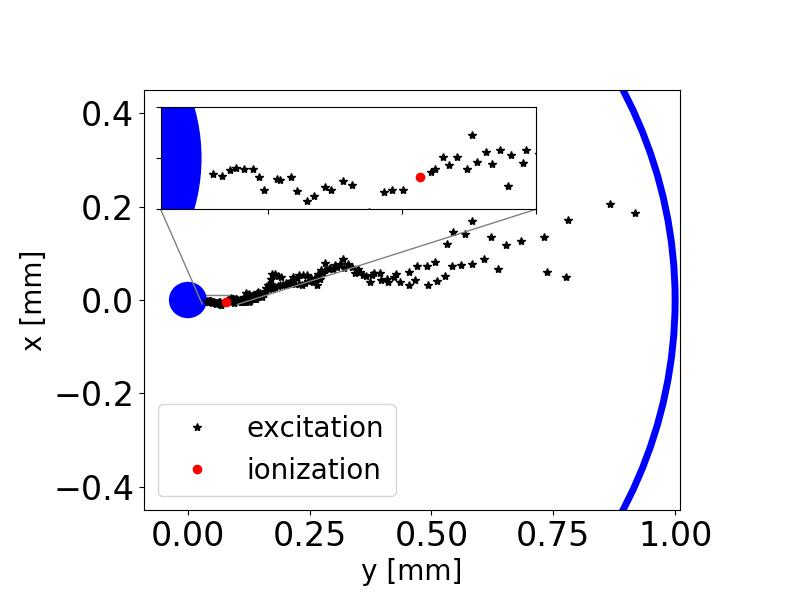
\includegraphics[width=\halfwidth,clip,trim={20 0 70 0}]{Figures/GasTest/GarfieldResults/GarOneEvent100.jpg}
		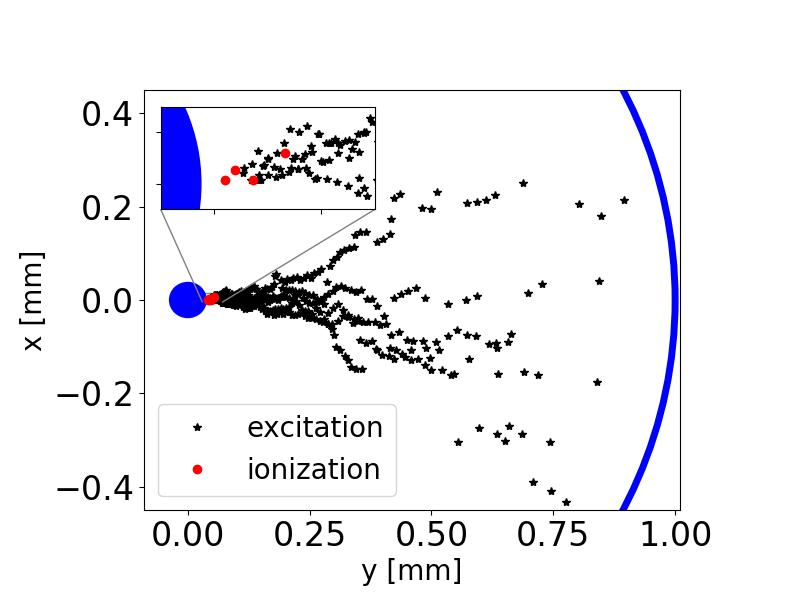
\includegraphics[width=\halfwidth,clip,trim={20 0 70 0}]{Figures/GasTest/GarfieldResults/GarOneEvent101.jpg}
		\caption{}
		\label{fig:electron multiplication sim result}
	\end{subfigure}
	\caption[A 3D simulation of an electron drifting in an axially symmetric electric field in xenon gas.]{A 3D simulation of an electron drifting in an axial symmetric electric field in xenon gas. (a) Geometry defined in GMSH (unit in \si{\cm}) \cite{Geuzaine2009}. Electrons are emitted at one point from the wire in the center. (b) Example simulation results, which is taken at \opgd\ \SI{0.137}{\mole\per\liter} (T = \SI{295}{\kelvin}, P = \SI{3.3}{\bara}), showing the excitation and ionization sites. The blue curves are the boundary of the outer edge of simulation (diameter : \SI{2}{\mm}) and  the wire surface (diameter: \SI{75e-3}{\mm}). Left: a simulated event with a single ionization site. Right: a simulated event with four ionization sites. This simulation is conducted with Elmer and Garfield++, as described in Ref.~\cite{Elmergrid2000, Kotila1999, Biagi1999, Veenhof1998}.}
	\label{fig:electron multiplication sim}
\end{figure}

\begin{figure}[!htbp]
	\centering
	\begin{subfigure}[b]{0.7\textwidth}
		\centering
		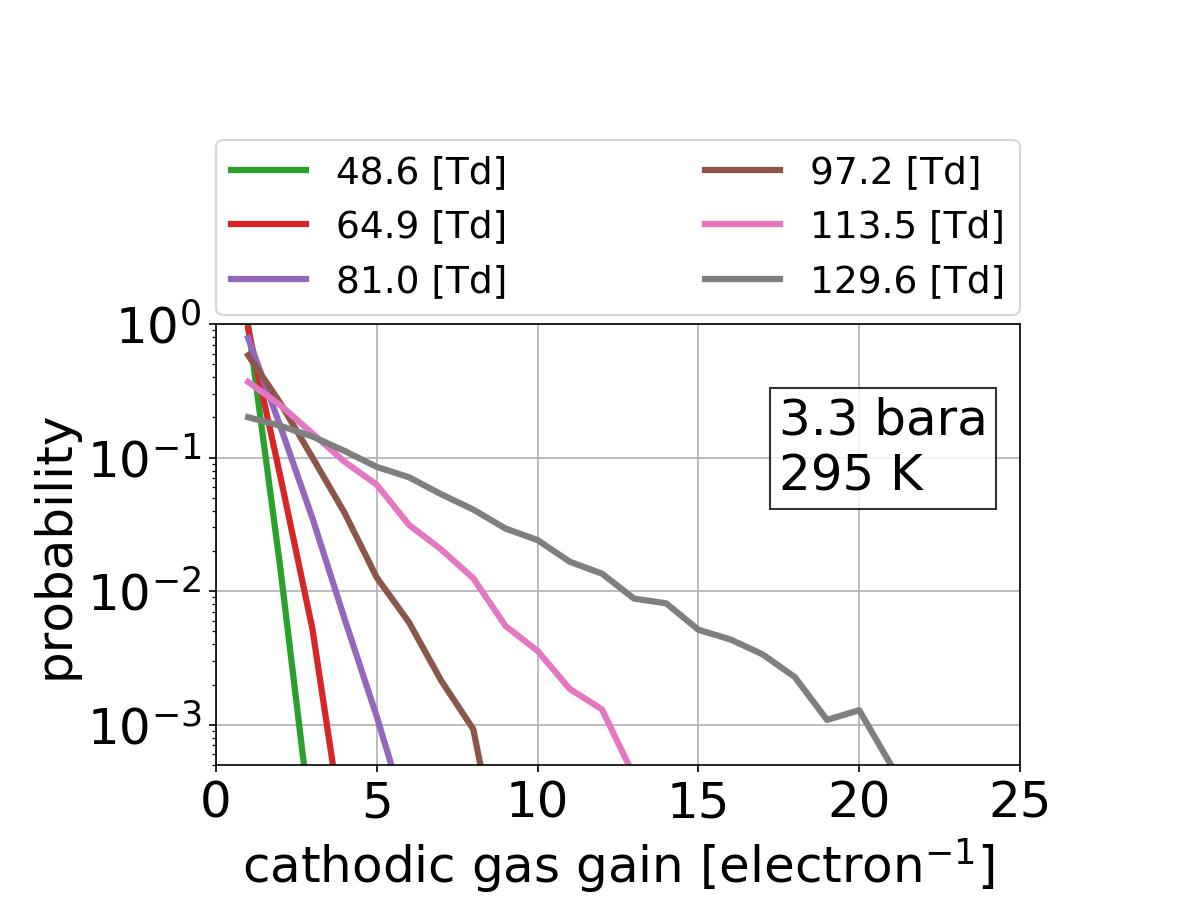
\includegraphics[width=\figurewidth,clip,trim={0 0 0 0}]{Figures/GasTest/xenonProperties/PhotonMultiplicationNaiveReduced.jpg}
		\caption{}
		\label{fig:electron multiplication ind}
	\end{subfigure}
%	\par\bigskip
	\begin{subfigure}[b]{0.7\textwidth}
		\centering
		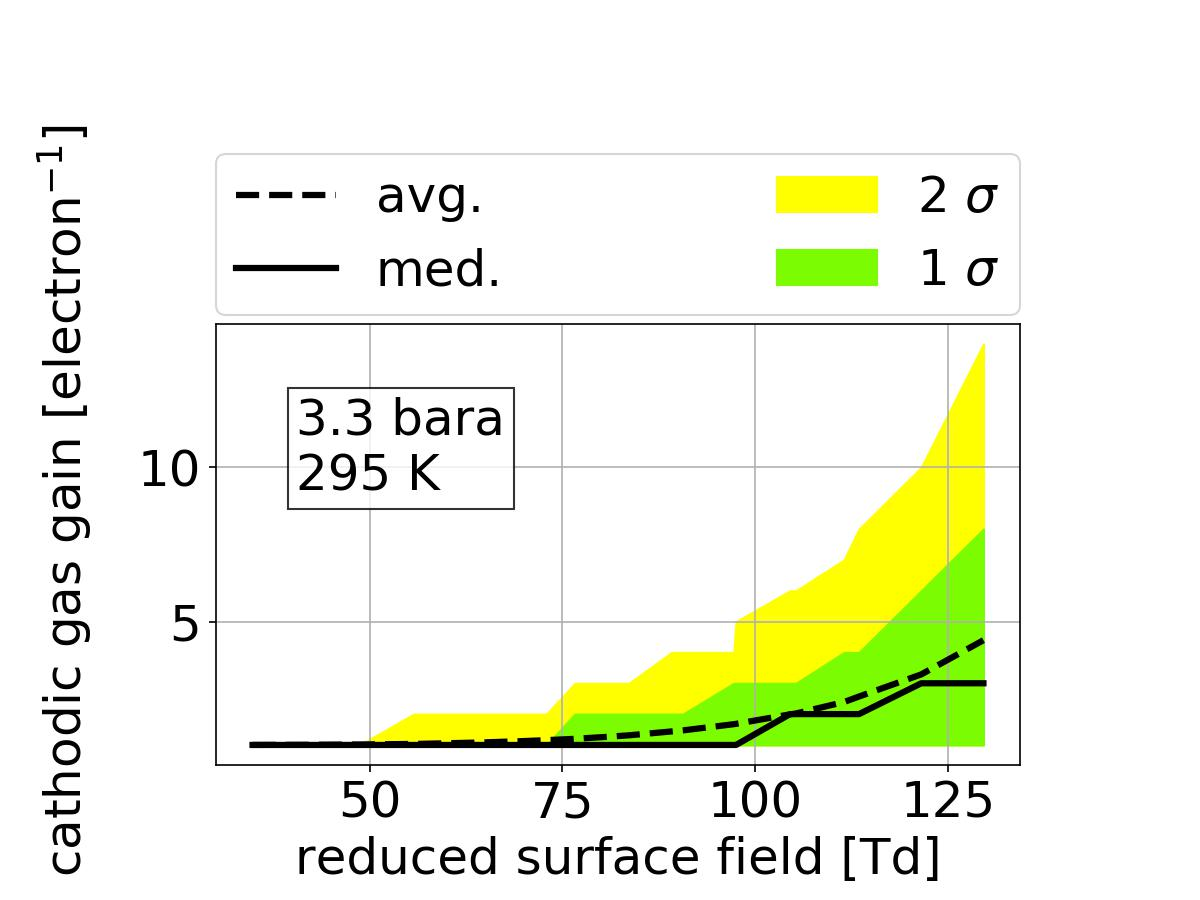
\includegraphics[width=\figurewidth,clip,trim={0 0 0 0}]{Figures/GasTest/xenonProperties/MultiplicationMeanSigma3300mbarReduced.jpg}
		\caption{}
		\label{fig:electron multiplication para}
	\end{subfigure}
	\caption[Simulated cathodic electron gas gain vs. reduced surface electric field.]{Simulated cathodic electron gas gain vs. reduced surface electric field. (a) Simulated cathodic gas gain probability distribution in different reduced surface electric fields. (b) The average, median, \onesigma\ band (\SIrange{15.9}{84.1}{\percent}), and \twosigma\ band (\SIrange{2.3}{97.7}{\percent}) of cathodic gas gain vs. the reduced surface electric field. Simulation is taken at \opgd\ \SI{0.137}{\mole\per\liter} (T = \SI{295}{\kelvin}, P = \SI{3.3}{\bara}).}
	\label{fig:electron multiplication}
\end{figure}% code in '/Users/weiji/Google Drive/gastest/xenonProperties/xenonIonization.py'

\begin{figure}[!htbp]
	\centering
	\begin{subfigure}[b]{0.7\textwidth}
		\centering
		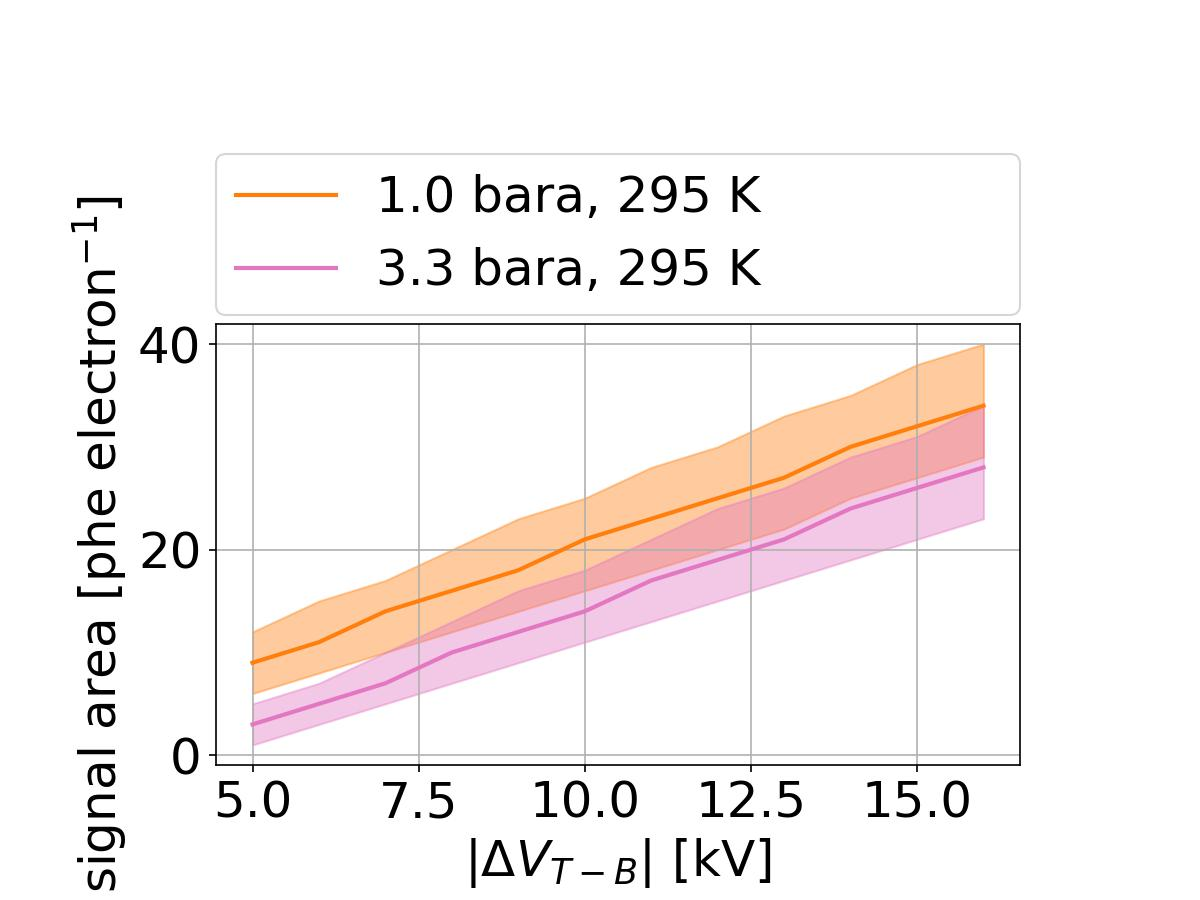
\includegraphics[width=\figurewidth,clip,trim={0 0 0 0}]{Figures/GasTest/xenonProperties/MultiplicationPhotonCollectionNaiveProfileMeanSigma3300mbarPerDriftElecton.jpg}
		\caption{}
		\label{fig:photon per drifted electron }
	\end{subfigure}
%	\par\bigskip
	\begin{subfigure}[b]{0.7\textwidth}
		\centering
		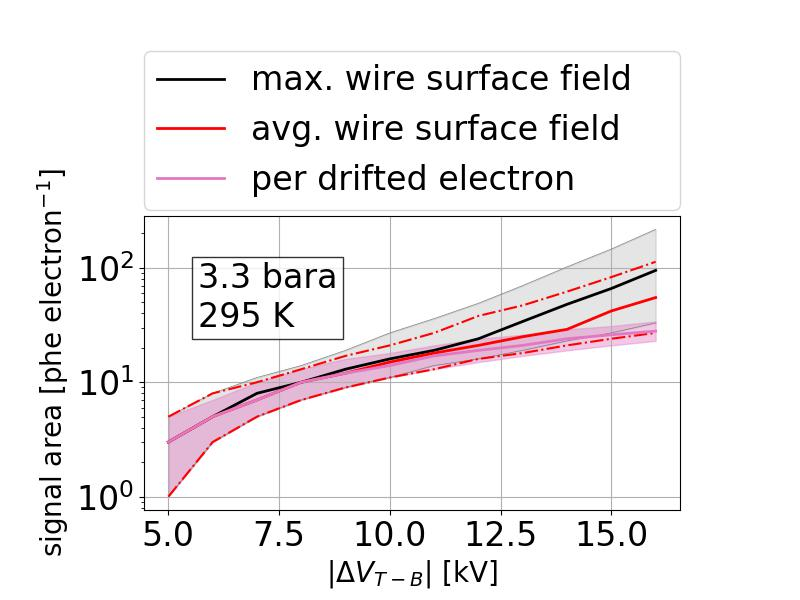
\includegraphics[width=\figurewidth,clip,trim={0 0 0 0}]{Figures/GasTest/xenonProperties/MultiplicationPhotonCollectionNaiveProfileMeanSigma3300mbar.jpg}
		\caption{}
		\label{fig:photon per electron}
	\end{subfigure}
	\caption[Simulated signal areas vs. \opdv .]{Simulated signal areas vs. \opdv . (a) Simulated signal area of a single drifted electron from the bottom grid at different gas densities. (b) Simulated signal area of an electron generated at different locations on the bottom grid. The black line corresponds to locations with maximum electric field on the grid. The red line corresponds to locations with average electric field on the grid. The green line shows the simulated signal area of a single drifted electron. Simulation is taken at \opgd\ \SI{0.137}{\mole\per\liter} (T = \SI{295}{\kelvin}, P = \SI{3.3}{\bara}). The solid lines are the medians. The dashed lines, color shaded bands are \onesigma\ bands (\SIrange{15.9}{84.1}{\percent}), respectively.}
	\label{fig:photon per electron sim}
\end{figure}% code in '/Users/weiji/Google Drive/gastest/xenonProperties/xenonIonization.py'

Therefore, \ees s  have a known EL duration and EL photons production dependence on the detector \opgd\ and \opdv . We use these two important characteristics of signals to distinguish \ees s in the future signal classification.

\subsection{Particle radiation}
\label{sec:events particle}
Particle radiation is the high energy particle originating from radioactive decay of unstable atoms in materials inside and outside the detector. The high energy particle enter the detector and deposit energy there through different processes. A high energy photon (gamma radiation) loses energy through thermal elastic scattering, photoelectric process, Compton scattering, and other particle energy loss processes; A high energy charged particle, e.g. electron (beta radiation), \ce{^{4}_{2}He} (alpha radiation), predominately loses it energy through ionizing atoms in detector materials, as described in Ref.~\cite{Blum2008}.  These processes produce excited xenon atoms and free electrons, which later produce primary scintillation and EL photons. The primary scintillation photons (S1) are collected and seen immediately. The EL photons, on the other hand, resulting from electrons drifting in the high electric field region in the detector, are usually produced later. 

A high energy gamma event can enter the ELD since its energy loss in detector skin materials is small. The photon attenuation length, which characterizes how far a photon can go, usually decrease as we have denser materials, higher average atomic mass in the materials, and lower incident particle energy. The photon attenuation length in xenon is shown in Fig.~\ref{fig:xenon photon attenuation}. Along photon attenuation, high energy electrons can be produced from gamma radiation through some kind of energy loss process, like Compton scattering, Auger electron emission. These high energy electrons can be produced inside the ELD, deposit its energy, and raise signals in the detector. The energy deposition length depends on the material, especially its density and its average atomic mass, and the energy of the incident particle. Similar to the photon attenuation process, denser material, higher average atomic mass, and lower incident particle energy usually results in smaller energy deposition length. The energy deposition length in xenon is shown in Fig.~\ref{fig:xenon electron range}. For an electron with energy in the range of \SIrange{10}{1000}{\keV}, which is the common energy for beta radiation, the continuous slowing down approximation range (CSDA range), also know as the average path length traveled by the charged particle (electron), is in the range of \SIrange{6e-4}{1}{\gram\per\cm\squared}, corresponding to \SIrange{1e-5}{2.e-2}{\cm} with xenon gas density at \standarddensity\ (\SI{18.0e-3}{\gram\per\cm\cubed}). %This energy deposition length is smaller compared to the height of the EL region, indicating low possibility for distinguishing the by arrival time of the secondary electrons.
The number of free ionization electrons in this event is associated with the energy-loss of the incident particle. During the measurement, a population associated with xenon K shell X-ray ($K_{\alpha}$: \SI{29.8}{\keV}, $K_{\beta}$: \SI{33.6}{\keV}, from Ref.~\cite{Dulieu2007, TabRadv8}) is observed to be one of the byproduct of particle radiation energy loss process, confirming that this type of signal is associated with external radiation.

\begin{figure}[!htbp]
	\centering
	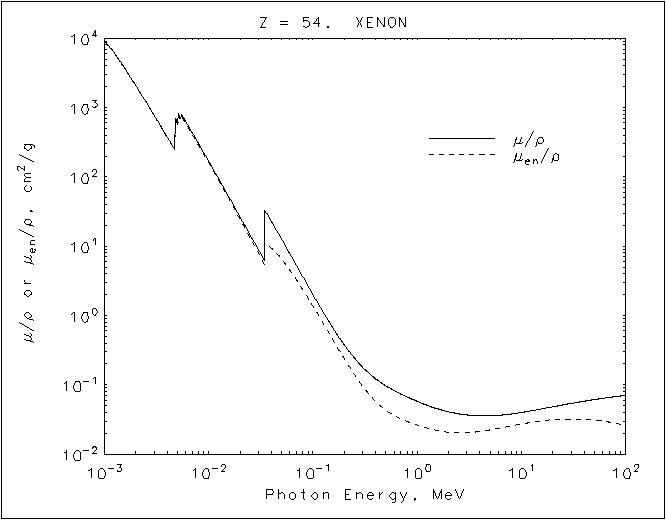
\includegraphics[width=.7\textwidth,clip,trim={0 0 0 0},angle=0,origin=c]{Figures/GasTest/XenonPhysicsUseful/PhotonAttenuation.jpg}
	\caption[Attenuation length of photon in xenon.]{Attenuation length of photon in xenon, from Ref.~\ref{NIST,}.}
	\label{fig:xenon photon attenuation}
\end{figure}

\begin{figure}[!htbp]
	\centering
	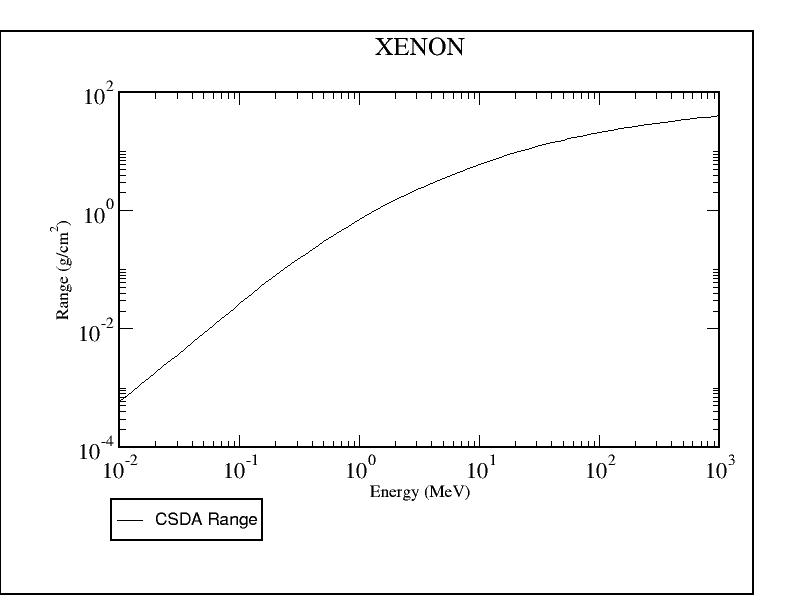
\includegraphics[width=.7\textwidth,clip,trim={0 0 0 0},angle=0,origin=c]{Figures/GasTest/XenonPhysicsUseful/ElectronRange.jpg}
	\caption[CSDA range of electrons in xenon.]{CSDA range of electrons in xenon, from Ref.~\ref{NIST, ESTAR}.}
	\label{fig:xenon electron range}
\end{figure}

A high energy external beta radiation, however, is less likely to enter the ELD compared to high energy gamma radiation because the beta radiation penetration length (approximate to the material CDSA range) is shorter than gamma radiation. Since the electron CDSA range is small compared to the thickness of xenon gas skin outside the ELD, with addition stopping power from dense PTFE reflector cone, the beta radiation would be stopped before it enters the ELD. 

According to the location of energy deposition site, the high energy particle from radiation produce different look of signals, which will be discussed separately.

\paragraph{Anode cone event} 
\label{sec:events particle anode cone}
Anode cone events are the particle radiation events which have energy deposition location in the PTFE reflector cone close to the anodic grid side (anode cone). A cartoon of the physical process and an example waveform of anode cone event, as well as two zoomed plots of the waveform in different parts of the process, are shown in Fig.~\ref{fig:anode cone}. The cartoon part A in Fig.~\ref{fig:anode cone a} shows an external particle entering the anode cone region and deposit energy there. This process produce scintillation photons, the signal of which are collected and seen immediately, shown in Fig.~\ref{fig:anode cone d}. The primary scintillation signal normally has a TBA (top-bottom asymmetry) heavier in the anode side PMT than the cathode side, indicating this photon signal is produced in the anode cone (top cone in this case). The free electrons drift to the anodic grid according to the electric field in the anode cone . Even though the electric field in the cone region is too small to produce large quantity of EL light during electron drift, when these electrons get close to the anodic grid wire, the electric field around the anodic grid wires are big enough to produce EL light. This is the source of the secondary photon signal, which follows the preceding signal after the amount of time that it took electron to drift. The cartoon part B in Fig.~\ref{fig:anode cone b} shows this process, and Fig.~\ref{fig:anode cone e} shows the corresponding part of the signal. The pulse shape of the secondary photon signals has a comparably slower rising and falling edge at the beginning and the ending of it. It also has a higher TBA because EL around the anode wire primarily happens above the anodic wire. The bottom PMT is in the shadow of grid wires when the top PMT is not. This difference causes a ratio of \num{\sim 2} increment on light collection ratio between the top PMT and the bottom PMT. These characteristic signatures are useful for veto large-area anode cone events. However, when their signal area get smaller (probably because of a lower energy deposition of external particles), it becomes difficult to find these signals by their shape. Therefore, a signal selection based on preceding signal is conducted to find the secondary signal from the primary scintillation signal. The time separation between these two signal is estimated by the known measured electron drift velocity in gaseous xenon, as described in Ref.~\ref{English1953, Brooks1982}. Electron drift velocity in gaseous xenon is approximately \SI{0.556}{\mm\per\us\per\townsend} E/N for reduced electric field (E/N) in the range of \SIrange{5}{25}{\townsend}. The maximum separation time for this detector at xenon gas density \standarddensity , \opvt\ in the range of \SIrange{+4}{+8}{\kV} is approximately \SIrange{85}{75}{\us}. The value of this maximum separation time decreases as decreasing the operation pressure in the detector. The value of maximum separation time drives the choice of \SI{100}{\us} preceding signal selections of this type of signals.  

\begin{figure}[!htbp]
	\centering
	\begin{subfigure}[b]{0.8\textwidth}
		\centering
		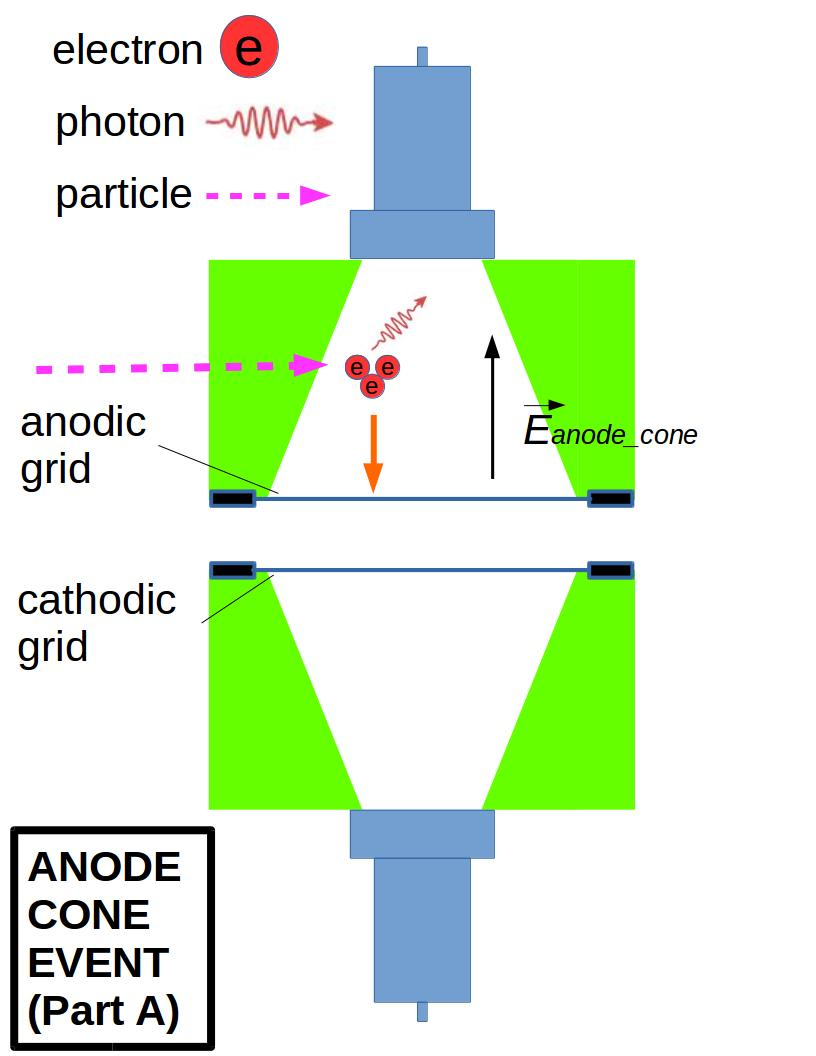
\includegraphics[width=\halfwidth,clip,trim={0 0 0 0},angle=0,origin=c]{Figures/GasTest/WeiDrawEvent/AboveAnoA.jpg}
%		\caption{}
%		\label{fig:anode cone a}
%	\end{subfigure}
%	\begin{subfigure}[b]{\halfwidth}
%		\centering
		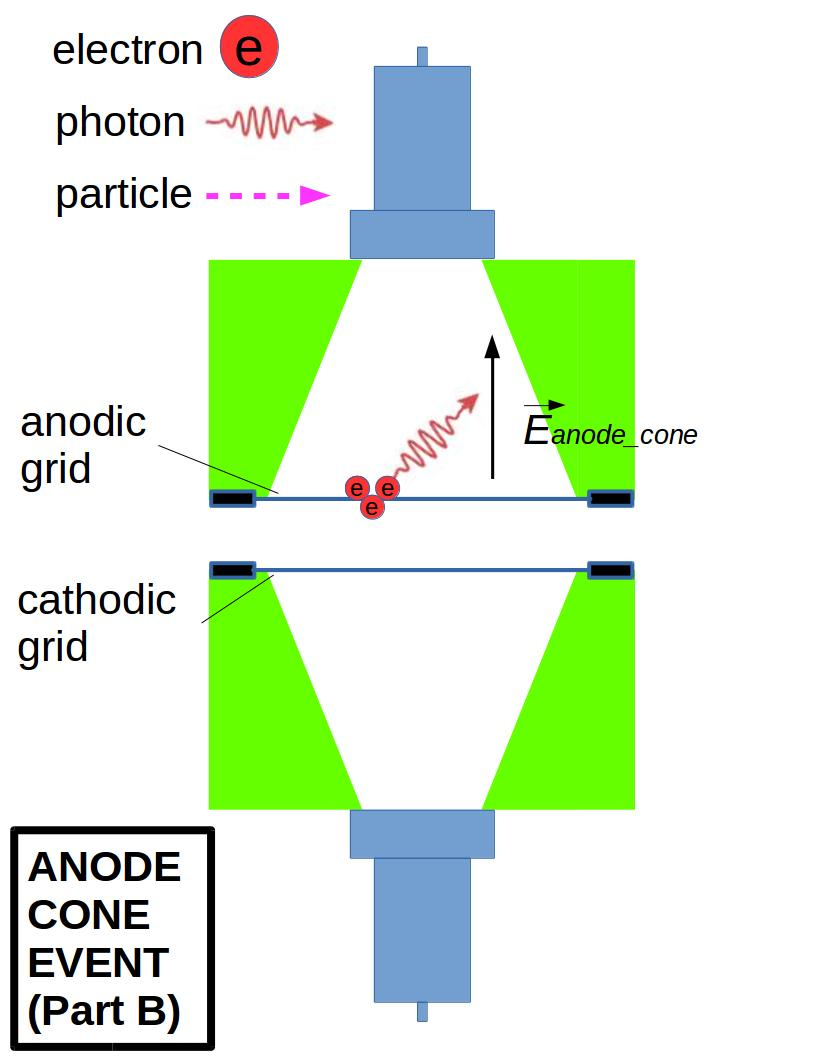
\includegraphics[width=\halfwidth,clip,trim={0 0 0 0}]{Figures/GasTest/WeiDrawEvent/AboveAnoB.jpg}
		\caption{}
		\label{fig:anode cone b}
	\end{subfigure}
	\par\bigskip
	\begin{subfigure}[b]{0.7\textwidth}
		\centering
		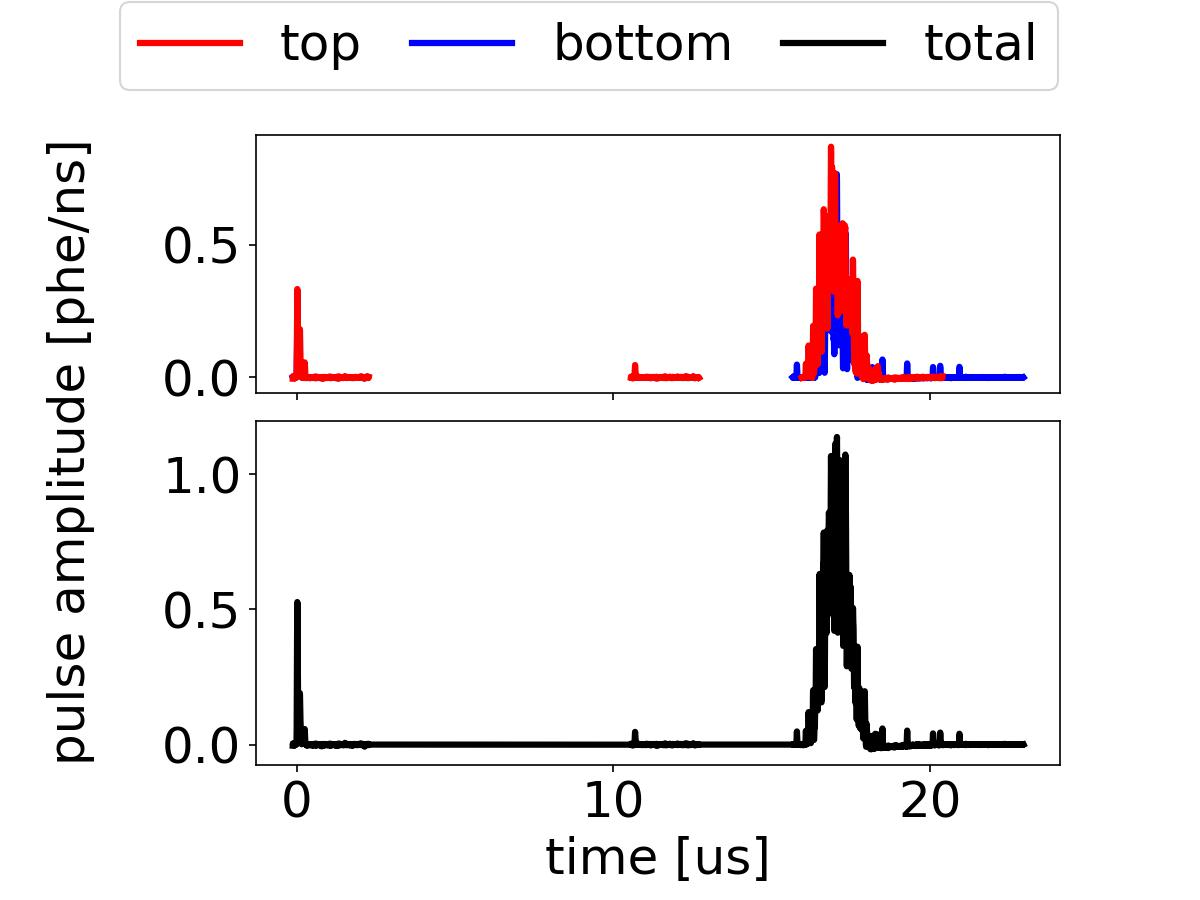
\includegraphics[width=\figurewidth,clip,trim={0 0 0 0}]{Figures/GasTest/exampleWaveforms/proc64767AnodeCone1.jpg}
		%{Figures/GasTest/exampleWaveforms/proc64767id00000047.jpg}
		\caption{}
		\label{fig:anode cone c}
	\end{subfigure}
	\caption[\gtest\ signal: anode cone event.]{\gtest\ signal: anode cone event. (a) Cartoon of the process. Left: Primary scintillation light  ionization electrons are produced from the particle interaction, and the ionization electrons drift to the anodic grid (part A). Right: EL light is produced in the high electric field region around the anodic grid wires (part B). (b) An example waveform of an anode cone event. Data were taken at \ddtt{2017}{12}{08}{14}{02}, with \opvtvb\ at \SIlist{+6;-6}{kV}, \opgd\ at \standarddensity .}
	\label{fig:anode cone}
\end{figure}

\begin{figure}[!htbp]\ContinuedFloat
	\centering
	\begin{subfigure}[b]{0.7\textwidth}
		\centering
		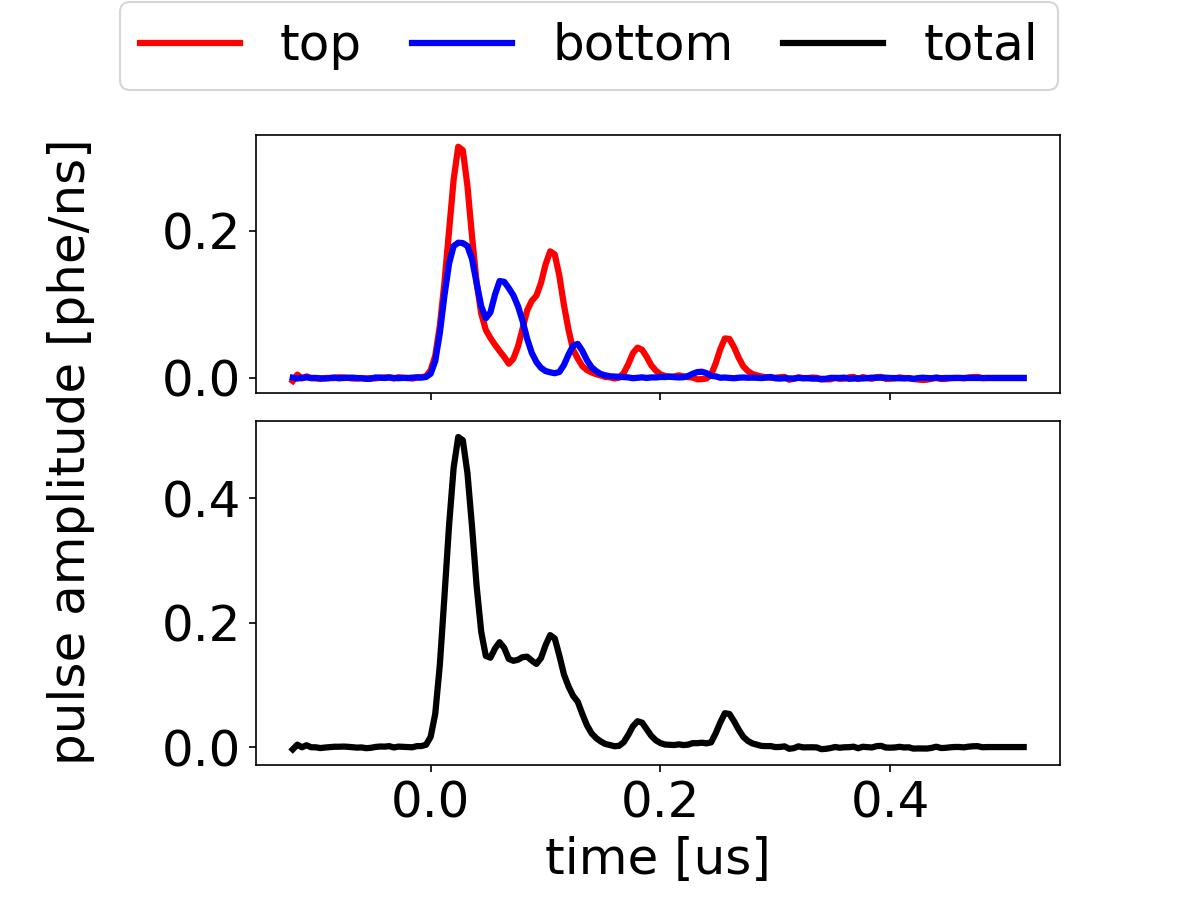
\includegraphics[width=\figurewidth,clip,trim={0 0 0 0}]{Figures/GasTest/exampleWaveforms/proc64767AnodeCone1P1.jpg}
		\caption{}
		\label{fig:anode cone d}
	\end{subfigure}
	\par\bigskip
	\begin{subfigure}[b]{0.7\textwidth}
		\centering
		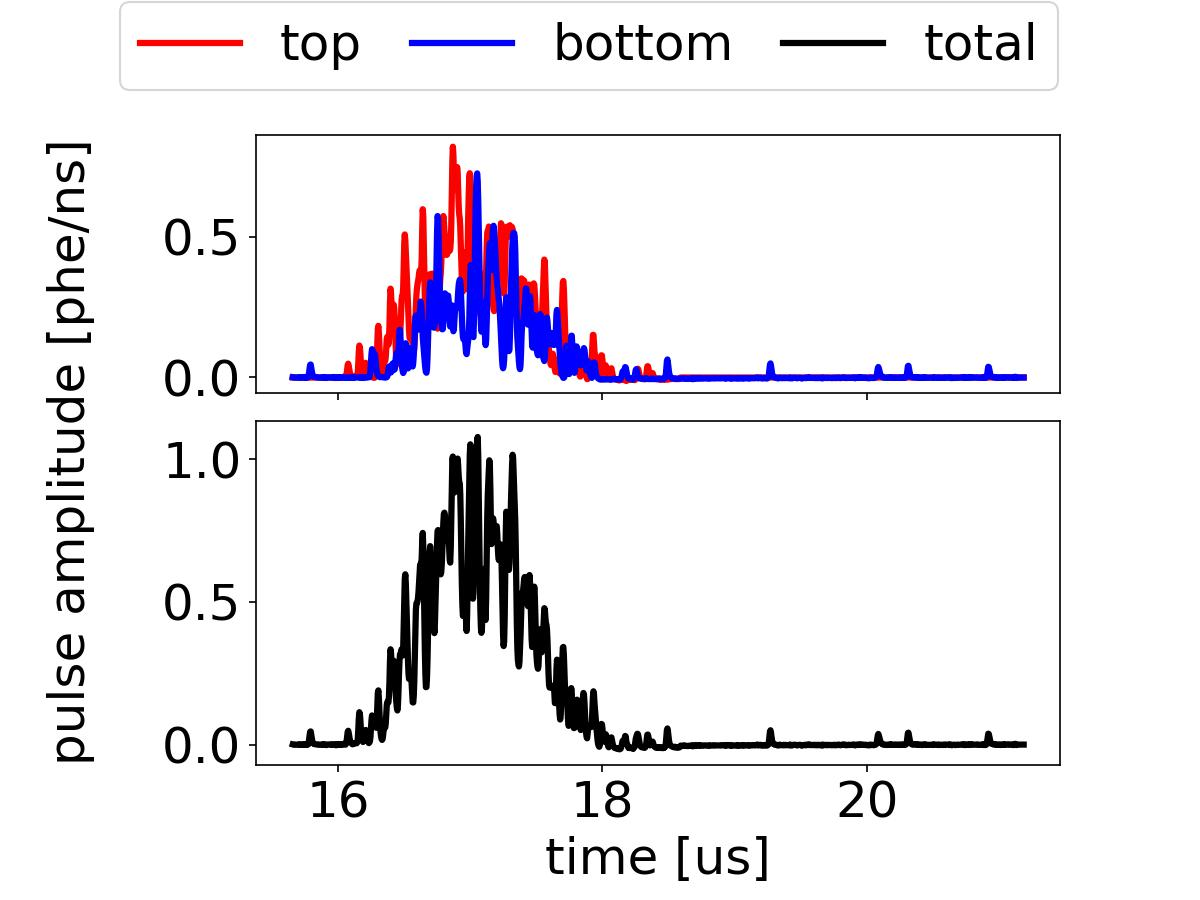
\includegraphics[width=\figurewidth,clip,trim={0 0 0 0}]{Figures/GasTest/exampleWaveforms/proc64767AnodeCone1P2.jpg}
		\caption{}
		\label{fig:anode cone e}
	\end{subfigure}
	\caption[\gtest\ signal: anode cone event (cont.).]{\gtest\ signal: anode cone event (cont.). (c) An example waveform of an anode cone event, zoomed in the range of \SIrange{0}{0.5}{\us}, which shows the primary scintillation light (cartoon part A). (d) An example waveform of an anode cone event, zoomed in the range of \SIrange{15}{21}{\us}, which shows the EL light produced around the anodic grid wires (cartoon part B). }
	\label{fig:anode cone cont}
\end{figure}

%This background from the secondary photon signals in anode cone events has a different pulse shape from \ees . 

%Thus, this cut is performed.  
\paragraph{Cathodic cone event}
\label{sec:events particle cathode cone}
Cathode cone events are the particle radiation events which have energy deposition location in the PTFE reflector cone close to the cathodic grid side (cathode cone). A cartoon of the physical process and an example waveform of cathode cone event are shown in Fig.~\ref{fig:cathode cone}. Similar to anode cone events, this process produce scintillation photons. However, the ionization electrons produced drift to cathode PMT. Therefore, EL light typically is produced during along their trajectories because the electric field in such region is much lower than the EL threshold. The primary scintillation signal normally has a TBA heavier in the cathode side PMT than the anode side PMT, indicating this photon signal is produced in the cathode cone (bottom cone in this case), as expected.

\begin{figure}[!htbp]
	\centering
	\begin{subfigure}[b]{0.8\textwidth}
		\centering
		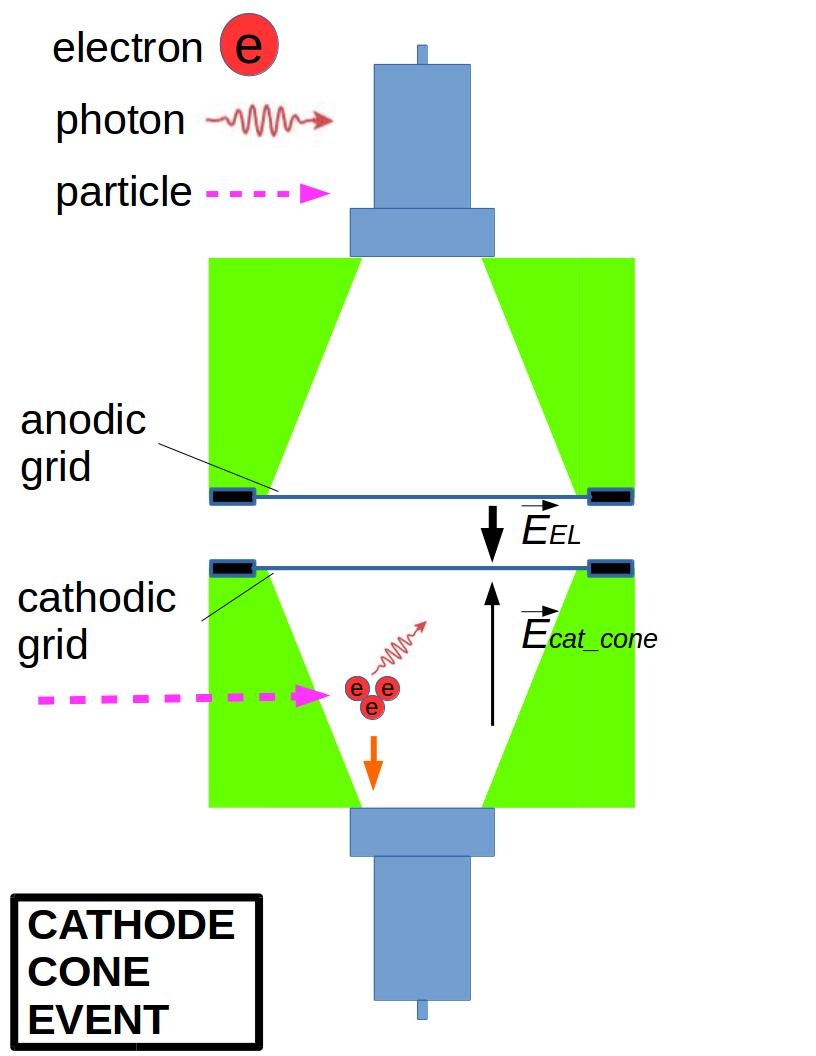
\includegraphics[width=\halfwidth,clip,trim={0 0 0 0},angle=0,origin=c]{Figures/GasTest/WeiDrawEvent/BelowCat.jpg}
		\caption{}
		\label{fig:}
	\end{subfigure}
	\par\bigskip
	\begin{subfigure}[b]{0.7\textwidth}
		\centering
		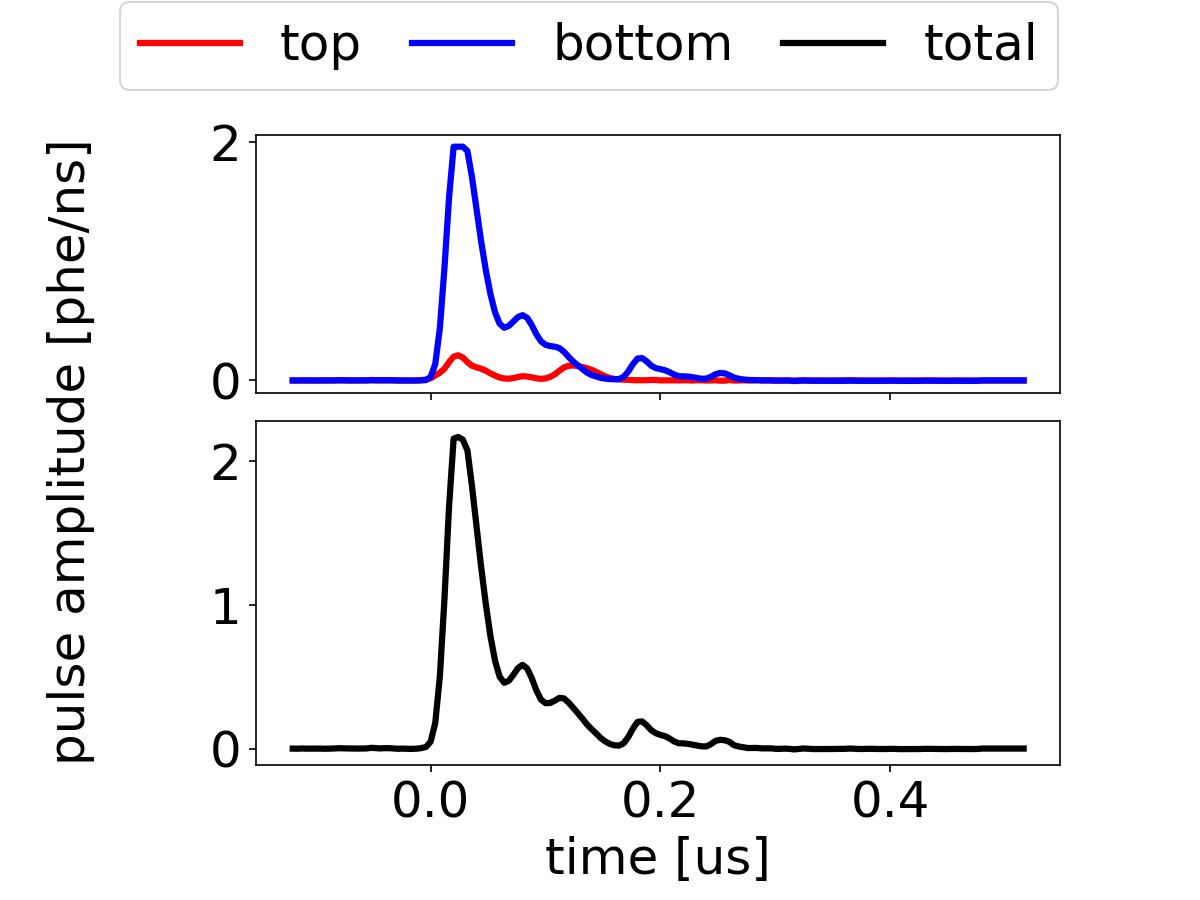
\includegraphics[width=\figurewidth,clip,trim={0 0 0 0}]{Figures/GasTest/exampleWaveforms/proc64767id00000021.jpg}%{Figures/GasTest/CutsValid/wave/testproc65831coinid0.jpg}
		\caption{}
		\label{fig:}
	\end{subfigure}
	\caption[\gtest\ signal: cathode cone event.]{\gtest\ signal: cathode cone event. (a) Cartoon of the process. Primary scintillation light ionization electrons are produced from the particle interaction, and the ionization electrons drift toward the bottom PMT. EL light is typically not produced along the trajectories of the electrons because the electric field in such region is lower than the EL threshold. (b) An example waveform of a cathode cone event. Data were taken at \ddtt{2017}{12}{08}{14}{02}, with \opvtvb\ at \SIlist{+6;-6}{kV}, \opgd\ at \standarddensity .%Data were taken at \ddtt{2018}{03}{12}{11}{41} , with \opvtvb\ at \SI{0}{\kV}, \opgd\ at vacuum.
		% proc13001, procid:101001, Aude rename the dataset name, really confusing now.	
	}
	\label{fig:cathode cone}
\end{figure}

\paragraph[]{S1 S2 event in the cathode corner}
\label{sec:events particle cathode corner}
S1 S2 events in the cathode corner (cathode corner events) are the particle radiation events which have energy deposition location either outside EL region and very close to the cathodic grid or in the corner between the cathodic grid and the cathodic cone. A cartoon of the physical process and an example waveform of cathode corner event are shown in Fig.~\ref{fig:cathode corner}. Similar to anode cone events, this process produce scintillation photons, which is shown in Fig.~\ref{fig:cathode corner b} (left) and the waveform of which is shown in the first \SI{0.3}{\us} in Fig.~\ref{fig:cathode corner c}. Since the free electrons produced in this event is really close to the cathode grid, according to electrostatic study using COMSOL software described in Ref.~\cite{COMSOL2018}, these electrons drift to cathodic grid, pass it, then drift in the EL region, the process of which produces EL photons along the trajectories of the electrons, and finally land on the anodic grid. This EL light production process is illustrated in Fig. ~\ref{fig:cathode corner b} (right), which corresponds to the waveform after \SI{0.5}{\us} in Fig.~\ref{fig:cathode corner c}. The static electric field from COMSOL solution is shown in Fig.~\ref{fig:gtest Comsol cathode corner}. Both the primary scintillation signal  and the secondary EL signal has a balanced TBA, indicating these photon signals are produced either in or really close to the EL region. 

\begin{figure}[!htbp]
	\centering
	\begin{subfigure}[b]{0.8\textwidth}
		\centering
		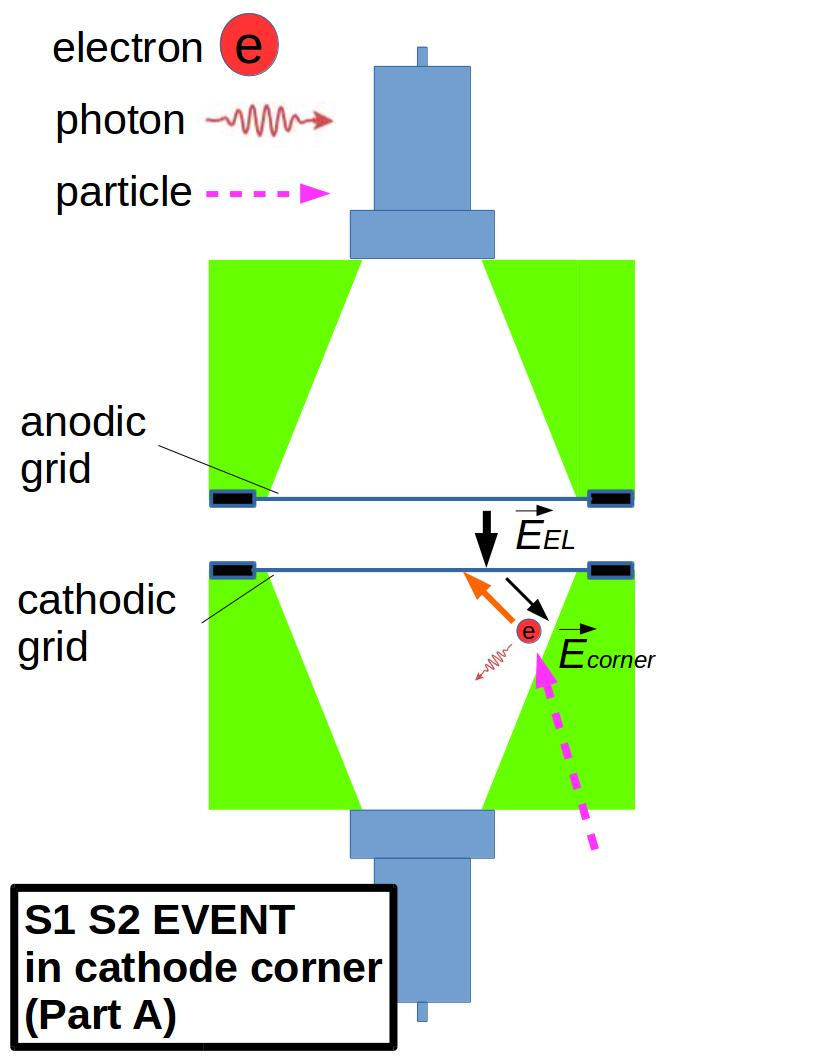
\includegraphics[width=\halfwidth,clip,trim={0 0 0 0},angle=0,origin=c]{Figures/GasTest/WeiDrawEvent/S1S2A.jpg}
%		\caption{}
%		\label{fig:cathode corner a}
%	\end{subfigure}
%	\begin{subfigure}[b]{\halfwidth}
%		\centering
		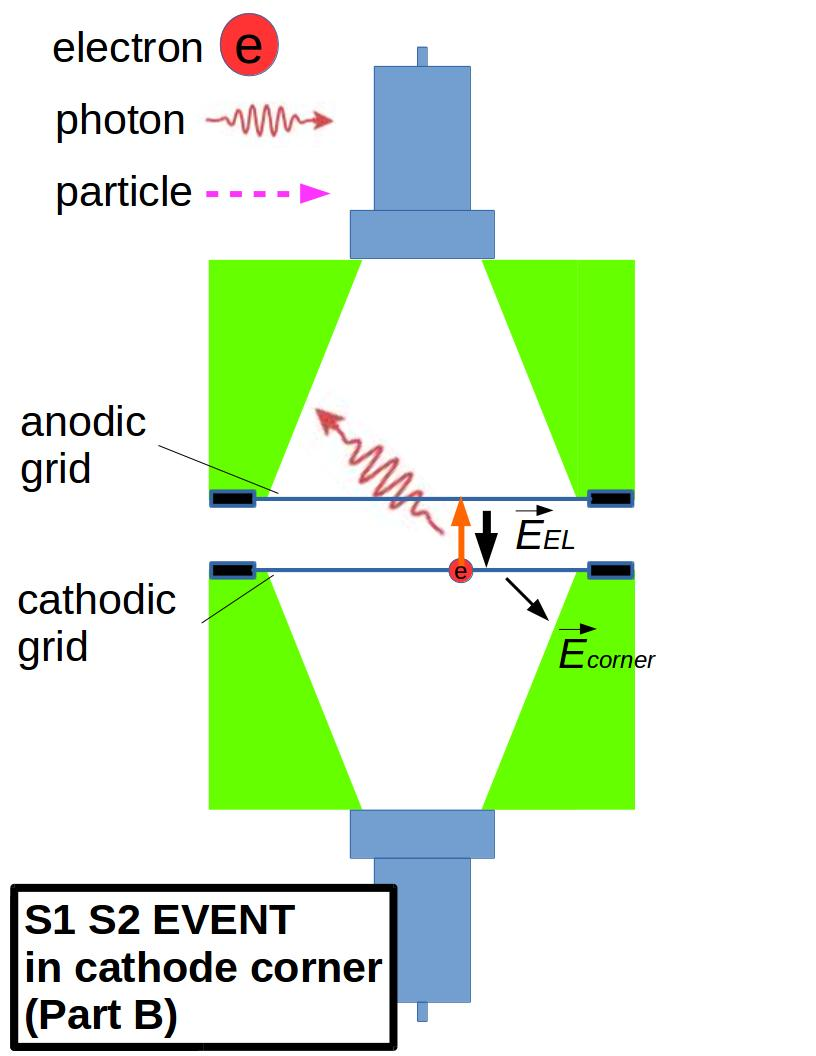
\includegraphics[width=\halfwidth,clip,trim={0 0 0 0},angle=0,origin=c]{Figures/GasTest/WeiDrawEvent/S1S2B.jpg}
		\caption{}
		\label{fig:cathode corner b}
	\end{subfigure}
	\par\bigskip
	\begin{subfigure}[b]{0.7\textwidth}
		\centering
		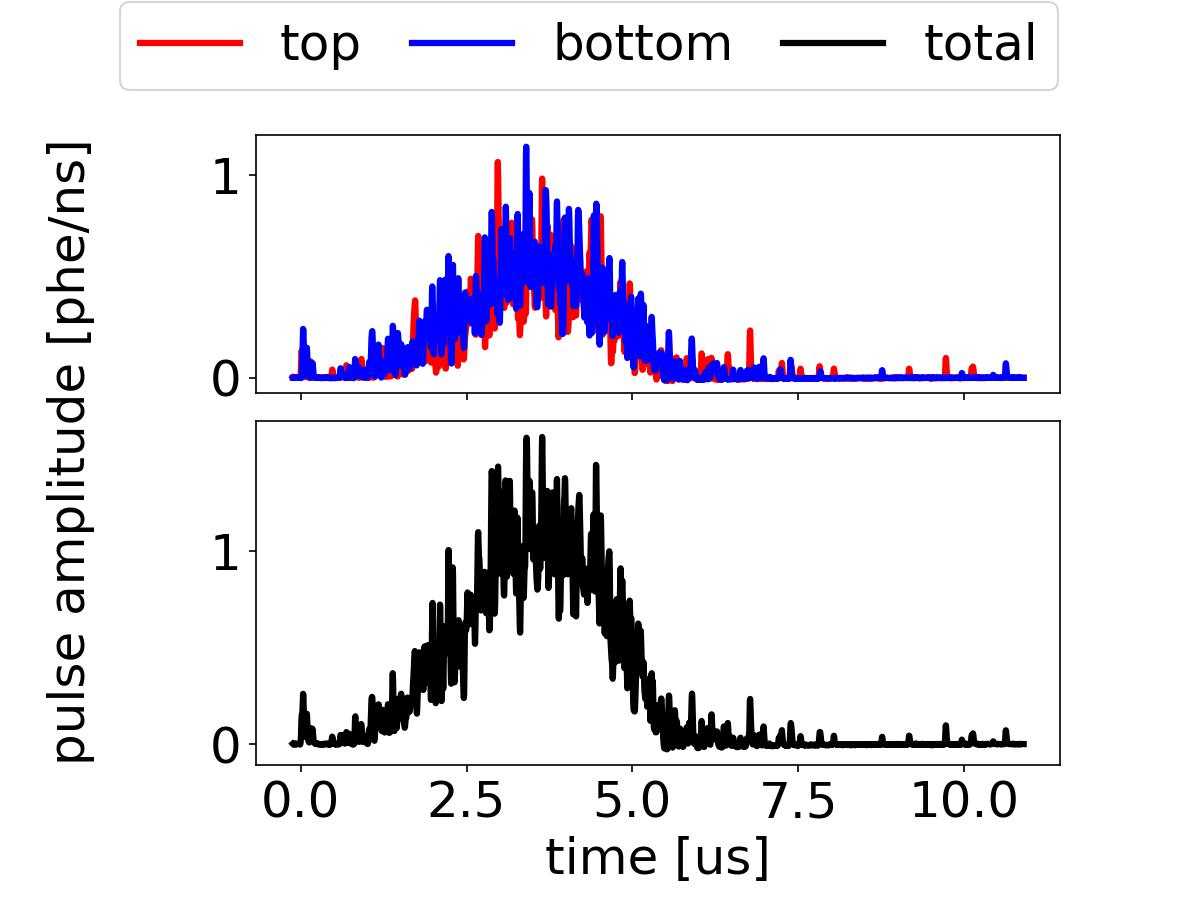
\includegraphics[width=\figurewidth,clip,trim={0 0 0 0}]{Figures/GasTest/exampleWaveforms/proc64767id00000145.jpg}%{Figures/GasTest/CutsValid/wave/testproc65831coinid0.jpg}
		\caption{}
		\label{fig:cathode corner c}
	\end{subfigure}
	\caption[\gtest\ signal: S1 S2 event in the cathode corner.]{\gtest\ signal: S1 S2 event in the cathode corner. (a) Cartoon of the process. Left: Primary scintillation light and ionization electrons are produced from the particle interaction, and the ionization electrons drift to the cathodic grid (part A). Right: EL light is produced in the EL region during electrons drifting to the anodic grid (part B). (b) An example waveform of an S1 S2 event in the cathode corner. Data were taken at \ddtt{2017}{12}{08}{14}{02}, with \opvtvb\ at \SIlist{+6;-6}{kV}, \opgd\ at \standarddensity .%Data were taken at \ddtt{2018}{03}{12}{11}{41} , with \opvtvb\ at \SI{0}{\kV}, \opgd\ at vacuum.
		% proc13001, procid:101001, Aude rename the dataset name, really confusing now.	
	}
	\label{fig:cathode corner}
\end{figure}

\begin{figure}[!htbp]
	\centering
	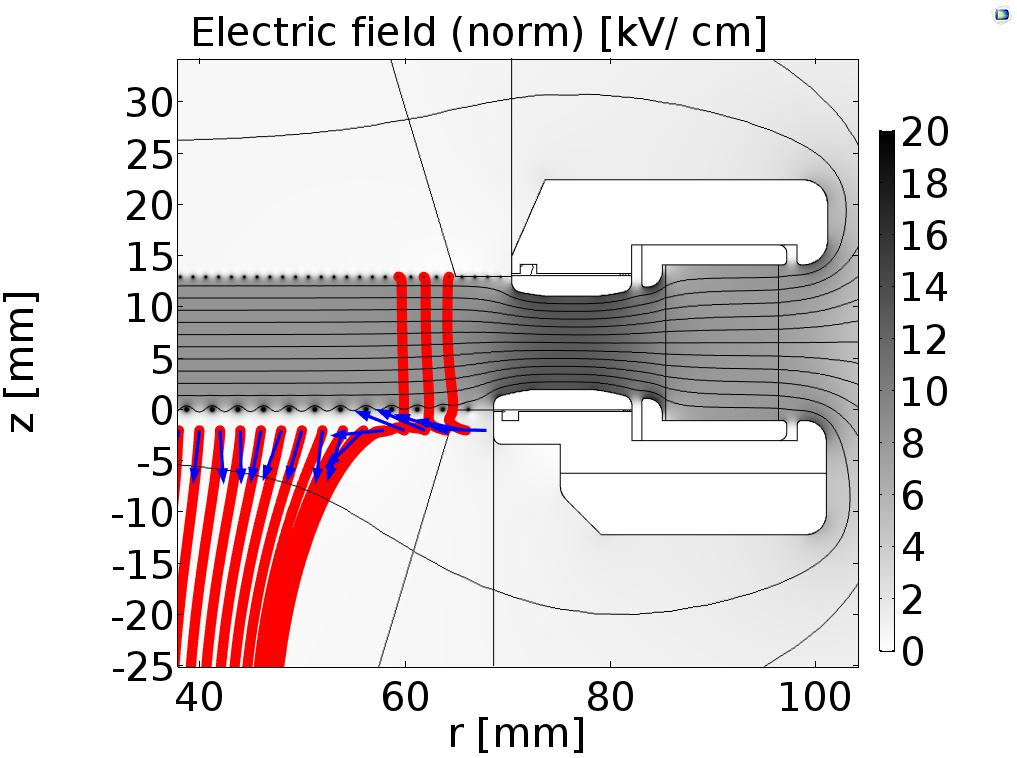
\includegraphics[width=0.8\textwidth,clip,trim={0 0 0 0},angle=0,origin=c]{Figures/GasTest/Comsol/ComsolCathodeCorner.jpg}
	\caption[Electrostatic solution of the \gtest\ detector (grid ring region).]{Electrostatic solution of the \gtest\ detector (grid ring region). This result is solved with \opvtvb\ at \SIlist{+6;-6}{kV} using COMSOL. The white metal structures in the middle of the figure are the cross sections of the grid rings. The contours show the electric potential; the color scales show the norm of electric field; the blue arrows shows the directions of the initial electron drift; the red lines shows the trajectory of electrons that start drifting at \SI{2}{\mm} below the bottom grid: electrons starting at r \SI{<60}{\mm} drift downward, when electrons starting at r \SI{>60}{\mm} drift into the EL region (cathode corner event).}
	\label{fig:gtest Comsol cathode corner}
\end{figure}

\paragraph{S1 S2 event in the EL region}
\label{sec:events particle EL region}
\label{sec:EL region event}
S1 S2 events in the EL region (EL region events) are the particle radiation events which have energy deposition location either in EL region. The process and an example waveforms is shown in Fig.~\ref{fig:EL rad event}. Since the electrons are produced in the energy deposition location in the EL region, these electrons drift in the EL region toward the anodic grid, producing EL photons. The duration of these signals are shorter compared to the \ees s because of the shorter drift length. The total quantity of photon production in this type of events is usually higher than that of an \eee , an anode cone event, and a cathode cone event, because of the free drifted electrons inside the EL region.

\begin{figure}[!htbp]
	\centering
		\begin{subfigure}[b]{.8\textwidth}
		\centering
		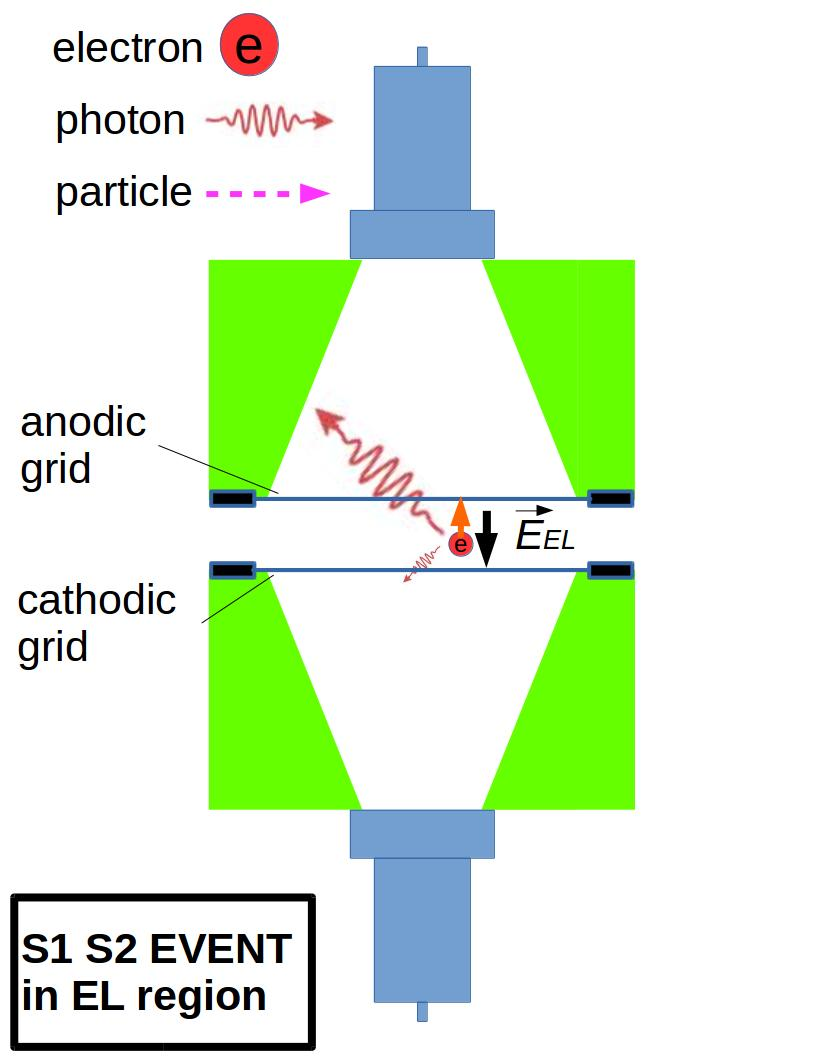
\includegraphics[width=\halfwidth,clip,trim={0 0 0 0},angle=0,origin=c]{Figures/GasTest/WeiDrawEvent/S1S2ELRegion.jpg}
		\caption{}
		\label{fig:EL rad event b}
	\end{subfigure}
	\par\bigskip
		\begin{subfigure}[b]{0.7\textwidth}
		\centering
		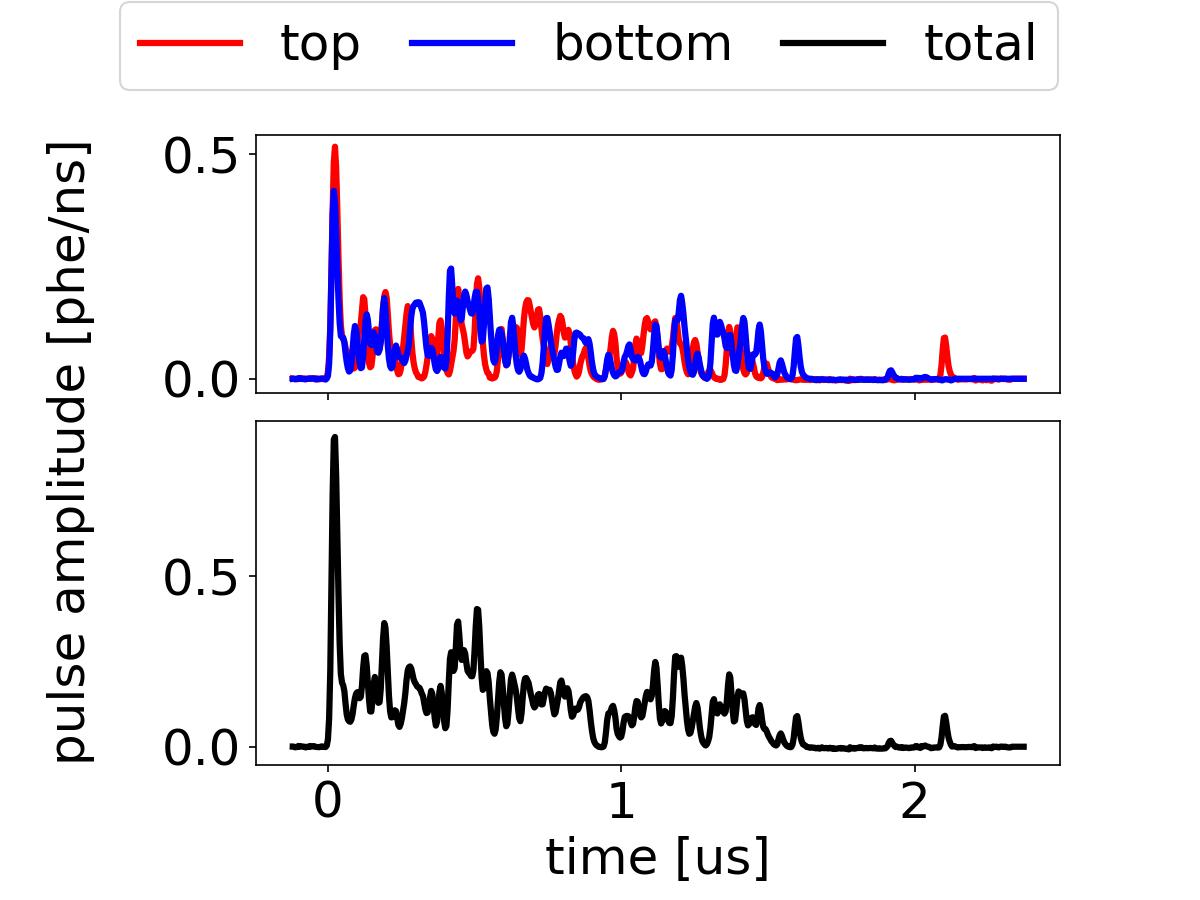
\includegraphics[width=\figurewidth,clip,trim={0 0 0 0}]{Figures/GasTest/exampleWaveforms/proc64767id00000777.jpg}
		\caption{}
		\label{fig:EL rad event a}
	\end{subfigure}
\begin{comment}
    \par\bigskip
	\begin{subfigure}[b]{0.8\textwidth}
		\centering
		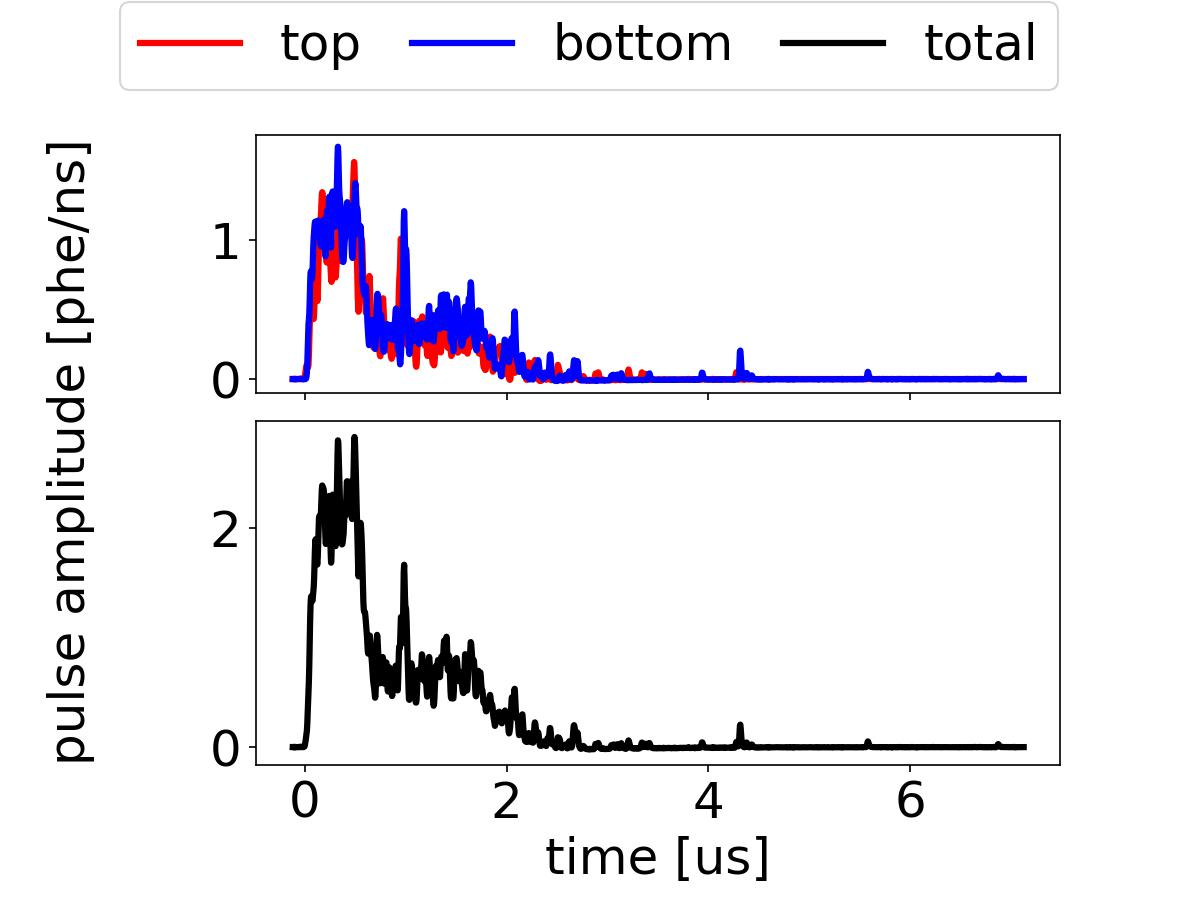
\includegraphics[width=\figurewidth,clip,trim={0 0 0 0}]{Figures/GasTest/exampleWaveforms/proc64767id00000218.jpg}%{Figures/GasTest/CutsValid/wave/testproc65831coinid0.jpg}
		\caption{}
		\label{fig:EL rad event b}
	\end{subfigure}
	\end{comment}
	\caption[\gtest\ signal: S1 S2 event in the EL region.]{\gtest\ signal: S1 S2 event in the EL region. (a) Cartoon of the process. Primary scintillation light and ionization electrons are produced from the particle interaction. The primary scintillation light and the EL light start to be produced simultaneously. (b) An example waveform of an S1 S2 event in the EL region. The primary scintillation light lies on top of the EL light. %(b) another example waveform. 
		Data were taken at \ddtt{2017}{12}{08}{14}{02}, with \opvtvb\ at \SIlist{+6;-6}{kV}, \opgd\ at \standarddensity .%Data were taken at \ddtt{2018}{03}{12}{11}{41} , with \opvtvb\ at \SI{0}{\kV}, \opgd\ at vacuum.
		% proc13001, procid:101001, Aude rename the dataset name, really confusing now.	
	}
	\label{fig:EL rad event}
\end{figure}

\paragraph{High photon count events}
High photon count events are those particle radiation events that are extremely high on energy, therefore producing plenty primary scintillation photon, free drifted electrons, and EL photons during the events. The photon production rate is so high that it exceeds the digitizing ability of the DAQ system (also called saturate the DAQ), causing distortion on waveform recording thus resulting in difficulty of signal classification. These signals may have various origins. Some of these signals have comparable or shorter duration than \ees s, two example waveforms are shown in Fig.~\ref{fig:grid wire rad} and Fig.~\ref{fig:ring rad}. These events might be related to the EL region events, described in Section~\ref{sec:EL region event}, or grid wire radiation and ring radiation, which are the particle radiation events originated from radioactive elements in grid wire and ring materials. 

%\todo{I am not confident about grid ring/wire events.}

The radioactive elements in the ring material can be both from the impurities in the material, e.g. \ce{^{238}U}, \ce{^{232}Th}, and \ce{^{235}U} and from the absorption of air on the material surfaces, e.g. \ce{^{222}Rn}. Among these sources, air radon absorption draw the most concern because of its abundance. The decay activity of radon induced radiation plating per unit of surface area per unit of time ($RA_{\text{\ce{Rn}-rad}}$) is estimated as, 
\begin{align}
	RA_{\text{\ce{Rn}-rad}} = RV_{\text{\ce{Rn}}} h_{\text{eff}} T_{\text{exposure}} \frac{1}{\tau_{\text{eff}}}
\end{align}
where $RV_{\text{\ce{Rn}}}$ is the radon decay activity in the air per unit of volume per unit of time; $h_{\text{eff}}$ is the effective height of radiation plating, in which the radon decay daughter nuclei will plate on material surface; $T_{\text{exposure}}$ is the exposure time of plating; and $\tau_{\text{eff}}$ is the effect decay time constant of radon decay daughter nuclei.
With regard to $RV_{\text{\ce{Rn}}}$ \SI{~48}{\becquerel\per\meter\cubed}, from Ref.~\cite{USEnvironmentalProtectionAgency2017}, $h_{\text{eff}}$ \SI{\sim 1}{\meter},  $\tau_{\text{eff}}$ \SI{\sim 32}{\yr}, from the decay time constant of \ce{^{210}Pb}, the typical daughter nucleus from the radon decay, in Ref.~\cite{Dulieu2008}, and $T_{\text{exposure}}$ \SI{1}{\day}, $RA_{\text{\ce{Rn}-rad}}$ is \SI{\sim 4e-3}{\becquerel\per\meter\squared}. For a \SI{\sim 40}{\cm\squared} grid wire and grid ring total surface area, The total decay activity of radon induced radiation from the ring surface is \SI{\sim e-5}{\becquerel}. These event rates should be relatively rare compared to other processes. %14 Bq total on the ring
%Dulieu2008 is LNE-CEA/LNHB reference
\begin{figure}[!htbp]
	\centering
	\begin{subfigure}[b]{.8\textwidth}
		\centering
		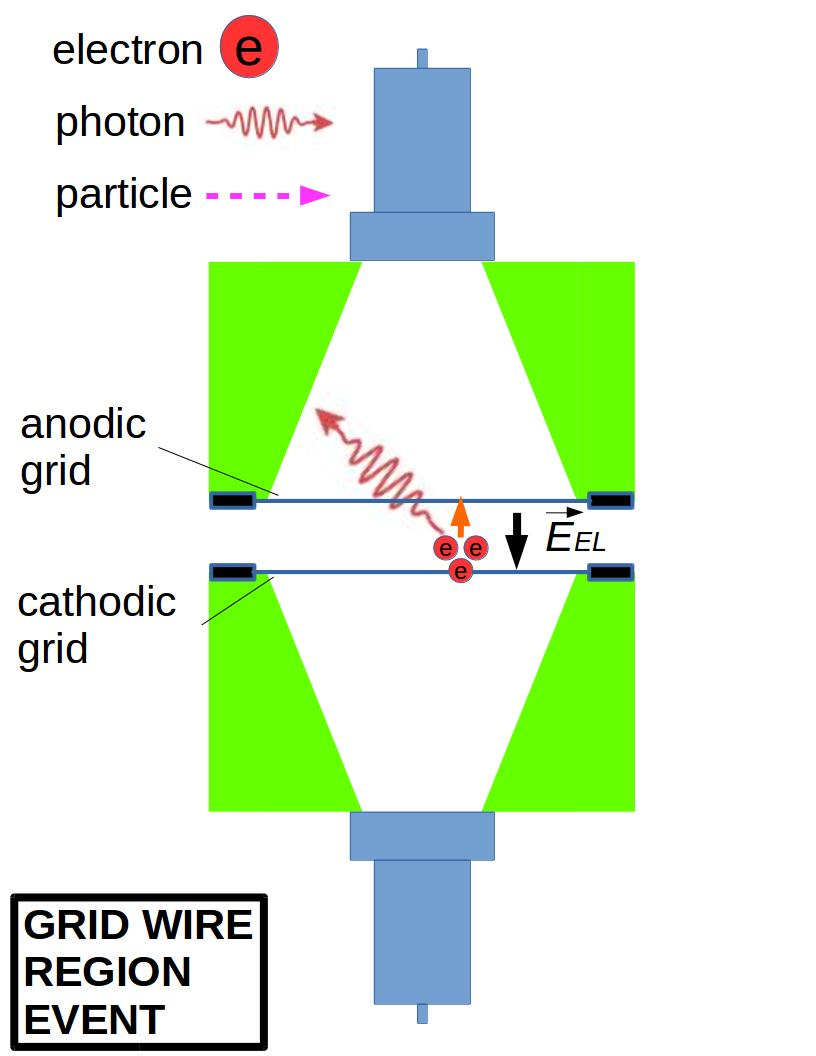
\includegraphics[width=\halfwidth,clip,trim={0 0 0 0},angle=0,origin=c]{Figures/GasTest/WeiDrawEvent/WirePhoto.jpg}
		\caption{}
		\label{fig:}
	\end{subfigure}
	\par\bigskip
	\begin{subfigure}[b]{0.7\textwidth}
		\centering
		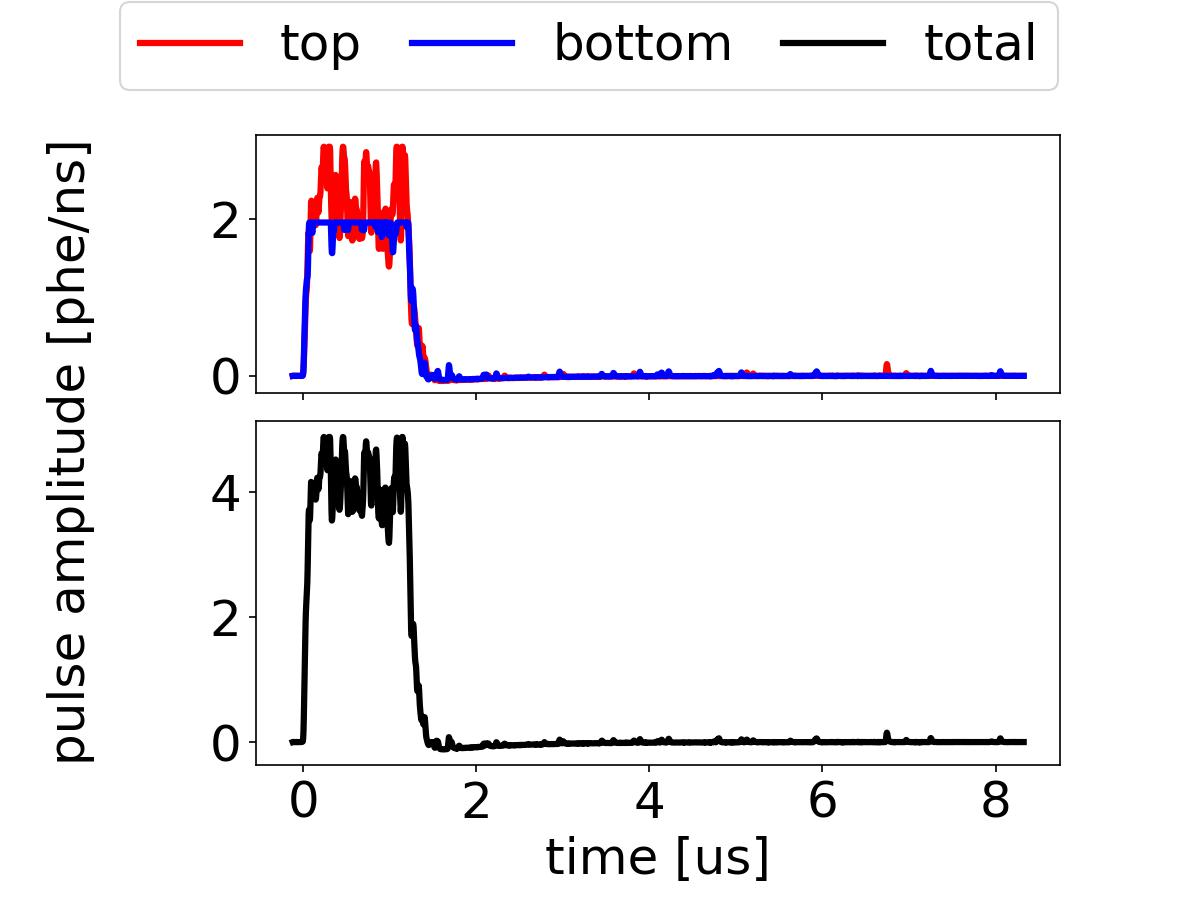
\includegraphics[width=\figurewidth,clip,trim={0 0 0 0}]{Figures/GasTest/exampleWaveforms/proc64767id00000117.jpg}%{Figures/GasTest/CutsValid/wave/testproc65831coinid0.jpg}
		\caption{}
		\label{fig:}
	\end{subfigure}
	\caption[\gtest\ signal: grid wire region event.]{\gtest\ signal: grid wire region event. (a) Cartoon of the process. (b) An example waveform. This might be an S1 S2 event in the EL region between the grid wires, when the primary scintillation light is clipped off because the signal amplitude exceeds DAQ dynamic range (PMT saturation). Data were taken at \ddtt{2017}{12}{08}{14}{02}, with \opvtvb\ at \SIlist{+6;-6}{kV}, \opgd\ at \standarddensity .%Data were taken at \ddtt{2018}{03}{12}{11}{41} , with \opvtvb\ at \SI{0}{\kV}, \opgd\ at vacuum.
		% proc13001, procid:101001, Aude rename the dataset name, really confusing now.	
	}
	\label{fig:grid wire rad}
\end{figure}
\begin{comment}
\end{comment}

\begin{figure}[!htbp]
	\centering
	\begin{subfigure}[b]{.8\textwidth}
		\centering
		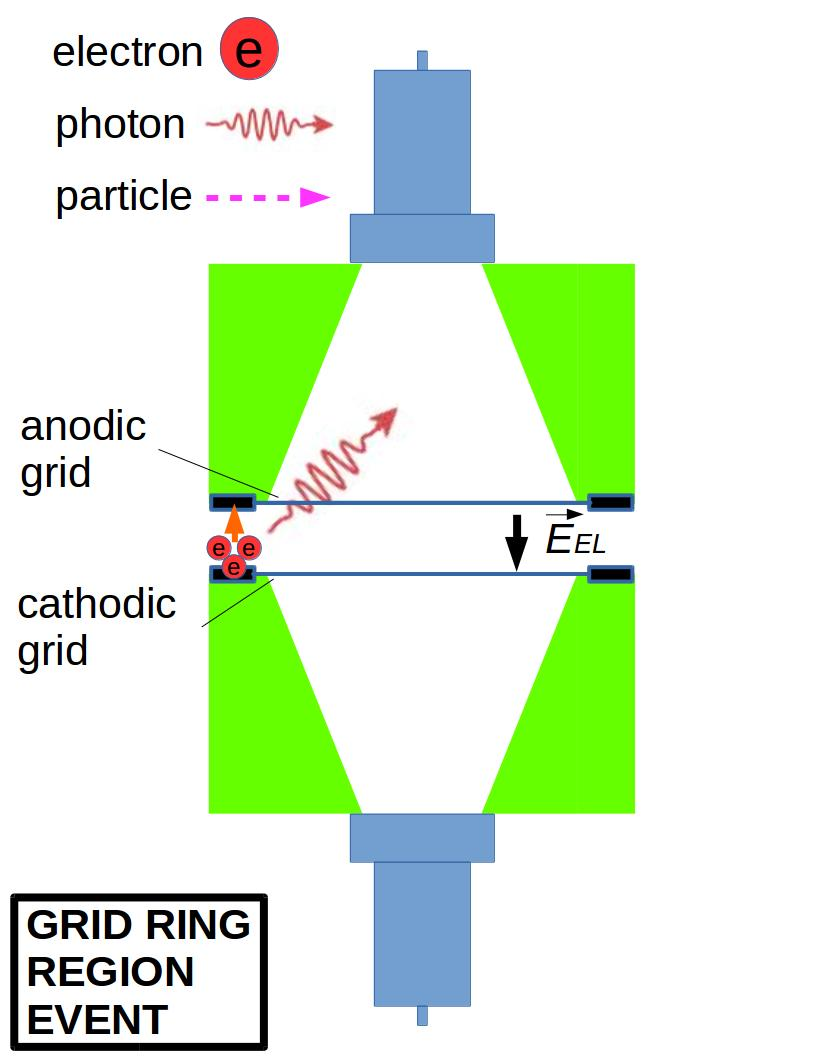
\includegraphics[width=\halfwidth,clip,trim={0 0 0 0},angle=0,origin=c]{Figures/GasTest/WeiDrawEvent/RingPhoto.jpg}
		\caption{}
		\label{fig:}
	\end{subfigure}
	\par\bigskip
	\begin{subfigure}[b]{0.7\textwidth}
		\centering
		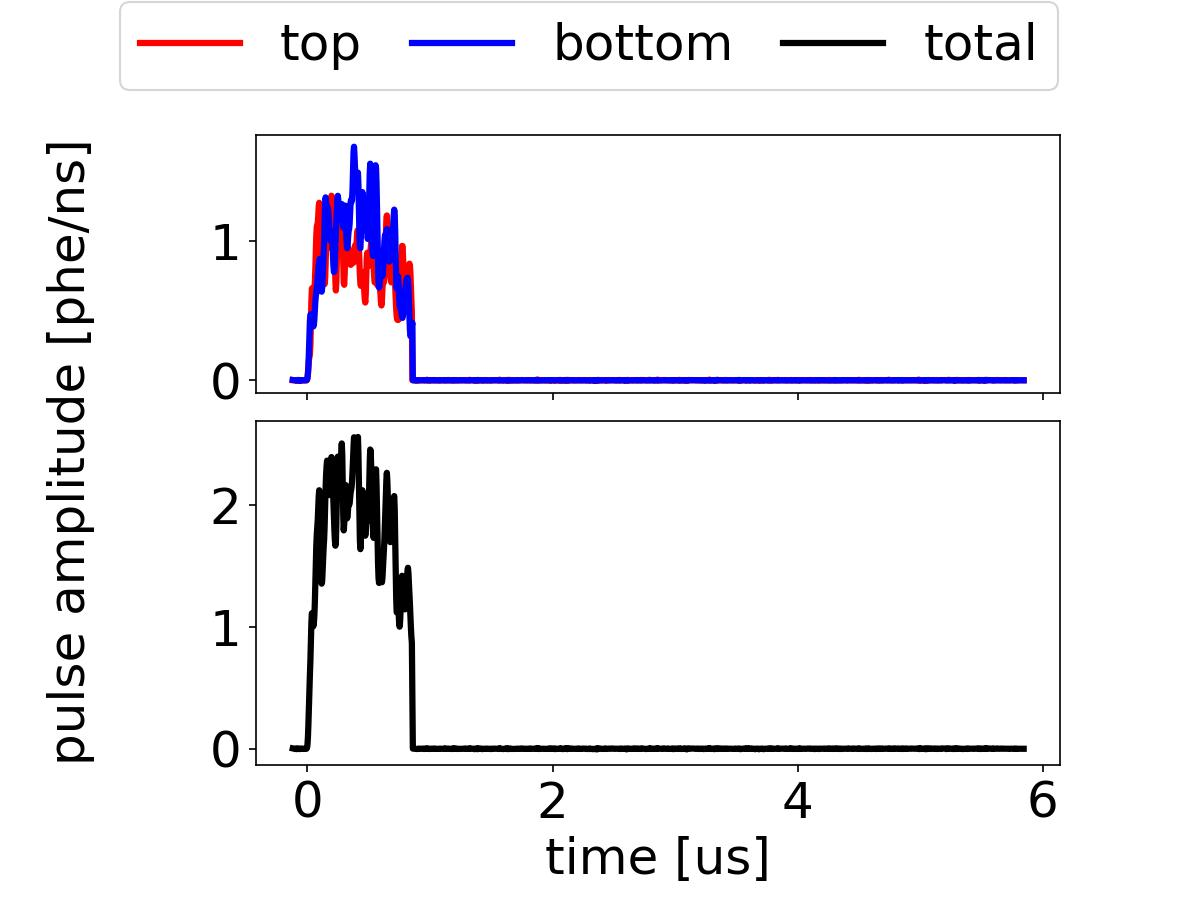
\includegraphics[width=\figurewidth,clip,trim={0 0 0 0}]{Figures/GasTest/exampleWaveforms/proc64767id00000181.jpg}
		\caption{}
		\label{fig:}
	\end{subfigure}
	\caption[\gtest\ signal: grid ring region event.]{\gtest\ signal: grid ring region event. (a) Cartoon of the process. (b) An example waveform. This might be an S1 S2 event in the EL region between the grid rings, when the primary scintillation light is not visible because the light collection efficiency is poor in this region. Data were taken at \ddtt{2017}{12}{08}{14}{02}, with \opvtvb\ at \SIlist{+6;-6}{kV}, \opgd\ at \standarddensity .%Data were taken at \ddtt{2018}{03}{12}{11}{41} , with \opvtvb\ at \SI{0}{\kV}, \opgd\ at vacuum.
		% proc13001, procid:101001, Aude rename the dataset name, really confusing now.	
	}
	\label{fig:ring rad}

\end{figure}
	\begin{comment}
\end{comment}

\paragraph{Multiple scattering events}
\label{sec:events particle multiple scatter}
Multiple scattering events are those with more than one energy deposition location. The common source of these events are a high energy gamma radiation, since it can travel far distance in the detector. The multiple scattering events usually are combinations of the previous mentioned type of events. Two example waveform are shown in Fig.~\ref{fig:multi scatter}: the first one is a multiple scattering event in the anode cone region; the second one is a multiple scattering event in the anode cone region and the EL region.

\begin{figure}[!htbp]
	\centering
	\begin{subfigure}[b]{0.7\textwidth}
		\centering
		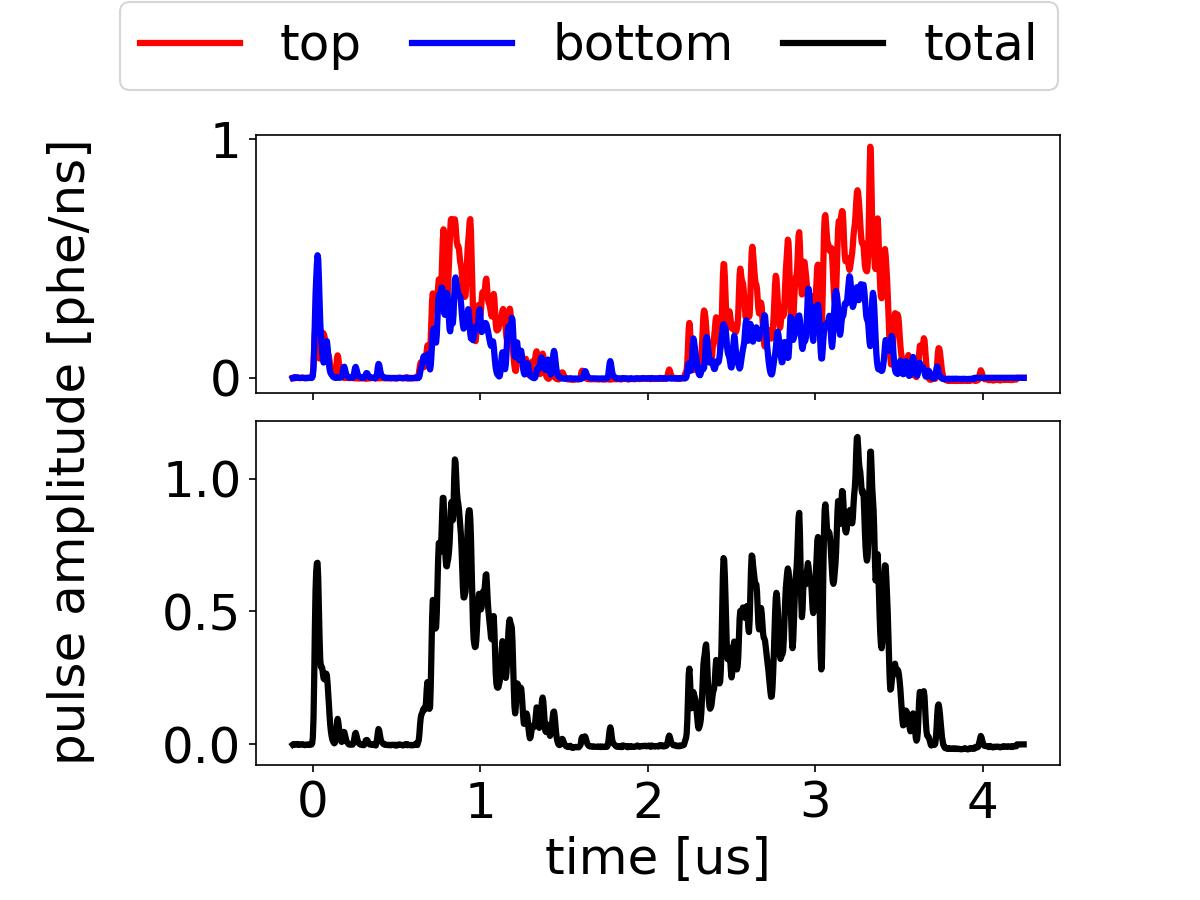
\includegraphics[width=\figurewidth,clip,trim={0 0 0 0}]{Figures/GasTest/exampleWaveforms/proc64767id00000054.jpg}
		\caption{}
		\label{fig:}
	\end{subfigure}
\par\bigskip
	\begin{subfigure}[b]{0.7\textwidth}
	\centering
	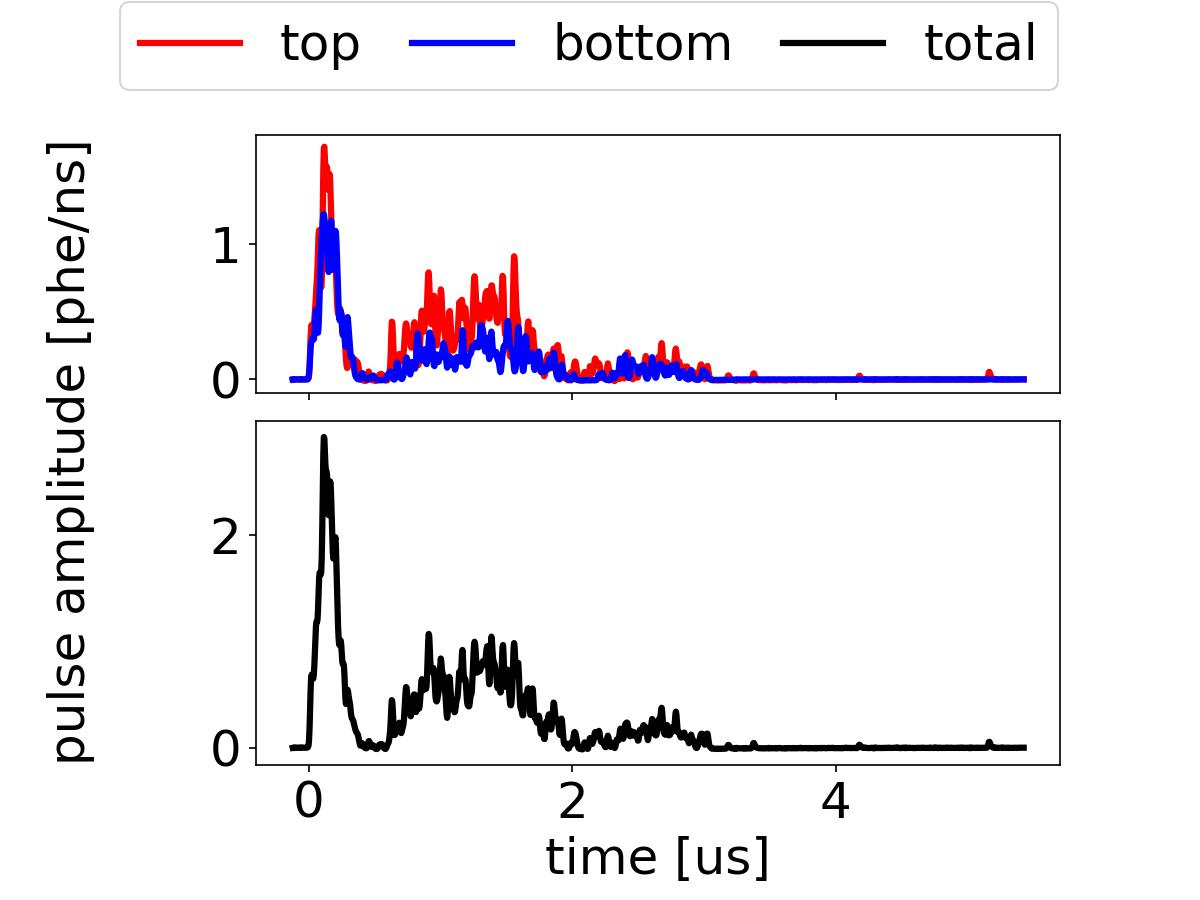
\includegraphics[width=\figurewidth,clip,trim={0 0 0 0}]{Figures/GasTest/exampleWaveforms/proc64767id00000083.jpg}
	\caption{}
	\label{fig:}
\end{subfigure}
	\caption[\gtest\ signal: multiple scattering event.]{\gtest\ signal: multiple scattering event. (a) An example waveform of a multiple scattering event in the anode cone region. (b) An example waveform of a multiple scattering event in the anode cone region and the EL region. Data were taken at \ddtt{2017}{12}{08}{14}{02}, with \opvtvb\ at \SIlist{+6;-6}{kV}, \opgd\ at \standarddensity .%Data were taken at \ddtt{2018}{03}{12}{11}{41} , with \opvtvb\ at \SI{0}{\kV}, \opgd\ at vacuum.
		% proc13001, procid:101001, Aude rename the dataset name, really confusing now.	
	}
	\label{fig:multi scatter}
\end{figure}

\subsection{Cosmic ray}
\label{sec:events muon}
Cosmic rays, originating outside Earth, are capable of producing showers of secondary particles that reach the \gtest\ detector and giving rise to signals in the detector. Among all secondary particles that raise signals, muons are the most common one because of their abundance and high penetration length in earth atmosphere. Unlike alpha, beta, and gamma particle radiation, a cosmic ray muon has a longer ionization trajectory which travels crossing the whole detector. 
%These cosmic ray muons are normally with high energy that enable them traveling in a straight line in the gas detector in less than \SI{10}{\ns}. 

The long ionization trajectory leads to a large quantity of primary scintillation light and free electron production, which results in a large light production. The minimum stop power of muon is \SI{1.255}{\MeV\per\g\cm\squared} in xenon, from Ref.~\cite{Groom2001}. In xenon gas, the reported average energy to produce a primary scintillation photon ($W_\text{sci}$) and electron-ion pair ($W_\text{ion}$) are \SI{\sim 100}{\eV} 
	\footnote{$W_\text{sci}$ is \SI[separate-uncertainty=false]{111 \pm 16}{\eV} in Ref.~\cite{Carmo2008}, and \SI[separate-uncertainty=false]{72 \pm 6}{\eV} in Ref.~\cite{Fernandes2010}.} 
	and \SI{22}{\eV} 
	\footnote{$W_\text{ion}$ is \SI{22}{\eV} in Ref.~\cite{Fano1963, Ahlen1980, Alvarez2013}.}
	, respectively. Therefore, with detector \opgd\ at \standarddensity , a muon event produce \num{\sim 2e2} primary scintillation photons and \num{\sim e3} per centimeter length of muon trajectory. The large quantity of primary scintillation light and EL light production associated with free electrons results in large signal area detected for a muon event.

Therefore, a cosmic ray muon signal has a different appearance compared to other signals because of its long ionization trajectory and large quantity of primary scintillation light and electron-ion pair production. The appearance of muon signals also varies according to their different trajectories in the detector, which will be discussed below.
%The muon events will be discussed according to their different trajectories in the detector. 
 
\paragraph{EL region muon event}
\label{sec:events muon EL region}
EL region muon events are those events that crosses the EL region, as well as the anode cone region and the cathode cone region. A cartoon and an example waveform are shown in Fig.~\ref{fig:muon EL}. Like particle radiation events, at the very beginning of the signal, primary scintillation photons are produce in the first \SI{500}{\ns}. Simultaneously, during the first \SI{2.5}{\us}, the shown signal is dominated by EL photons, which decrease in time because the electrons in the EL region land on the anodic grid thus stopping EL photon production, illustrated in Fig.~\ref{fig:muon EL b} (left). 
Since free electrons are generated all the way including the EL region, there is prompt EL light that masks the primary scintillation, causing difficulty to distinguish light from these two processes.
At a higher absolute value of \opdv , there is higher photon production per drifted electron, which results in an increase in the signal amplitude and signal area. This high signal amplitude can exceed the dynamic digitization range of the DAQ and results in a clip on the waveform, like in Fig.~\ref{fig:muon EL c}. After all electrons in the EL region reach the anodic grid, the signal is dominated by electrons originally produced in the anode cone drift to the anodic grid and EL photons are produced in the high electric field around the anodic grid, illustrated in Fig.~\ref{fig:muon EL b} (right), which is ``long tail" part of the signal in the range of \SIrange{2.5}{10}{\us} in Fig.~\ref{fig:muon EL c}.

\begin{figure}[!htbp]
	\centering
	\begin{subfigure}[b]{.8\textwidth}
		\centering
		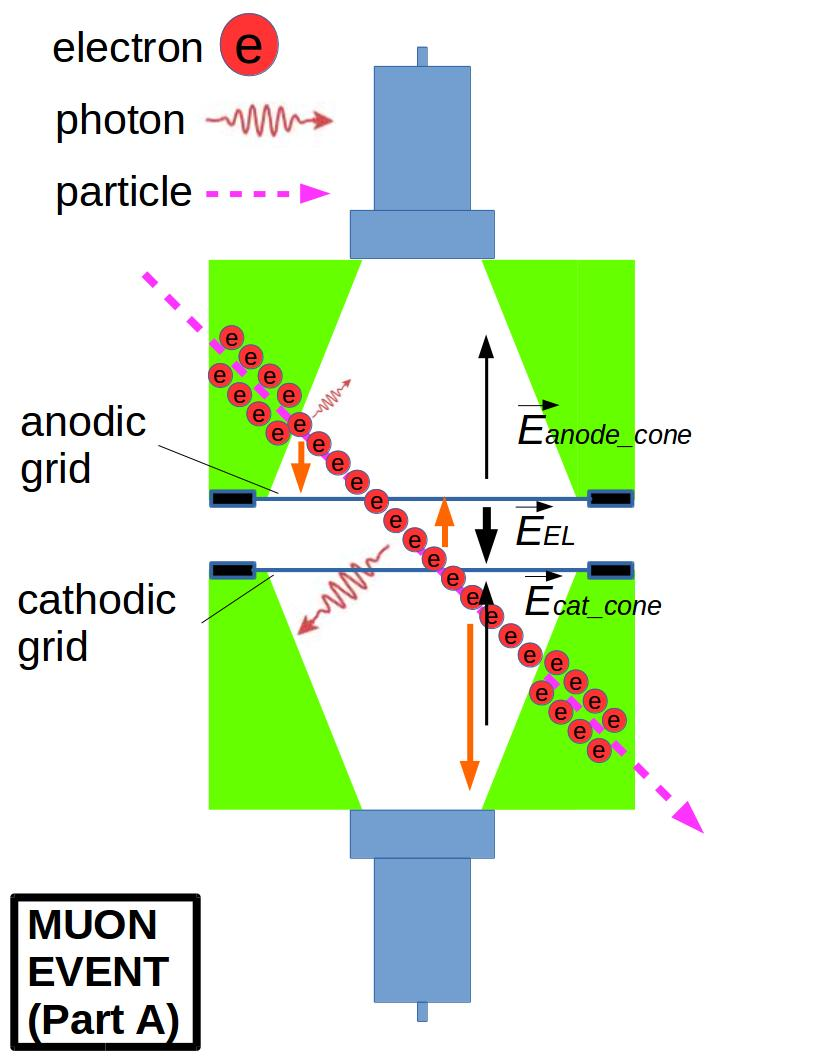
\includegraphics[width=\halfwidth,clip,trim={0 0 0 0},angle=0,origin=c]{Figures/GasTest/WeiDrawEvent/MuonEventA.jpg}
%		\caption{}
%		\label{fig:muon EL a}
%	\end{subfigure}
%	\begin{subfigure}[b]{\halfwidth}
%		\centering
		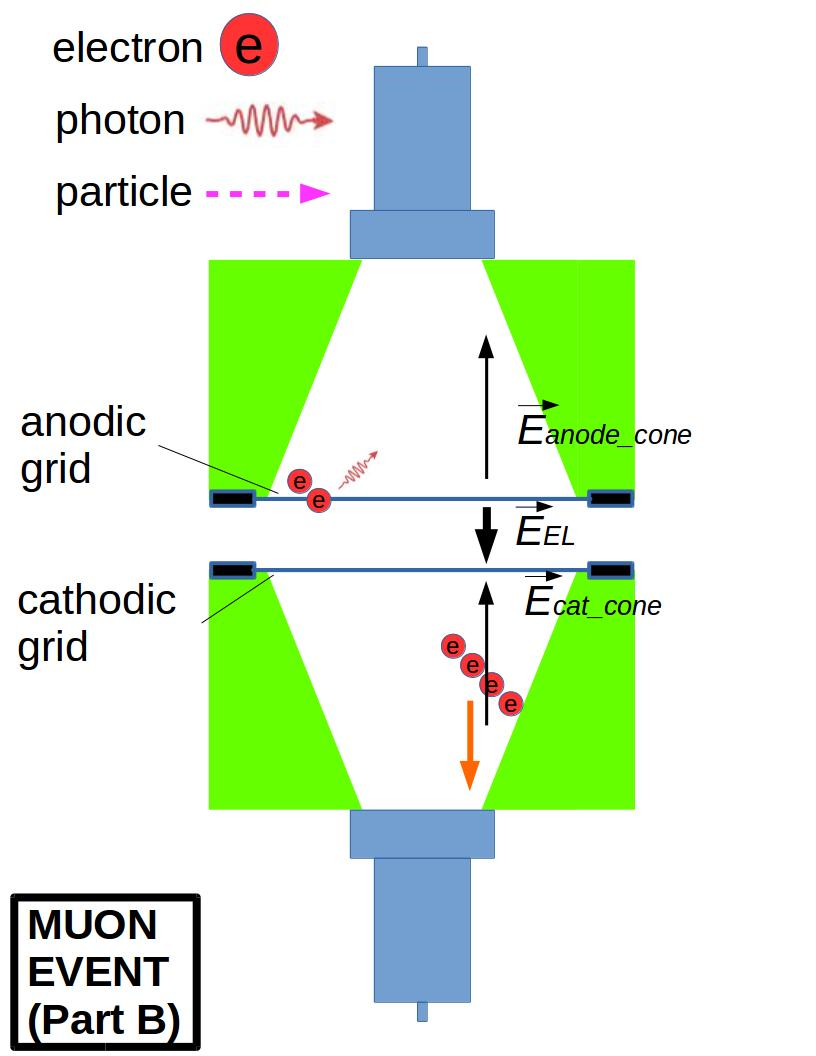
\includegraphics[width=\halfwidth,clip,trim={0 0 0 0}]{Figures/GasTest/WeiDrawEvent/MuonEventB.jpg}
		\caption{}
		\label{fig:muon EL b}
	\end{subfigure}
	\par\bigskip
	\begin{subfigure}[b]{0.6\textwidth}
		\centering
		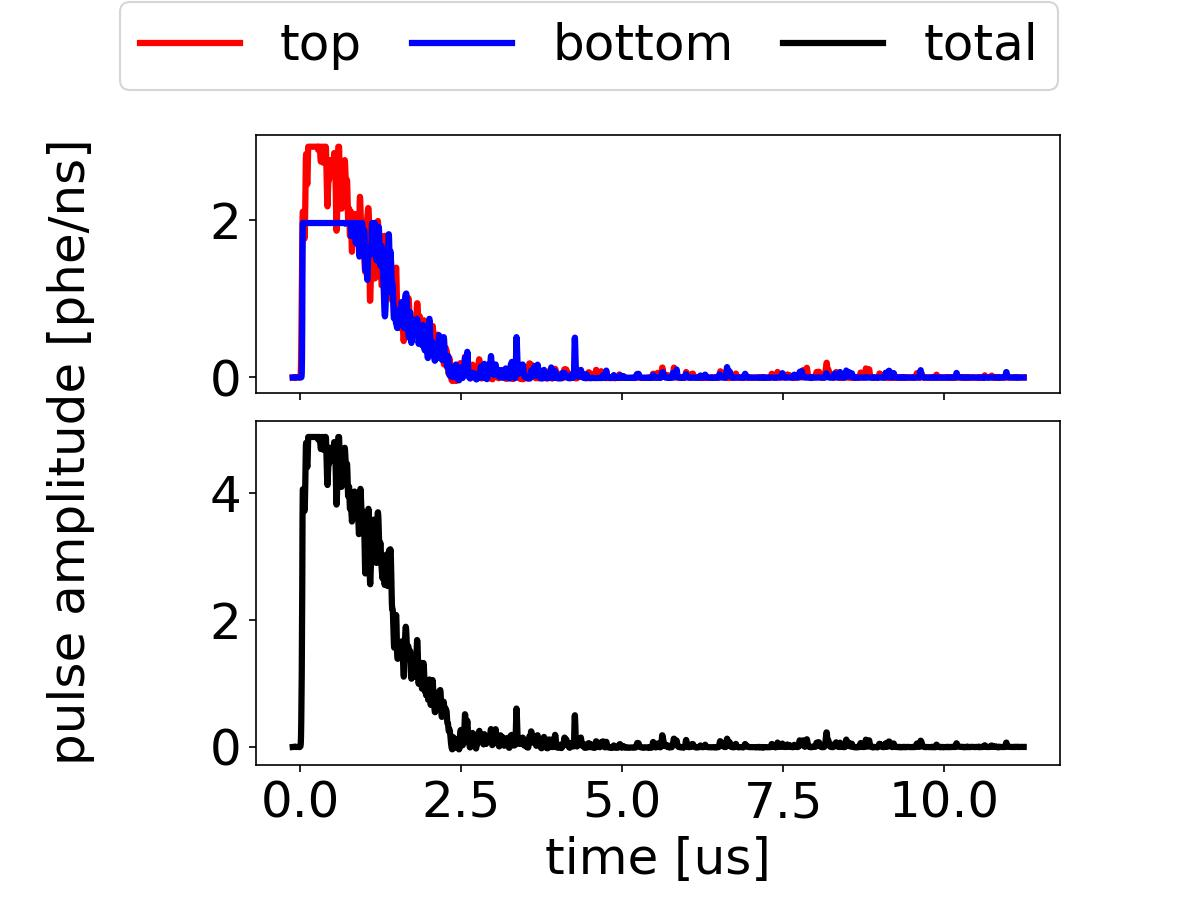
\includegraphics[width=\figurewidth,clip,trim={0 0 0 0}]{Figures/GasTest/exampleWaveforms/proc64767id00000107.jpg}
		\caption{}
		\label{fig:muon EL c}
	\end{subfigure}
\caption[\gtest\ signal: EL region muon event.]{\gtest\ signal: EL region muon event. (a) Cartoon of the process. Left: Primary scintillation light and ionization electrons are produced along the muon trajectory, and ionization electrons drift according to the direction of the electric field. EL light also start to be produced by the ionization electrons in the EL region (part A). Right: EL light is produced in the high electric field region around the anodic grid wires (part B). (b) An example waveform of an EL region muon event. The right-angled triangle shape waveform before \SI{2.5}{\us} is the EL light produced in the EL region (cartoon part A). The primary scintillation light is clipped off because of the PMT saturation. The ``long tail" after \SI{2.5}{\us} is the EL light produced around the anodic grid wires (cartoon part B). Data were taken at \ddtt{2017}{12}{08}{14}{02}, with \opvtvb\ at \SIlist{+6;-6}{kV}, \opgd\ at \standarddensity .} 
	\label{fig:muon EL}
\end{figure}

EL region muon events between grid rings are those events that crosses the EL region between the grid rings, without crossing the anode cone region. The cartoon of this process is shown in Fig.~\ref{fig:muon ring a}. Similar to other EL region muon events, these events produces primary scintillation light and EL light between the grid rings. However, since the muon trajectory does not cross the anode cone region, there are no free electrons produced in such region, which leads to the absence of the ``long tail" in the signal, as shown in Fig.~\ref{fig:muon ring b}.  

\begin{figure}[!htbp]
	\centering
	\begin{subfigure}[b]{.8\textwidth}
		\centering
		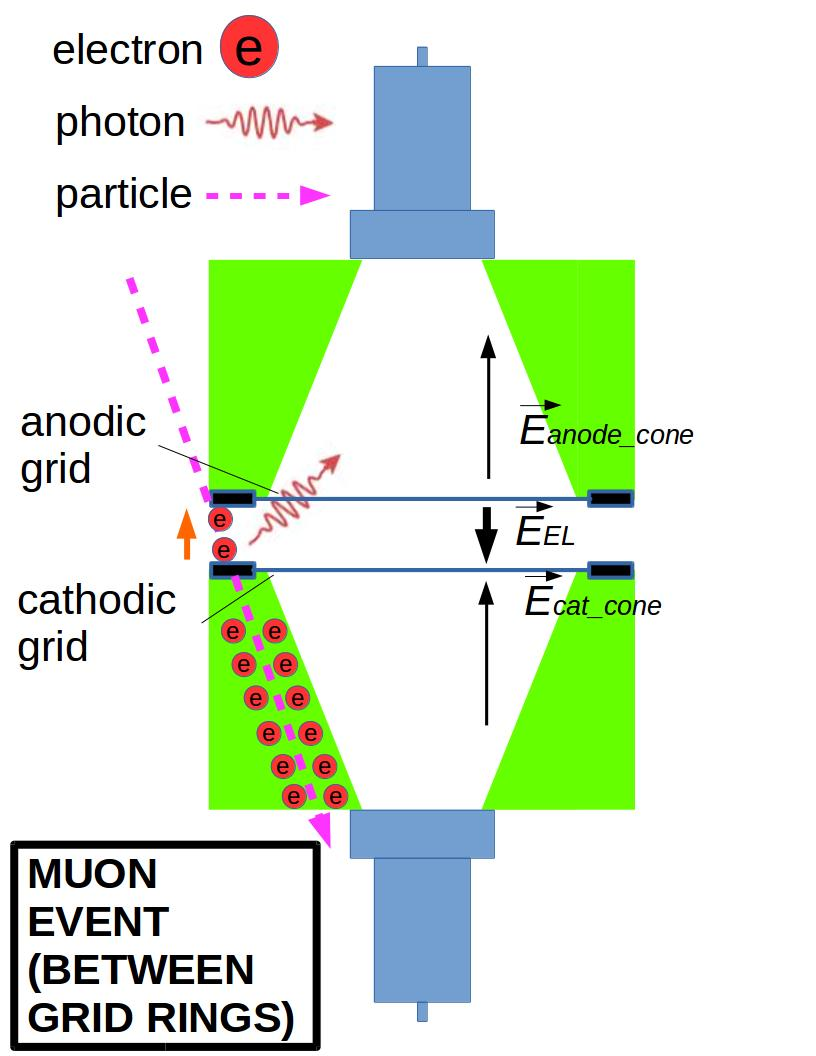
\includegraphics[width=\halfwidth,clip,trim={0 0 0 0},angle=0,origin=c]{Figures/GasTest/WeiDrawEvent/MuonEventRing.jpg}
		\caption{}
		\label{fig:muon ring a}
	\end{subfigure}
	\par\bigskip
	\begin{subfigure}[b]{0.7\textwidth}
		\centering
		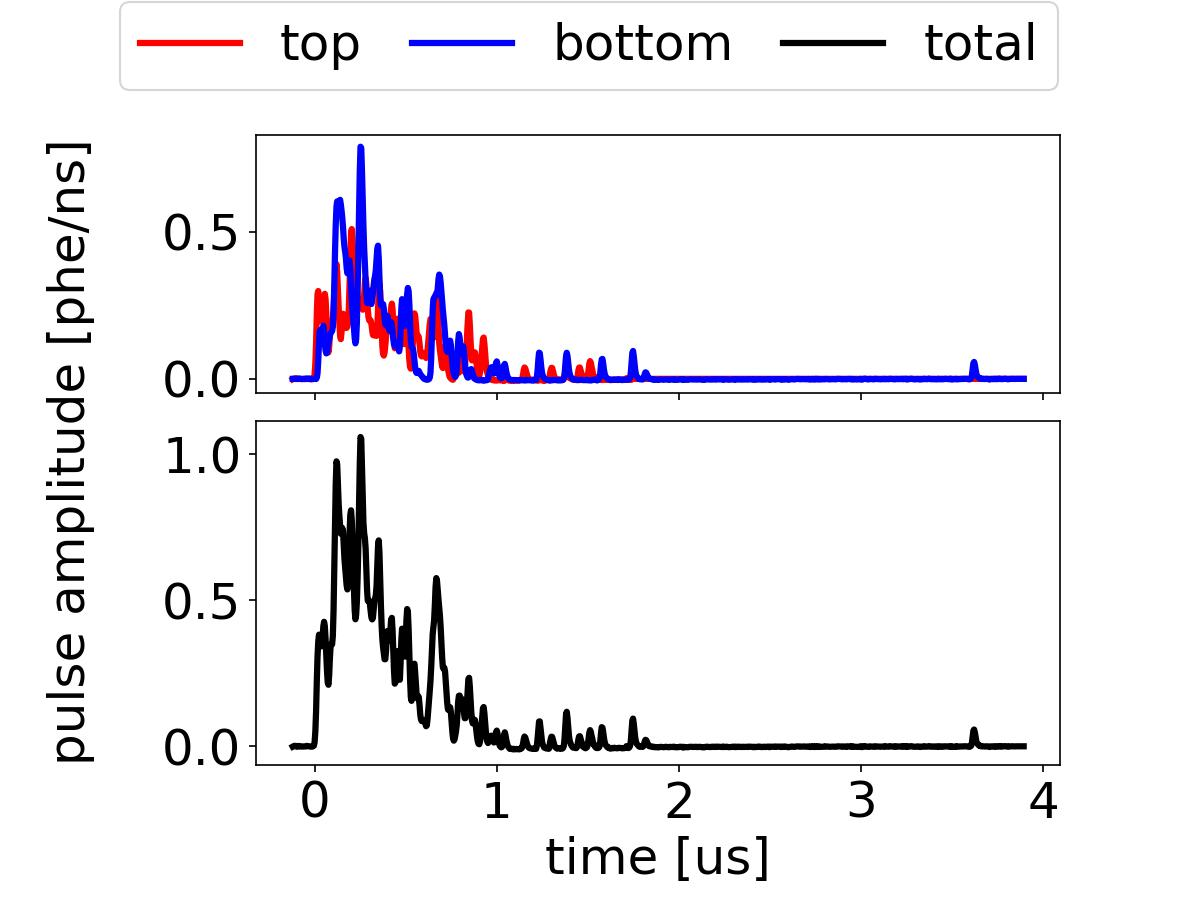
\includegraphics[width=\figurewidth,clip,trim={0 0 0 0}]{Figures/GasTest/exampleWaveforms/proc64767id00000003.jpg}%{Figures/GasTest/CutsValid/wave/testproc65831coinid0.jpg}
		\caption{}
		\label{fig:muon ring b}
	\end{subfigure}
	\caption[\gtest\ signal: muon event between the grid rings.]{\gtest\ signal: muon event between the grid rings. (a) Cartoon of the process. This process is similar to that of the EL region muon event except there are no electrons produced in the anode cone region. (b) An example waveform. The absence of ``long tail"  is because of the absence of electrons produced in the anode cone region. Data were taken at \ddtt{2017}{12}{08}{14}{02}, with \opvtvb\ at \SIlist{+6;-6}{kV}, \opgd\ at \standarddensity .%Data were taken at \ddtt{2018}{03}{12}{11}{41} , with \opvtvb\ at \SI{0}{\kV}, \opgd\ at vacuum.
		% proc13001, procid:101001, Aude rename the dataset name, really confusing now.	
	}
	\label{fig:muon ring}
\end{figure}

\paragraph{Anode cone muon event}
\label{sec:events muon anode cone}
Anode cone muon events are those events that crosses only the anode cone region. A cartoon and an example waveform are shown in Fig.~\ref{fig:muon anode}. At the very beginning of the signal, primary scintillation photons are produce in the first \SI{500}{\ns}, the process and waveform of which are shown in Fig.~\ref{fig:muon anode a} and Fig.~\ref{fig:muon anode d}. Next, electrons originally produced in the anode cone drift to the anodic grid and EL photons are produced in the high electric field around the anodic grid, the process and waveform of which are shown in Fig.~\ref{fig:muon anode b} and Fig.~\ref{fig:muon anode e}. 

\begin{figure}[!htbp]
	\centering
	\begin{subfigure}[b]{0.8\textwidth}
		\centering
		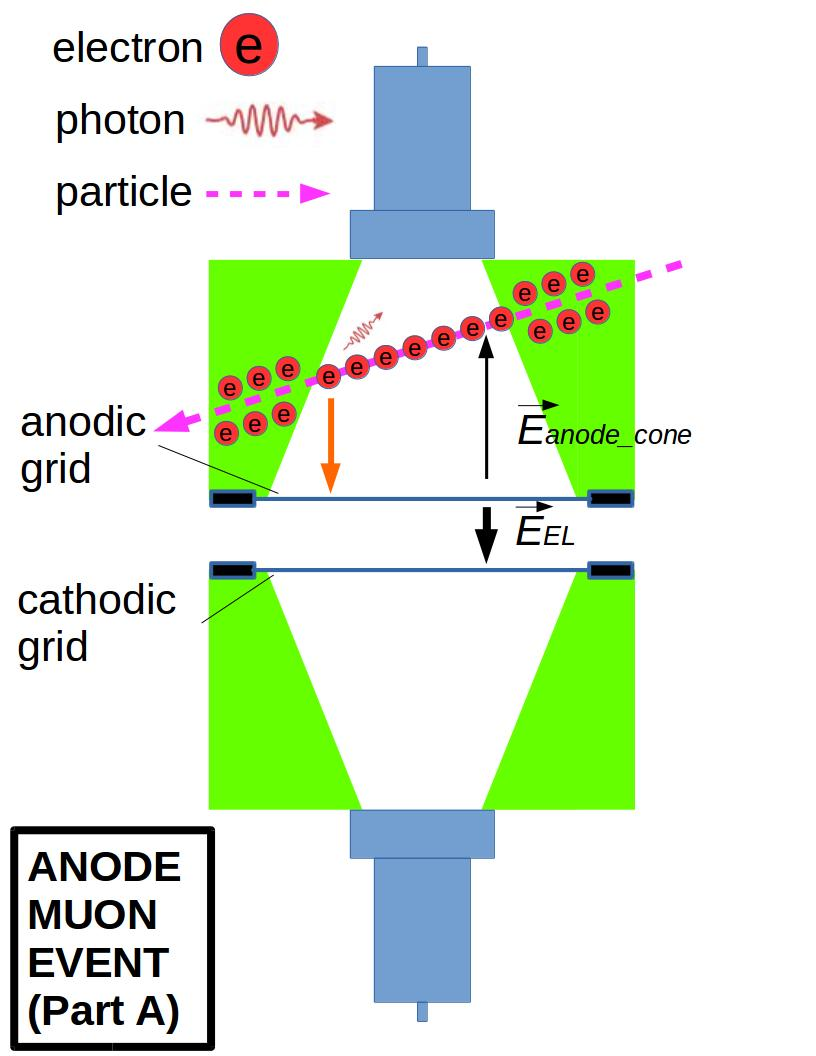
\includegraphics[width=\halfwidth,clip,trim={0 0 0 0},angle=0,origin=c]{Figures/GasTest/WeiDrawEvent/AnodeMuonEventA.jpg}
%		\caption{}
%		\label{fig:muon anode a}
%	\end{subfigure}
%	\begin{subfigure}[b]{\halfwidth}
%		\centering
		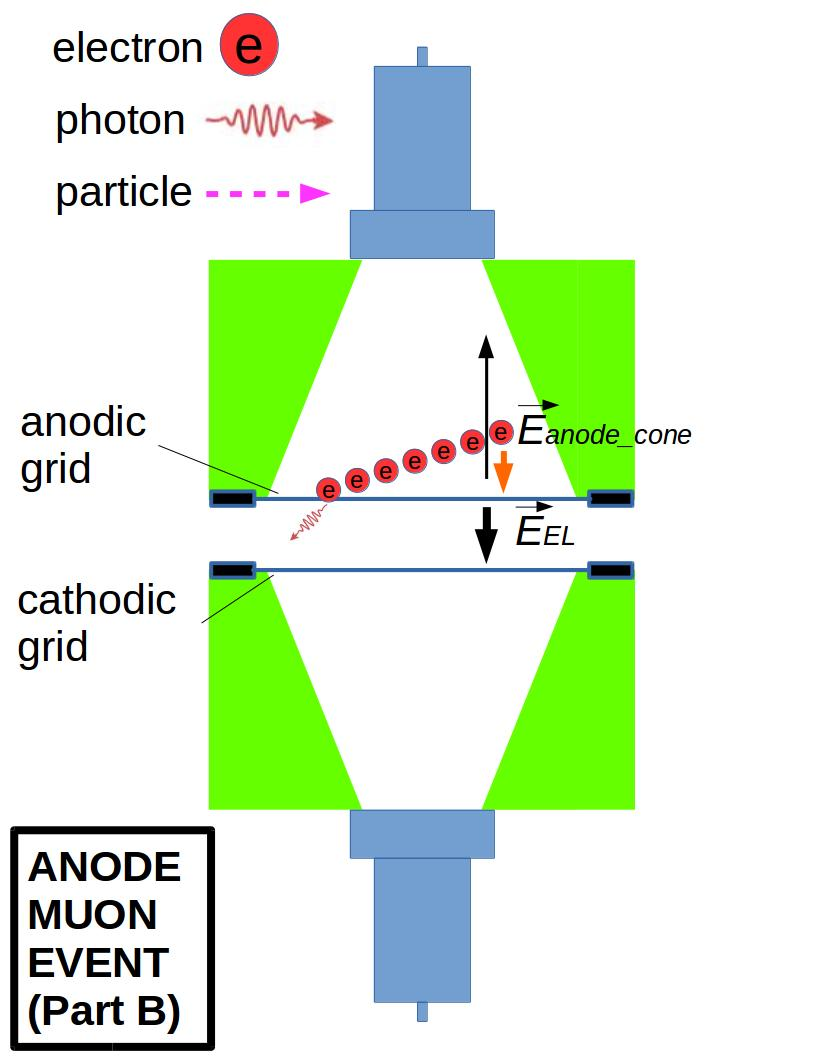
\includegraphics[width=\halfwidth,clip,trim={0 0 0 0}]{Figures/GasTest/WeiDrawEvent/AnodeMuonEventB.jpg}
		\caption{}
		\label{fig:muon anode b}
	\end{subfigure}
	\par\bigskip
	\begin{subfigure}[b]{0.7\textwidth}
		\centering
		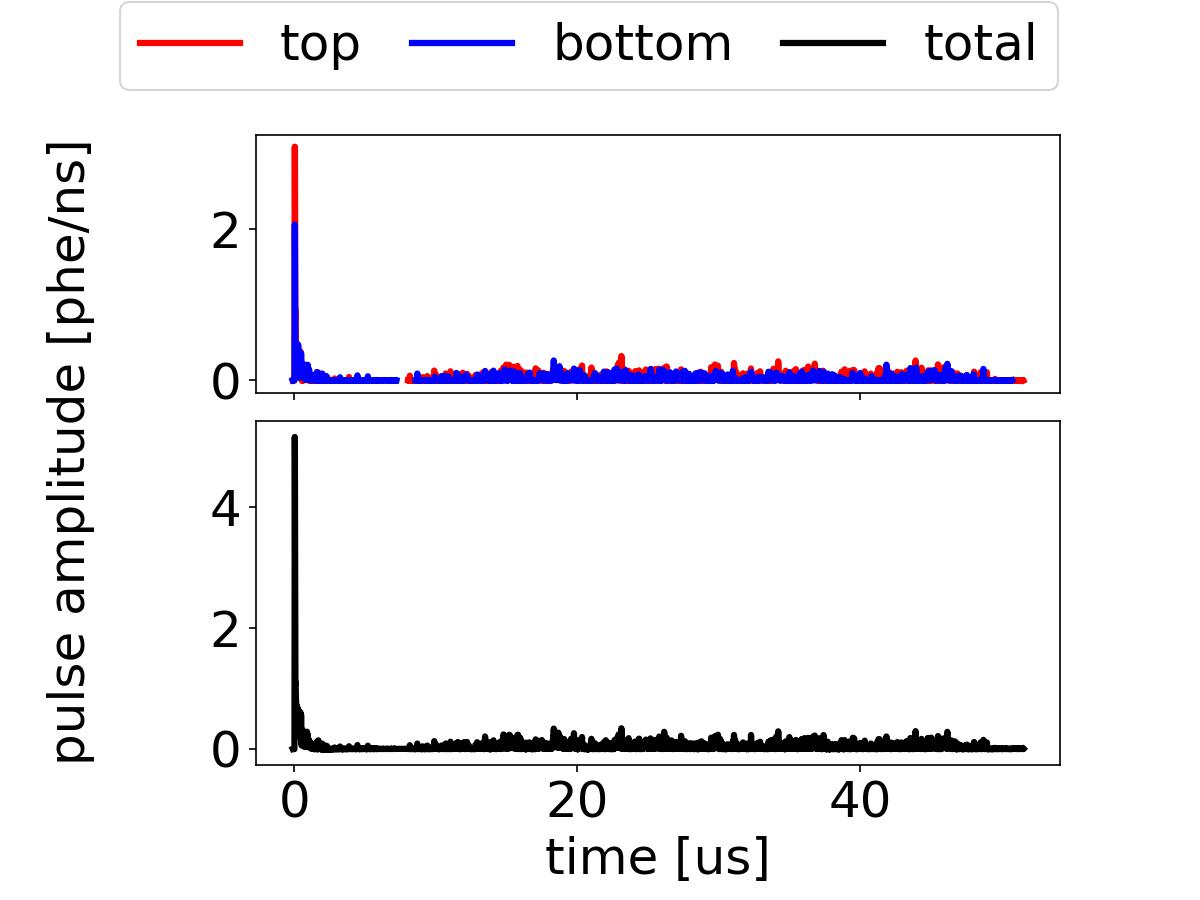
\includegraphics[width=\figurewidth,clip,trim={0 0 0 0}]{Figures/GasTest/exampleWaveforms/proc64767AnodeMuon1.jpg}
		\caption{}
		\label{fig:muon anode c}
	\end{subfigure}
	\caption[\gtest\ signal: anode cone muon event.]{\gtest\ signal: anode cone muon event. (a) Cartoon of the process. This process is similar to that of the EL region muon event except for there are no electrons produced in the EL region. (b) An example waveform of an anode muon cone event. The absence of the ``right-angled triangle shape waveform"  is because of the absence of electrons produced in the EL region. Data were taken at \ddtt{2017}{12}{08}{14}{02}, with \opvtvb\ at \SIlist{+6;-6}{kV}, \opgd\ at \standarddensity .}
	\label{fig:muon anode}
\end{figure}
\begin{figure}[!htbp]\ContinuedFloat
	\centering
	\begin{subfigure}[b]{0.7\textwidth}
		\centering
		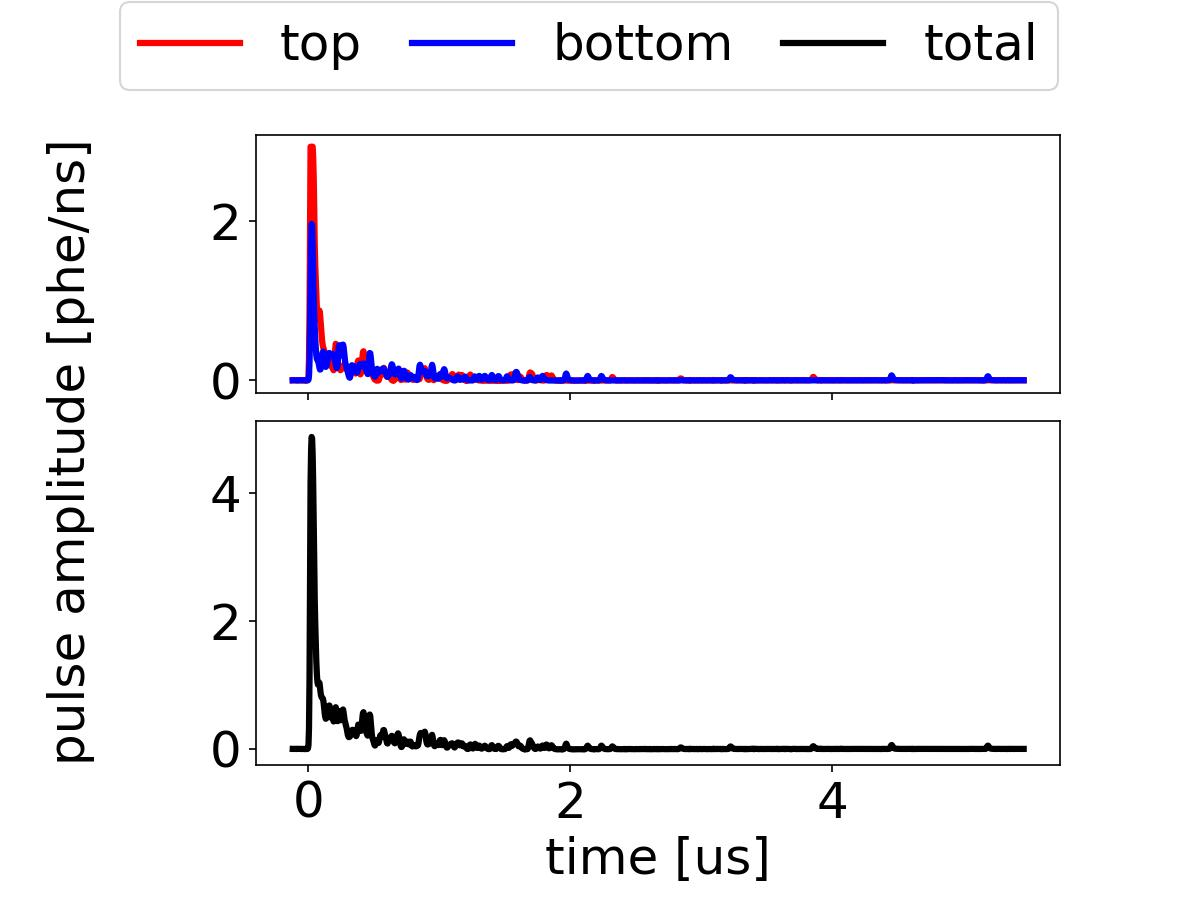
\includegraphics[width=\figurewidth,clip,trim={0 0 0 0}]{Figures/GasTest/exampleWaveforms/proc64767AnodeMuon1P1.jpg}
		\caption{}
		\label{fig:muon anode d}
	\end{subfigure}
		\par\bigskip
\begin{subfigure}[b]{0.7\textwidth}
	\centering
	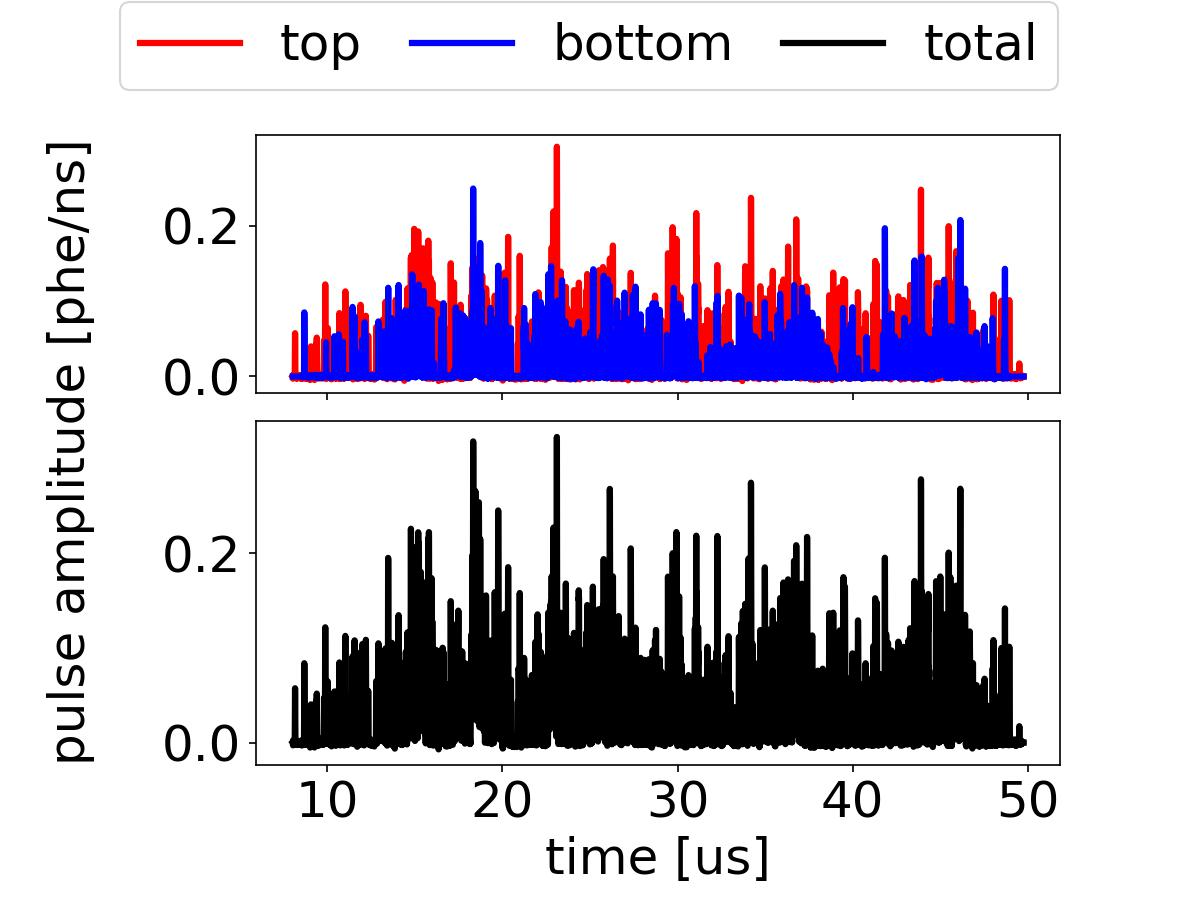
\includegraphics[width=\figurewidth,clip,trim={0 0 0 0}]{Figures/GasTest/exampleWaveforms/proc64767AnodeMuon1P2.jpg}
	\caption{}
	\label{fig:muon anode e}
\end{subfigure}
	\caption[\gtest\ signal: anode cone muon event (cont.).]{\gtest\ signal: anode muon cone event (cont.). (c) An example waveform of an anode muon cone event, zoomed in the range of \SIrange{0}{5}{\us}, which shows the primary scintillation light (cartoon part A). (d) An example waveform of an anode cone muon event, zoomed in the range of \SIrange{6}{50}{\us}, which shows the EL light produced around the anodic grid wires (cartoon part B).}
	\label{fig:anode muon cont}
\end{figure}

\paragraph{Cathode cone muon event}
\label{sec:events muon cathode cone}
Cathode cone muon events are those events that crosses only the cathode cone region. A cartoon and an example waveform are shown in Fig.~\ref{fig:cathode muon}. At the very beginning of the signal, primary scintillation photons are produce in the first \SI{500}{\ns}, the process and waveform of which are shown in Fig.~\ref{fig:cathode muon a} and Fig.~\ref{fig:cathode muon b}. Next, electrons originally produced in the cathode cone drift to the cathode PMT associated with few EL photons production in this low electric field cathode cone region. 

\begin{figure}[!htbp]
	\centering
		\begin{subfigure}[b]{.8\textwidth}
		\centering
		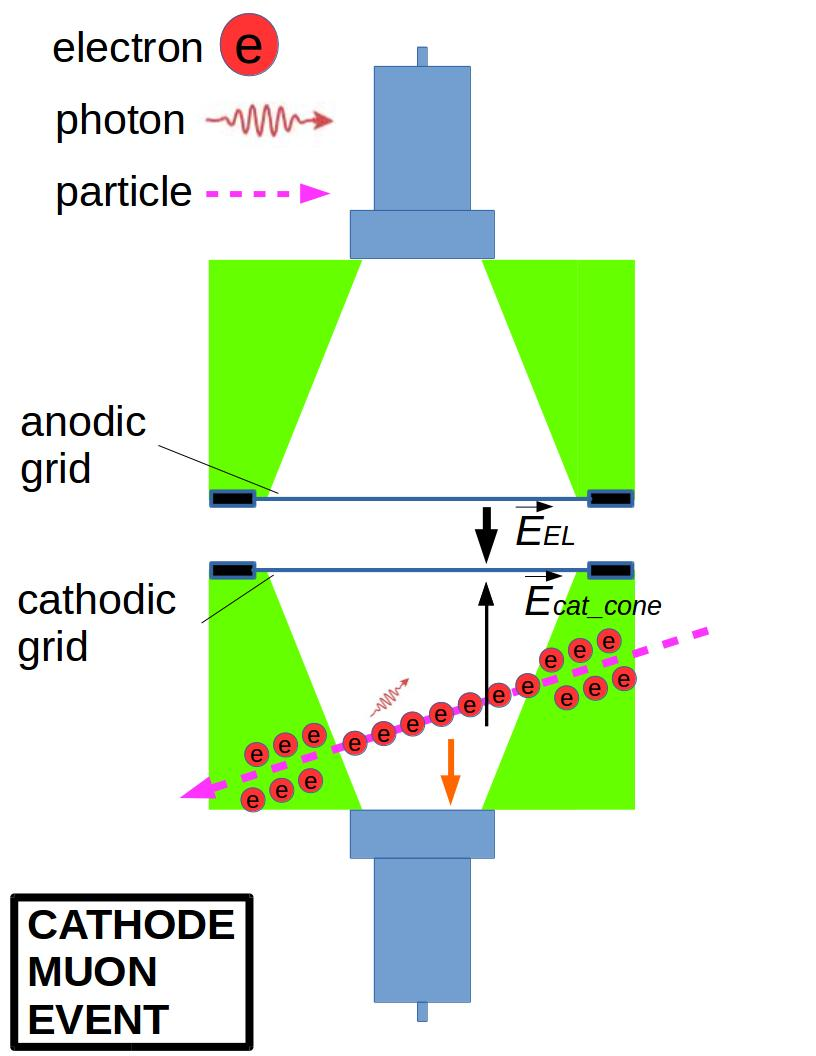
\includegraphics[width=\halfwidth,clip,trim={0 0 0 0},angle=0,origin=c]{Figures/GasTest/WeiDrawEvent/CathodeMuonEvent.jpg}
		\caption{}
		\label{fig:cathode muon a}
	\end{subfigure}
\par\bigskip
	\begin{subfigure}[b]{0.7\textwidth}
		\centering
		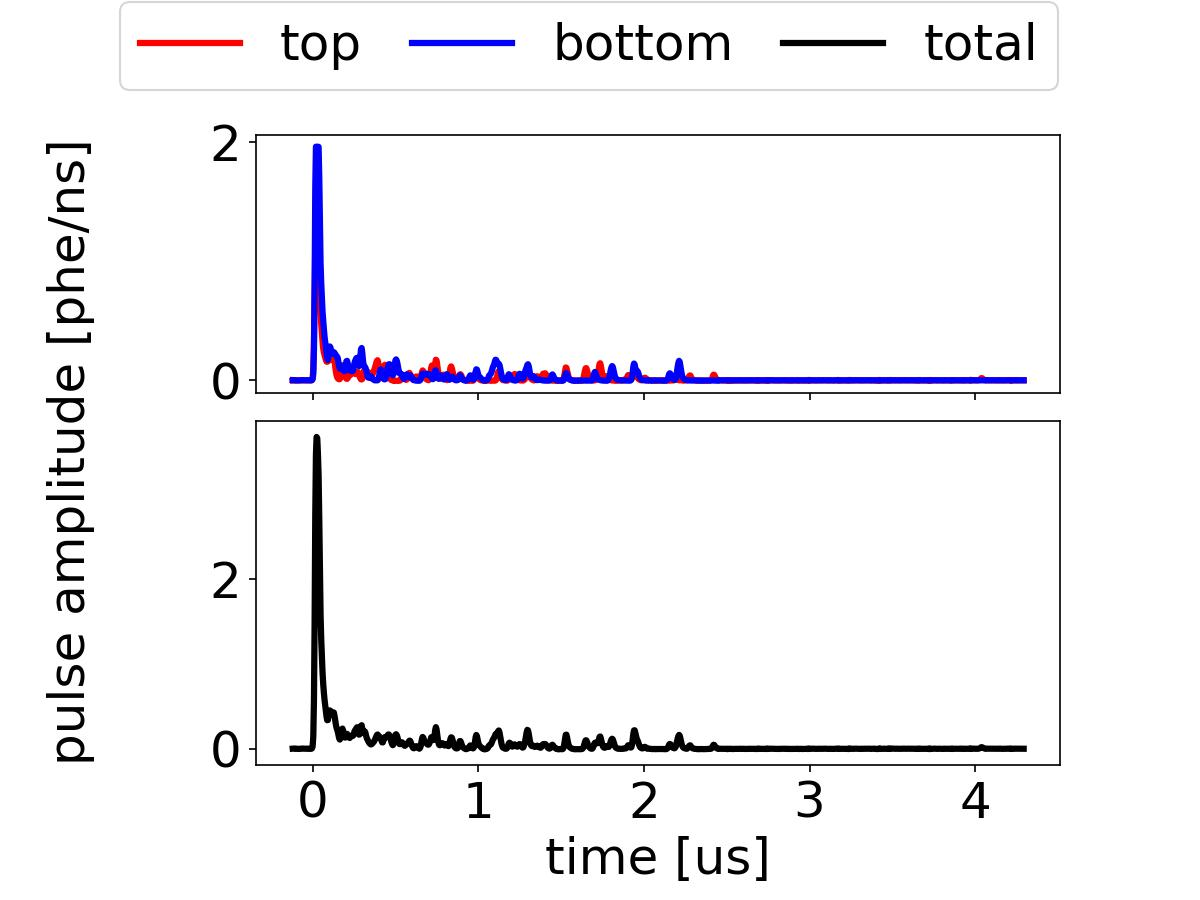
\includegraphics[width=\figurewidth,clip,trim={0 0 0 0}]{Figures/GasTest/exampleWaveforms/proc64767id00000007.jpg}%{Figures/GasTest/CutsValid/wave/testproc65831coinid0.jpg}
		\caption{}
		\label{fig:cathode muon b}
	\end{subfigure}
	\caption[\gtest\ signal: cathode cone muon event.]{\gtest\ signal: cathode cone muon event. (a) Cartoon of the process. This process is similar to that of the EL region muon event except for there are no electrons produced in the EL region or the anode cone region. (b) An example waveform of a cathode muon cone event. The absence of the ``right-angled triangle shape waveform" and the ``long tail"  is because of the absence of electrons produced in the EL region and the anode cone region.  Data were taken at \ddtt{2017}{12}{08}{14}{02}, with \opvtvb\ at \SIlist{+6;-6}{kV}, \opgd\ at \standarddensity .%Data were taken at \ddtt{2018}{03}{12}{11}{41} , with \opvtvb\ at \SI{0}{\kV}, \opgd\ at vacuum.
		% proc13001, procid:101001, Aude rename the dataset name, really confusing now.	
	}
	\label{fig:cathode muon}
\end{figure}

\subsection{Other miscellaneous sources}
\label{sec:events misc}
\paragraph{Electrical noise} 
\label{sec:events noise}
Electrical noise are the disturbance in an electrical system during signal transfer. Electrical noise can come from both internal and external sources to the system, and can add to the systematic fluctuation of other signals from the \gtest detector. This systematic fluctuation is characterized by the baseline fluctuation, whose amplitude is \SI{\sim 0.36}{\mV}, which is very small compared to signal amplitude of the wanted signals. 

Electrical noise from the external electrical grounding of the infrastructures and the KNF pump, however, has an amplitude up to \SI{5}{\mV} and is capable of start a separate pulse recording sometimes; this type of electrical noise is called electrical noise signals. An example waveform of electrical noise signal is shown in Fig.~\ref{fig:noise}. As shown in this figure, an electrical noise signal is likely to have the waveforms in both PMTs overlapping. %a comparable signal negative maximum amplitude and signal positive amplitude, and a small and sometimes negative signal total pulse area. 
The waveform in each PMT is bipolar and symmetric; that is, the positive and negative maxima of the waveform amplitude are about the same. The bipolar and symmetric aspect of the waveform leads to a near-zero integral of the signal area, which don't give a meaningful waveform shape RQs because these RQ algorithms are designed for a unipolar signal. 
%The negative total pulse area usually also makes it impossible to find the pulse RQs of characteristic waveform percentiles to conduct further signal \ees\ selections. 
Therefore, to reduce the influence of these electrical noise signals, the KNF pump is turn off during all measurements and we improved on the electrical grounding of infrastructure. After this improvement, electrical noise signals occur at a rate of \SI{\sim 2}{\Hz}, which are further addressed by signal selections based on the bipolar feature of the noise signals. 

\begin{figure}[!p]
    \centering
	\begin{subfigure}[b]{0.7\textwidth}
	\centering
	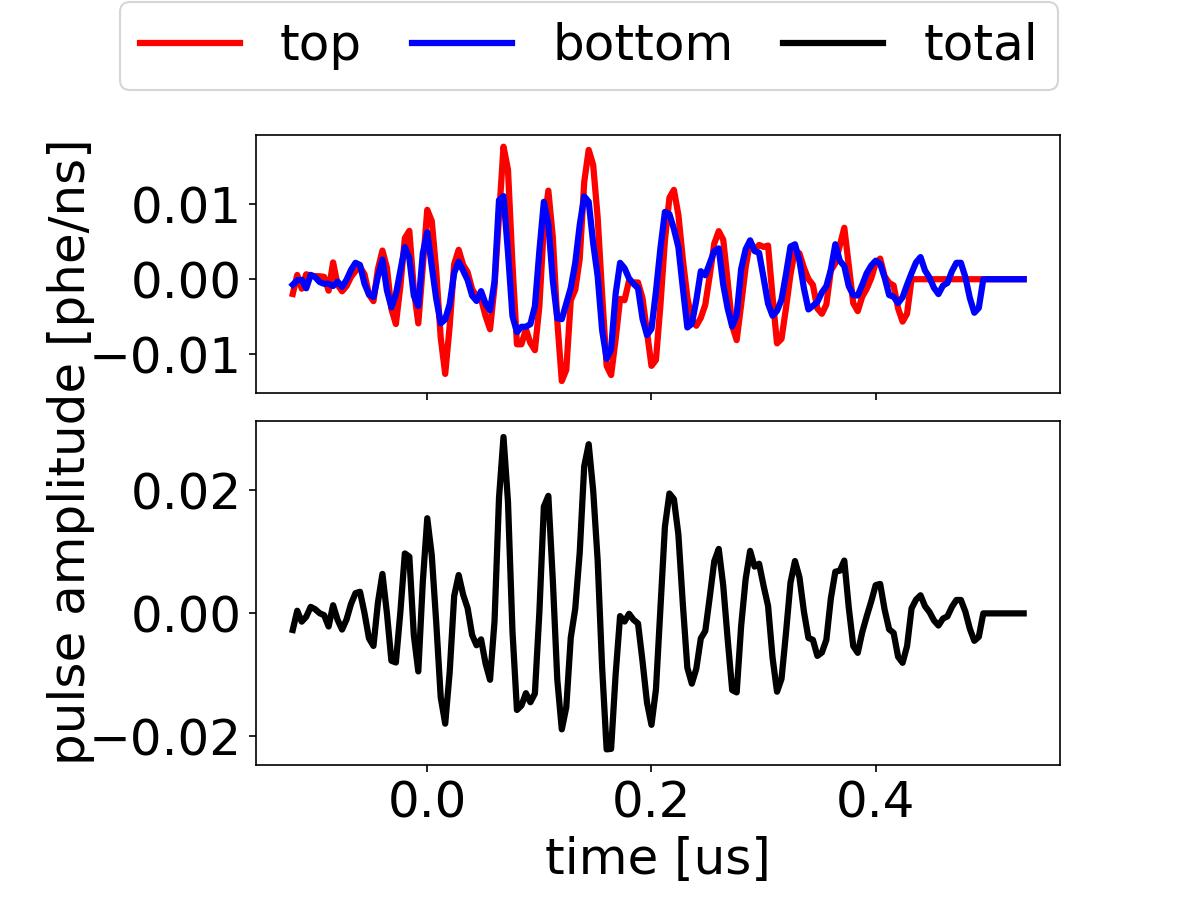
\includegraphics[width=\figurewidth,clip,trim={0 0 0 0}]{Figures/GasTest/exampleWaveforms/proc64767id00000034.jpg}%{Figures/GasTest/CutsValid/wave/testproc65831coinid0.jpg}
	\caption{}
	\label{fig:}
\end{subfigure}
\caption[\gtest\ signal: electronic noise.]{\gtest\ signal: electronic noise signal. (a) An example waveform. Data were taken at \ddtt{2017}{12}{08}{14}{02}, with \opvtvb\ at \SIlist{+6;-6}{kV}, \opgd\ at \standarddensity .%Data were taken at \ddtt{2018}{03}{12}{11}{41} , with \opvtvb\ at \SI{0}{\kV}, \opgd\ at vacuum.
	% proc13001, procid:101001, Aude rename the dataset name, really confusing now.	
}
\label{fig:noise}
\end{figure}

\paragraph{PMT dark current}
\label{sec:events dark current}
PMT dark current usually refers to the signal from the thermal electron emission from the photocathode and dynode surfaces, which are charges generated in the PMT when no photon ejects photoelectrons from the photocathode surface. The thermal electrons from the photocathode surface, like photoelectrons, if landing on the effective area of the first dynode, will be amplified by the PMT and produce a \sphe -like signal. Such \sphe -like signals of the PMT dark current are a major concern, since they are not distinguishable from \sphe s in signals of interest. The thermal electrons from other surfaces may also be amplified by the PMT dynode chain and produce signals that are distinguishably smaller than \sphe , thus drawing less concern. 

A random coinciding of \sphe -like signals (dark current is one of the most common sources of \sphe -like signals) between two PMTs, is called an accidental coinciding signal. The PMTs that are used in this study have a \SI{\sim 1}{\kHz} dark current rate.  This rate leads to a \SI{\sim 3.4}{\Hz} rate of the accidental coinciding signals with regard to CWW of \SI{1.7}{\us}. 
 
 %The \sphe\ source is not limited to dark current. 
\begin{figure}[!p]
	\centering
	\begin{subfigure}[b]{0.7\textwidth}
		\centering
		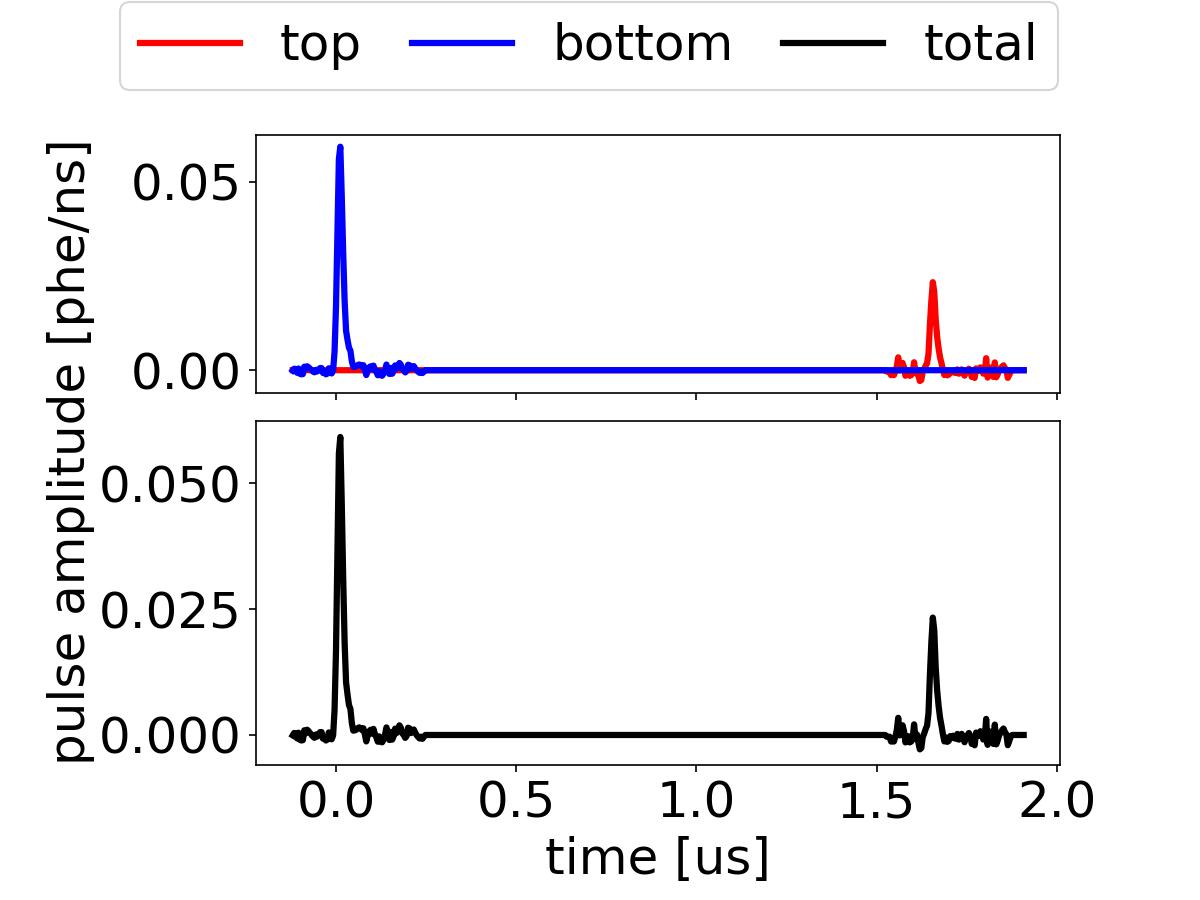
\includegraphics[width=\figurewidth,clip,trim={0 0 0 0}]{Figures/GasTest/exampleWaveforms/proc64767id00000053.jpg}%{Figures/GasTest/CutsValid/wave/testproc65831coinid0.jpg}
		\caption{}
		\label{fig:}
	\end{subfigure}
	\caption[\gtest\ signal: PMT dark current accidental coinciding.]{\gtest\ signal: PMT dark current accidental coinciding. (a) An example waveform. Data were taken at \ddtt{2017}{12}{08}{14}{02}, with \opvtvb\ at \SIlist{+6;-6}{kV}, \opgd\ at \standarddensity .%Data were taken at \ddtt{2018}{03}{12}{11}{41} , with \opvtvb\ at \SI{0}{\kV}, \opgd\ at vacuum.
		% proc13001, procid:101001, Aude rename the dataset name, really confusing now.	
	}
	\label{fig:pmt dark current}
\end{figure}

\todo{should I talk about PMT afterpulsing?}

\paragraph{PTFE fluorescence}
\label{sec:events PTFE fluo}
PTFE fluorescence is the phenomenon in which PTFE emits photons that it absorbed. This delay emission normally appears in forms of \sphe s following a high quantity of photon production, and increase the \sphe\ rate succeeding. The rate of after emission photons (fluorescence rate) roughly follows an exponential decay model:
\begin{align}
	 \text{fluorescence rate} = f_{\text{FR}}\ A\frac{1}{\tau} \exp \left( -\frac{t}{\tau} \right) 
\end{align} 
where $\tau$ is the decay time constant; t is the time since the previous photon production; A is quantity of photons in the previous photon production that are absorb by the PTFE; and $f_{\text{FR}}$ is the fluorescence ratio, which is the ratio of the number of photons emitted after by the PTFE material to the number of photons absorbed by the PTFE material.

Measurements show that fluorescence rates, decay times $\tau$, and fluorescence ratio $f_{\text{FR}}$ have a various range. This might be caused by different conditions of synthesis, as described in Ref.~\cite{Gachkovskii1969}. This effect is also believed to cause the slow decay of electron signal in liquid xenon TPCs. A decay time of \SI{2.3}{\ms} is reported in Ref.\cite{Sorensen2018}. A decay time of \SI{10}{\ms} is reported in internal review in \luxe .  

To illustrate the large rate of \sphe s that follows a large-area signal, we look at 1-\si{\ms} windows before and after a large photon production. In the succeeding 1-\si{\ms} window after t = \num{0}, which is the time when the selected large signal happened, as shown with the selected large signal in Fig.~\ref{fig:ptfe fluo b}, Fig.~\ref{fig:ptfe fluo c}, we see 33 \sphe s. In comparison, we see only 1 \sphe\ in the earlier 1-\si{\ms} window, as shown in the same figure before t = \num{0}. 
%An example waveform of an event with large photon production and the waveform in its preceding and succeeding window is shown in Fig.~\ref{fig:ptfe fluo b}. A waveform in its preceding window is shown in Fig.~\ref{fig:ptfe fluo b} to compare the \sphe\ rate. In the comparison example, 33 \sphe s in a succeeding window of \SI{\sim 1000}{\us} are recorded, when only 1 \sphe\ are recorded in a preceding window with the same window width. 
This increasing rate of \sphe\ increases the probability of accidental coinciding between two PMT channels, as shown in Fig.~\ref{fig:ptfe fluo d}; given the practical choice of our CCW, this random accidental coinciding, like PMT dark current, is a potential source of background that looks like \ees s.
   \begin{comment}
\begin{subfigure}[b]{0.8\textwidth}
\centering
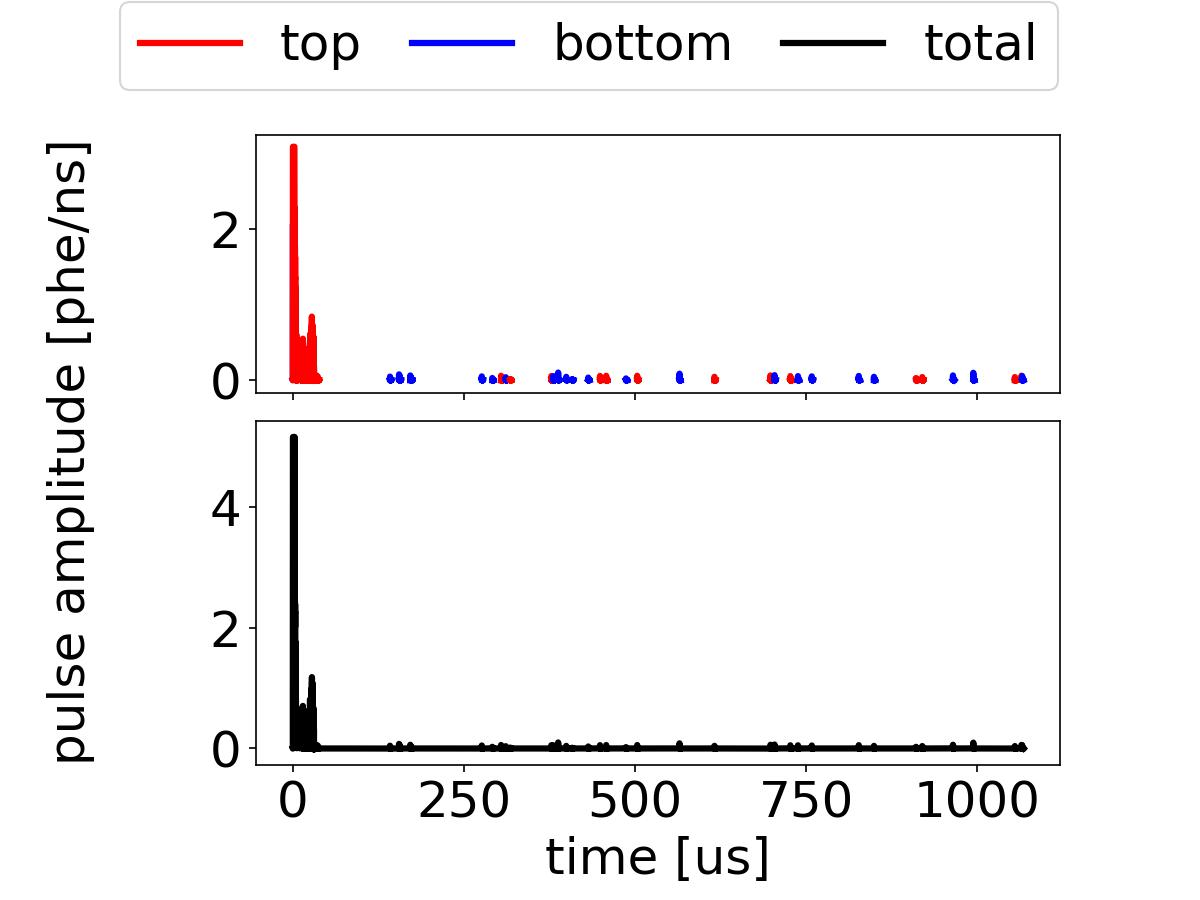
\includegraphics[width=\figurewidth,clip,trim={0 0 0 0}]{Figures/GasTest/exampleWaveforms/proc64767PTFEFluo1.jpg}
\caption{}
\label{fig:ptfe fluo a}
\end{subfigure}
\par\bigskip
\end{comment}
\begin{figure}[!p]
	\centering
   	\begin{subfigure}[b]{1.0\textwidth}
   	\centering
   	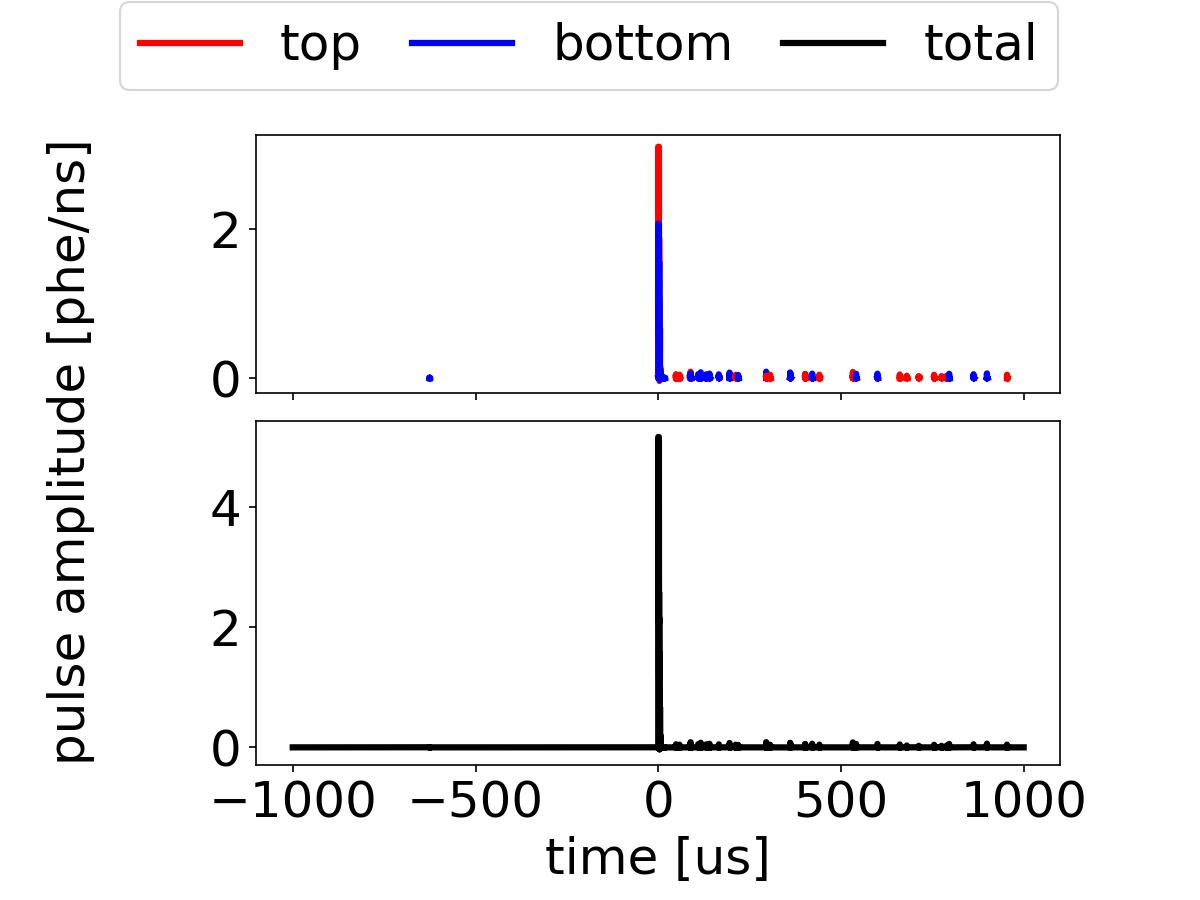
\includegraphics[width=\figurewidth,clip,trim={0 0 0 0}]{Figures/GasTest/exampleWaveforms/proc64767PTFEFluo2x.jpg}
   	\caption{}
   	\label{fig:ptfe fluo b}
   \end{subfigure}
	\caption[\gtest\ signal: PTFE fluorescence after an event with large photon production.]{\gtest\ signal: PTFE fluorescence after an event with large photon production. (a) An example waveform \SI{1000}{\us} before and after a large-area signal. There are more \sphe s after an event with large photon production than before. The \sphe\ rate before this large-area event is representative of the average \sphe\ rate. Data were taken at \ddtt{2017}{12}{08}{14}{02}, with \opvtvb\ at \SIlist{+6;-6}{kV}, \opgd\ at \standarddensity .}
	\label{fig:ptfe fluo}
\end{figure}
\begin{figure}\ContinuedFloat
	\centering
	\begin{subfigure}[b]{0.7\textwidth}
		\centering
		\includegraphics[width=\figurewidth,clip,trim={0 0 0 0}]{Figures/GasTest/exampleWaveforms/proc64767PTFEFluo2P1.jpg}
		\caption{}
		\label{fig:ptfe fluo c}
	\end{subfigure}
	\par\bigskip
	\begin{subfigure}[b]{0.7\textwidth}
		\centering
		\includegraphics[width=\figurewidth,clip,trim={0 0 0 0}]{Figures/GasTest/exampleWaveforms/proc64767PTFEFluo2P2.jpg}
		\caption{}
		\label{fig:ptfe fluo d}
	\end{subfigure}
	\caption[\gtest\ signal: PTFE fluorescence after an event with large photon production (cont.).]{\gtest\ signal: PTFE fluorescence after an event with large photon production (cont.). (b) An example waveform, zoomed in the range of \SIrange{0}{17}{\us}, which shows the signal with large photon production.  (c) An example waveform, zoomed in the range of \SIrange{87}{89}{\us}, which shows PTFE fluorescence induced \sphe s accidental coinciding between the two PMTs. This accidental coinciding signal looks like an \ees .}
	\label{fig:ptfe fluo cont}
\end{figure}

With these examples in mind, we can quantify the fluorescence process by looking at the delayed \sphe\ rate follow large-area signals over different characteristic timescales. The \sphe\ rate of this PTFE fluorescence increase if the ELD has a recent large photon production. Fig.~\ref{fig:PMT PFTE fluo} shows the photon rate after source signals: This photon fluorescence rate increases as the signal area of source signals increases; and this photon fluorescence rate decreases over time. 

\begin{figure}[!p]
	\centering
	\begin{subfigure}[t]{\twofigurewidth}
		\centering
		\includegraphics[width=\textwidth,clip,trim={0 0 0 0},angle=0,origin=c]{Figures/GasTest/DatasetQuality/topPMTPTFEFluoEva64767.jpg}
		\caption{}
		\label{fig:PMT PFTE fluo top}
	\end{subfigure}
	\begin{subfigure}[t]{\twofigurewidth}
		\centering
		\includegraphics[width=\textwidth,clip,trim={0 0 0 0}]{Figures/GasTest/DatasetQuality/botPMTPTFEFluoEva64767.jpg}
		\caption{}
		\label{fig:PMT PFTE fluo bottom}
	\end{subfigure}
	\caption[Photon fluorescence rate after photon production in the ELD.]{Photon fluorescence rate after photon production in the ELD: (a) top PMT; (b) bottom PMT. The solid lines show the medians. The color bands show the \SIrange{25}{75}{\percent} bands. The choice of bin edges is made to get enough statistics in each bin. }
	\label{fig:PMT PFTE fluo}
\end{figure}

An estimation of fluorescence rate, decay time $\tau$, and fluorescence ratio $f_{\text{FR}}$ is carried out by studying the photon rate in the waveform after a signal production of larger than \SI{e4}{\phe} in the range of \SIrange{200}{600}{\us} after the end time of signal. The choice of the smaller value of the succeeding window is to avoid the influence from the anode cone events correlating signals, whereas the choice of the later time of the succeeding window is to avoid the influence the background rate, which is mostly contributed by dark current. In the chosen signal ranges, the background rate is \SI{\sim 1}{\kHz} per PMT, mostly contributed by PMT dark current. This rate is small compared to fluorescence rate (median \SI{\sim 20}{\kHz}) per PMT, thus negligible in this estimation. Therefore,
\begin{align}
	\text{photon rate} & \approx \text{fluorescence rate}\ \big( + \text{background rate (dark current, etc.) \big)} \\
	&\propto \frac{1}{\tau} \exp \left( -\frac{t}{\tau} \right) \label{eqn:fluo}
\end{align} 
To better estimate the photon rate profile and find the decay time $\tau$, we fit this exponential decay profile to binned data in the succeeding window. To combine multiple events to reduce the statistical error, individual events are normalized by their signal areas in the range of \SIrange{0}{1000}{\us} and then co-added by bin; the resulting graph is fitted, and shown in 
%each waveform in the succeeding window is normalized so that the integrated area in the choice of time range is 1. Then, by averaging these normalize waveforms and fitting the average waveform with Eqn.~\ref{eqn:fluo} profile, we get a $\tau$ of \SI{375 \pm 36}{\us}, as shown in 
Fig.\ref{fig:PMT PTFE fluo tau}: $\tau$ of \SI{407 \pm 35}{\us}.

The fluorescence ratio $f_{\text{FR}}$ is defined as,
\begin{align}
f_{\text{FR}} &= \frac{\text{\#\ photons reemitted}}{\text{\#\ photons absorbed}}
\end{align}
which is the ratio of the number of photons that are reemitted from the PTFE after a large-area event to the number of photons that are absorbed by the PTFE in a large-area event. 

The number of photons reemitted is estimated from the exponential decay profile defined above and the number of photons in the succeeding \SIrange{200}{600}{\ns} window after the end of the large-area signal. From the estimated decay time, the ratio of the number of reemitted photons in the succeeding window ($N_{\text{SW}}$) to the total number of reemitted photons is derived, noted as $P_{\text{SW}}$: 

\begin{align}
P_{\text{SW}} \approx& \frac{N_{\text{SW}}}{\text{\#\ photons reemitted}}.
\end{align}

The number of reemitted photons in the succeeding window is estimated from the number of photons reemitted detected in the succeeding window ($A_{\text{SW}}$) and the light collection efficiency for photons starting from PTFE surface:  
\begin{align}
%\text{\#\ photons reemitted} \approx& \frac {
%	\frac{\text{\normalsize \#\ photons in the succeeding window} }
%	{ \text{\normalsize estimated profile ratio of the succeeding window} } 
%	}
%	{\text{\normalsize average light collection efficiency at the location of PTFE}} ,
A_{\text{SW}} \approx& \text{LCE}_{\text{PTFE}} N_{\text{SW}}. 
\end{align}
where $\text{LCE}_{\text{PTFE}}$ is the average light collection efficiency for photons starting from PTFE surface. 
%which is estimated by the same method  described in Section~\ref{sec:gtest light collection}. 

On the other hand, the number of photons absorbed by PTFE is estimated from the total number of photons the source large-area signal ($N_{\text{source}}$) and the light collection simulation of the fraction of photons that PTFE absorbed:
\begin{align}
\text{\#\ photons absorbed} \approx& \text{LCF}_{\text{EL-PTFE}} N_{\text{source}}
\end{align}
where $\text{LCF}_{\text{EL-PTFE}}$ is the average fraction of photons absorbed by PTFE in the simulation with photons starting in the EL region, the location where the source signals happen. 

The total number of photons the source large-area signal ($N_{\text{source}}$) is related to the detected signal area ($A_{\text{source}}$) and light collection efficiency of the source signals in the EL region ($\text{LCE}_{\text{EL}}$).
\begin{align}
%\text{\#\ photons absorbed} \approx& \frac{
%	\frac{\text{\normalsize \#\ photons in the signal}}
%	{\text{\normalsize average light collection efficiency at the location of the EL region}} 
%	}
%	{\text{\normalsize average absorption fraction by PTFE}} .
A_{\text{source}} \approx& \text{LCE}_{\text{EL}}  N_{\text{source}}
\end{align}

Therefore, from the measure ratio of signal area in the succeeding window ($A_{\text{SW}}$) to the source signal area ($A_{\text{source}}$), the result of which is shown in Fig.~\ref{fig:PMT PTFE fluo ratio}, we can derive the fluorescence ratio $f_{\text{FR}}$. 
$P_{\text{SW}}$ is \num{\sim 0.23} with regard to the decay time $\tau$. $\text{LCE}_{\text{PTFE}}$ is \SI{2.85}{\percent} (top PMT: \SI{1.35}{\percent}, bottom PMT: \SI{1.50}{\percent}); $\text{LCE}_{\text{EL}}$ is \SI{1.70}{\percent} (top PMT: \SI{0.85}{\percent}, bottom PMT: \SI{0.85}{\percent}); and $\text{LCF}_{\text{EL-PTFE}}$ is \SI{79.3}{\percent} (top cone: \SI{39.0}{\percent}, bottom cone: \SI{40.3}{\percent}), which are estimated by using the same method as described in Section~\ref{sec:gtest light collection} using PTFE reflectivity of \num{0.4}. With the ratio of $A_{\text{SW}}$ to $A_{\text{source}}$ \num{\sim 0.5e-3}, $f_{\text{FR}}$ is \num{\sim 1.6e-3}. This result has a big uncertainty (up to \num{1e-3}) due to statistic errors, and the systematic errors in the light collection efficiency and the absorption fraction, resulting from the uncertainty in the PTFE reflectivity value. 

\begin{figure}[!p]
		\centering
		\includegraphics[width=.8\textwidth,clip,trim={0 0 0 0},angle=0,origin=c]{Figures/GasTest/DatasetQuality/PMTPTFEFluoTau0200060064767.jpg}
		\caption[The average of scaled waveform in the range of \SIrange{0}{2000}{\us} since source signals.]{The average of scaled waveform in the range of \SIrange{0}{2000}{\us} since source signals. See text for details.}
		\label{fig:PMT PTFE fluo tau}
	\end{figure}

	\begin{figure}[!p]
		\centering
		\includegraphics[width=.8\textwidth,clip,trim={0 0 0 200}]{Figures/GasTest/DatasetQuality/PMTPTFEFluoRatio0200060064767.jpg}
		\caption[The ratio of the number of photon in the range of \SIrange{200}{600}{\us} since source signals to the number of photons in the source signal.]{The ratio of the number of \sphe s in the range of \SIrange{200}{600}{\us} since source signals to the number of \sphe s in the source signal.}
		\label{fig:PMT PTFE fluo ratio}
	\end{figure}


\paragraph{Cherenkov radiation} 
\label{sec:events Cherenkov}
\todo{think about gamma particle induced cherenkov, and whether the calculation is correct.}
Cherenkov radiation is the photon radiation process when a charged particle is traveling through a medium with its speed higher than the speed of light in the medium. The charged particle could be an external charged particle or electrons that originate from energy loss of external particle in the medium. Because of the photon production in Cherenkov radiation process, especially when this process happens in the PTFE materials (and the PMT windows), it is considered to one of the sources of the signals in \gtest . A cartoon for the physical process and an example waveform of extremely narrow pulse are shown in Fig.~\ref{fig:Chrenkov}. %

The quantity of photon production in Cherenkov radiation process is estimated by its theoretical spectrum following Frank–Tamm formula. A simplified approximation for Frank–Tamm formula from Ref.~\cite{Jackson1999} Eqn.~{14.133} shows:
\begin{align}
	\frac{\d I(\omega)}{\d x} = \frac{e^2 \omega}{c^2} \left[ 1-\frac{1}{\beta^2 \epsilon(\omega)} \right] 
	\label{eqn:CherenkovE}
\end{align}
where $\omega$ is the frequency of Cherenkov radiation, I($\omega$) is the energy intensity of frequency $\omega$, $\epsilon$($\omega$) is the relative permittivity of the medium, and $\beta$ is the speed of the charged particle. 
$\omega$ satisfies that $\beta^2 \epsilon$($\omega$) is larger than one, so that the energy intensity is positive.
The number intensity N($\omega$) can be derived from Eqn.~\ref{eqn:CherenkovE}
\begin{align}
	\frac{\d N(\omega)}{\d x} = \frac{\alpha}{c} \left[1-\frac{1}{\beta^2 \epsilon(\omega)} \right] 
	\label{eqn:CherenkovN}
\end{align}
where $\alpha \equiv e^2/\hbar c \approx 1/137$ is the fine structure constant. The total quantities of photons (N) is the integral over frequency and distance of Eqn.~\ref{eqn:CherenkovN}.

%\todo{resolve the 2 pi difference between Jackson and here. 
%	http://large.stanford.edu/courses/2014/ph241/alaeian2/}
% Answer: simple \omega = 2 \pi f

\begin{figure}[!p]
	\centering
	\begin{subfigure}[b]{.4\textwidth}
		\centering
		\includegraphics[width=\figurewidth,clip,trim={0 0 0 0},angle=0,origin=c]{Figures/GasTest/WeiDrawEvent/Cherenkov.jpg}
		\caption{}
		\label{fig:Chrenkov a}
	\end{subfigure}
	\begin{subfigure}[b]{.4\textwidth}
		\centering
		\includegraphics[width=\figurewidth,clip,trim={0 0 0 0},angle=0,origin=c]{Figures/GasTest/WeiDrawEvent/MuonVac.jpg}
		\caption{}
		\label{fig:}
	\end{subfigure}
	\par\bigskip
	\begin{subfigure}[b]{0.6\textwidth}
		\centering
		\includegraphics[width=\figurewidth,clip,trim={0 0 0 0}]{Figures/GasTest/exampleWaveforms/proc64767id00000002.jpg}%{Figures/GasTest/CutsValid/wave/testproc65831coinid0.jpg}
		\caption{}
		\label{fig:Chrenkov b}
	\end{subfigure}
	\caption[\gtest\ signal: Cherenkov radiation in PTFE.]{\gtest\ signal: Cherenkov radiation in PTFE. (a) Cartoon of the process in which Cherenkov radiation is produced in PTFE. The Cherenkov radiation comes from the electrons created in a gamma particle event. (b) Cartoon of the process in which Cherenkov radiation is produced in PTFE after a muon particle crossing the detector. (1) If the detector is in vacuum, even though the muon particle crosses the cone regions, there is no primary scintillation or ionization inside the ELD active volume, and only Cherenkov radiation signals from this muon event in PTFE are observed. (2) A muon particle does not cross the cone regions. Cherenkov radiation signals from this muon in PTFE are observed. (c) An example waveform of a Cherenkov radiation event. Data were taken at \ddtt{2017}{12}{08}{14}{02}, with \opvtvb\ at \SIlist{+6;-6}{kV}, \opgd\ at \standarddensity .%Data were taken at \ddtt{2018}{03}{12}{11}{41} , with \opvtvb\ at \SI{0}{\kV}, \opgd\ at vacuum.
		% proc13001, procid:101001, Aude rename the dataset name, really confusing now.	
	}
	\label{fig:Chrenkov}
\end{figure}

A portion of these Cherenkov radiation photons can be seen by the PMTs, since PTFE is partially transparent to these photons. The duration of Cherenkov radiation event light production is the duration of charged particle energy loss process, which is typically very short (\SIrange{\sim 1}{10}{\ns}). The number of photons ($A_{\text{Che}}$) detected by the PMTs for a typical \SI{1}{\MeV} electron is estimated using the following parameters:  
\begin{align}
	A_{\text{Che}} \approx N_{\text{Che}} f_{\text{to-surface}} \exp \left ( - d_{\text{to-surface}}/d_{\text{atten}} \right ) \text{LCE}_{\text{PTFE}} 
\end{align}
where $N_{\text{Che}}$ is the number of produced Cherenkov radiation photons which the PMTs are sensitive to; $f_{\text{to-surface}}$ is the fraction of Cherenkov radiation photons going toward the PTFE surface; $d_{\text{to-surface}}$ is the distance from the location of Cherenkov radiation produce to the PTFE surface; $d_{\text{atten}}$ is the attenuation length of PMT sensitive Cherenkov radiation photons; and $\text{LCE}_{\text{PTFE}}$ is the light collection efficiency for photons exiting PTFE surfaces. 

$N_{\text{Che}}$ is related to PMT sensitivity, we take the PMT sensitive photon wavelength in the range of \SIrange{160}{650}{\nm} (the spectral response range for PMT R11410-10, as described in Ref.~\cite{HamamatsuPhotonics2006}). $N_{\text{Che}}$ is also related the PTFE refractive index, and electron stopping distance, which are approximately 2 ($\epsilon$ \num{\sim 4}), and \SI{\sim e-1}{\cm} for a \SI{1}{\MeV} electron in PTFE, respectively. The attenuation distance of photons $d_{\text{atten}}$ is \SI{\sim 7}{\cm} for a \SI{1}{\MeV} electron for PTFE, from Ref.~\cite{NIST}. The light collection efficiency $\text{LCE}_{\text{PTFE}}$ is in the range of \SIrange{1.5}{15}{\percent}, as described in Section.~\ref{sec:gtest light collection}. Therefore, taking $d_{\text{to-surface}}$ to be \SIrange{0}{1}{\cm}, and taking $f_{\text{to-surface}}$  to be \SIrange{10}{50}{\percent}, $N_{\text{Che}}$ is \num{\sim 150}, and the estimated number of Cherenkov photons detected by the PMTs is in the range of up to \SI{\sim 10}{\phe}. Even though this estimated number of photons is not very big, however it is large enough to be seen by both PMTs. For a muon, we can do a similar estimation with changing the stopping distance to the full length of muon trajectory in PTFE, which is \SI{\sim 5}{cm}. Therefore, the estimated number of Cherenkov photons detected by the PMTs in a muon event is in the range of up to \SI{\sim 500}{\phe}. The exact number of detected Cherenkov photons is hard to predict precisely because of the complicated geometry of ELD. However, these estimations conclude that Cherenkov events are one of the visible background signals in our detector.
%However, the possibility of seeing these photons still exist. 
%Thus, Cherenkov radiation is still one of the optimal explanations for the extremely narrow pulses.

One of the most convincing evidence is the existence of Cherenkov radiation events is that short-duration signals are seen in the detector at vacuum condition. Fig.~\ref{fig:Chrenkov c} shows the \pud\ vs. signal area plot from a dataset with \opvtvb\ at \SI{0}{\kV}, \opgd\ at vacuum. %The red population seen are the selected extremely narrow pulses. Extremely narrow pulses in vacuum data consist of events that potentially come Cherenkov radiation in PTFE.  
The black box shows the potential events which are considered to be associated with Cherenkov radiation process. Since the detector is at vacuum condition, it is lack of other photon production processes. These potential Cherenkov radiation events may source from both external charged particles and energy loss of external particles, likely an external higher energy photon (gamma radiation), or a cosmic ray muon. This process is described below: An external particle travels through the PTFE cones, lose its energy, ionizes molecules in PTFE and radiates photon along its trajectory. Since muon particles are usually more energetic than other external particles like gamma radiation, the Cherenkov radiation from muon events is usually larger. This is one explanation for the ``hot spot" at (\num{e2},\num{e2}) in Fig.~\ref{fig:Chrenkov c}. When the detector is filled with xenon gas, the muon particle can also ionize xenon gas atoms inside ELD active volume. This process produces scintillation photons and ionization electrons, and the EL process associated with ionization electrons usually increases signal duration. It explains the reason that this ``hot spot" shifts between vacuum data and xenon gas data. Details for explanations of muon events in xenon gas data are in Section.~\ref{sec:muon}. The signals with their area in the range of \SIrange{0}{e2}{\phe} and signal duration in the range of \SIrange{0}{2e2}{\ns} in Fig.~\ref{fig:Chrenkov c} are likely to be Cherenkov radiation events from muons that do not cross the ELD active region and external gamma radiation induced fast electrons in PTFE (and PMT window). The gamma radiation can scatter electrons in PTFE. These fast-moving scattered electrons can also produce Cherenkov radiation light. When the detector is filled with xenon gas, the same physical processes of Cherenkov radiation from muon and gamma radiation remain. Therefore, these processes explain why a similar population of Cherenkov radiation events exist in both vacuum data (Fig.~\ref{fig:Chrenkov c}) and xenon gas data  (Fig.~\ref{fig:Chrenkov d}).

\begin{figure}[!p]
	\centering
	\begin{subfigure}[b]{0.8\textwidth}
		\centering
		\includegraphics[width=\figurewidth,clip,trim={0 0 0 0}]{Figures/GasTest/CutsValid/res65831/pdpa00Vecfig65831rev.jpg}%{Figures/GasTest/CutsValid/all65831.jpg}
		\caption{}
		\label{fig:Chrenkov c}
	\end{subfigure}
	\par\bigskip
	\begin{subfigure}[b]{0.8\textwidth}
		\centering
		\includegraphics[width=\figurewidth,clip,trim={0 0 0 0}]{Figures/GasTest/CutsValid/res64761/pdpa00Vecfig64761rev.jpg}%{Figures/GasTest/CutsValid/all64767.jpg}%{Figures/GasTest/CutsValid/all64731.jpg}
		\caption{}
		\label{fig:Chrenkov d}
	\end{subfigure}
	\caption[\gtest\  \rpd\ vs. signal area.]{\gtest\  \rpd\ vs. signal area. (a) Vacuum data. Data were taken at \ddtt{2018}{03}{12}{11}{41}, with \opvtvb\ at \SI{0}{\kV}, \opgd\ at vacuum. (b) Xenon gas data. Data were taken at \ddtt{2017}{12}{08}{13}{12}, with \opvtvb\ at \SI{0}{\kV}, \opgd\ at \standarddensity . The black solid line indicates the muon events which crosses the cone regions. The black dashed line indicates the muon events which do not cross the cone regions, and might also include gamma radiation events in PTFE. 
		% proc13001, procid:101001, Aude rename the dataset name, really confusing now.	
	}
	\label{fig:ChrenkovCompare}
\end{figure}

\paragraph{Discharge}
\label{sec:microdischarge} 
Discharges happen inside and outside the ELD could produce signals that can be seen by the PMTs.  In sparking tests, we observe discharges on the high voltage feed throughs and cables, which are caused by the smoothness of the high voltage surfaces (especially metallic surfaces) are imperfect. This imperfectness microscopically creates a high field region, and initialized a high ionization probability of the medium (especially gas medium) surrounding it and causes a discharge. The quantity of light production of these discharges has a various range and usually are big. However, depending on the location of the discharge, signals of the discharge have different appearances. The discharges happening outside the ELD may end up having one or several \sphe s in each PMTs with regard to the poor light collection at such location. However, the discharges happening inside the ELD may look like \ees s. 



